\documentclass[oneside,numbers,spanish]{ezthesis}
%\documentclass[oneside,numbers,Spanish]{ezthesis}
%% # Opciones disponibles para el documento #
%%
%% Las opciones con un (*) son las opciones predeterminadas.
%%
%% Modo de compilar:
%%   draft            - borrador con marcas de fecha y sin im'agenes
%%   draftmarks       - borrador con marcas de fecha y con im'agenes
%%   final (*)        - version final de la tesis
%%
%% Tama'no de papel:
%%   letterpaper (*)  - tama'no carta (Am'erica)
%%   a4paper          - tama'no A4    (Europa)
%%
%% Formato de impresi'on:
%%   oneside          - hojas impresas por un solo lado
%%   twoside (*)      - hijas impresas por ambos lados
%%
%% Tama'no de letra:
%%   10pt, 11pt, o 12pt (*)
%%
%% Espaciado entre renglones:
%%   singlespace      - espacio sencillo
%%   onehalfspace (*) - espacio de 1.5
%%   doublespace      - a doble espacio
%%
%% Formato de las referencias bibliogr'aficas:
%%   numbers          - numeradas, p.e. [1]
%%   authoryear (*)   - por autor y a'no, p.e. (Newton, 1997)
%%
%% Opciones adicionales:
%%   spanish         - tesis escrita en espa'nol
%%
%% Desactivar opciones especiales:
%%   nobibtoc   - no incluir la bibiolgraf'ia en el 'Indice general
%%   nofancyhdr - no incluir "fancyhdr" para producir los encabezados
%%   nocolors   - no incluir "xcolor" para producir ligas con colores
%%   nographicx - no incluir "graphicx" para insertar gr'aficos
%%   nonatbib   - no incluir "natbib" para administrar la bibliograf'ia

%% Paquetes adicionales requeridos se pueden agregar tambi'en aqu'i.
%% Por ejemplo:
%\usepackage{subfig}
%\usepackage{multirow}
\usepackage{amsmath}
%\usepackage[spanish]{babel}
%\usepackage[capitalise]{cleveref}
%\usepackage{cleveref}

\newcommand{\addcite}[1][]{\def\tst{#1}\ifx\tst\empty\textcolor{red}{[{\footnotesize REFs}]} \else\textcolor{red}{[{\footnotesize REFs: #1}]} \fi}
\renewcommand{\figurename}{Figura}
\renewcommand{\tablename}{Tabla} 
%% # Datos del documento #
%% Nota que los acentos se deben escribir: \'a, \'e, \'i, etc.
%% La letra n con tilde es: \~n.

\author{N\'estor Ariel  P\'erez Ch\'avez}
\title{Microgeles Polim\'ericos: encapsulado, liberaci\'on de f\'armacos y soluciones coloidales}
\degree{Doctor en Ciencias Qu\'imicas}
\supervisor{Director: Dr. Gabriel S. Longo \\Co-Director: Dr. Alberto G. Albesa}
\institution{Universdad Nacional de La Plata}
\faculty{Facultad de Ciencias Exactas}
\department{Departamento de Qu\'imica}

%% # M'argenes del documento #
%% 
%% Quitar el comentario en la siguiente linea para austar los m'argenes del
%% documento. Leer la documentaci'on de "geometry" para m'as informaci'on.

%\geometry{top=40mm,bottom=33mm,inner=40mm,outer=25mm}

%% El siguiente comando agrega ligas activas en el documento para las
%% referencias cruzadas y citas bibliogr'aficas. Tiene que ser *la 'ultima*
%% instrucci'on antes de \begin{document}.
\hyperlinking
\begin{document}

%% En esta secci'on se describe la estructura del documento de la tesis.
%% Consulta los reglamentos de tu universidad para determinar el orden
%% y la cantidad de secciones que debes de incluir.

%% # Portada de la tesis #
%% Mirar el archivo "titlepage.tex" para los detalles.
%% ## Construye tu propia portada ##
%% 
%% Una portada se conforma por una secuencia de "Blocks" que incluyen
%% piezas individuales de informaci'on. Un "Block" puede incluir, por
%% ejemplo, el t'itulo del documento, una im'agen (logotipo de la universidad),
%% el nombre del autor, nombre del supervisor, u cualquier otra pieza de
%% informaci'on.
%%
%% Cada "Block" aparece centrado horizontalmente en la p'agina y,
%% verticalmente, todos los "Blocks" se distruyen de manera uniforme 
%% a lo largo de p'agina.
%%
%% Nota tambi'en que, dentro de un mismo "Block" se pueden cortar
%% lineas usando el comando \\
%%
%% El tama'no del texto dentro de un "Block" se puede modificar usando uno de
%% los comandos:
%%   \small      \LARGE
%%   \large      \huge
%%   \Large      \Huge
%%
%% Y el tipo de letra se puede modificar usando:
%%   \bfseries - negritas
%%   \itshape  - it'alicas
%%   \scshape  - small caps
%%   \slshape  - slanted
%%   \sffamily - sans serif
%%
%% Para producir plantillas generales, la informaci'on que ha sido inclu'ida
%% en el archivo principal "tesis.tex" se puede accesar aqu'i usando:
%%   \insertauthor
%%   \inserttitle
%%  \insertsupervisor
%%   \insertinstitution
%%   \insertdegree
%%   \insertfaculty
%%   \insertdepartment
%%   \insertsubmitdate

\begin{titlepage}
  \TitleBlock{
\includegraphics[scale = 1.5]{Figures/escudo}}
 % \TitleBlock{\Huge\scshape\insertinstitution}
  \TitleBlock{\Large\scshape\textbf{\insertinstitution}}
  \TitleBlock[\bigskip]{\scshape\textbf{\insertfaculty}}
   \TitleBlock[\bigskip]{\textbf{\insertdepartment}}
%   \TitleBlock{\hline }
   \TitleBlock{\textbf{\underline{\textit{Trabajo de Tesis Doctoral:}}}}
  \TitleBlock{\scshape\inserttitle }
%   \TitleBlock{\hline }

  \TitleBlock{
    \underline{\textbf{\textit{Tesista:}}} \scshape\insertauthor \\
%    para obtener el grado de \insertdegree\\
%dirigado por:\\
\insertsupervisor}
%\TitleBlock{\insertsupervisor}

  \TitleBlock{\underline{\textbf{\textit{A\~no:}}} \insertsubmitdate}
  %\TitleBlock[\bigskip]{\insertdepartment}
\end{titlepage}

%% Nota 1:
%% Se puede agregar un escudo o logotipo en un "Block" como:
%%   \TitleBlock{\includegraphics[height=4cm]{escudo_uni}}
%% y teniendo un archivo "escudo_uni.pdf", "escudo_uni.png" o "escudo_uni.jpg"
%% en alg'un lugar donde LaTeX lo pueda encontrar.

%% Nota 2:
%% Normalmente, el espacio entre "Blocks" se extiende de modo que el
%% contenido se reparte uniformemente sobre toda la p'agina. Este
%% comportamiento se puede modificar para mantener fijo, por ejemplo, el
%% espacio entre un par de "Blocks". Escribiendo:
%%   \TitleBlock{Bloque 1}
%%   \TitleBlock[\bigskip]{Bloque2}
%% se deja un espacio "grande" y de tama~no fijo entre el bloque 1 y 2.
%% Adem'as de \bigskip est'an tambi'en \smallskip y \medskip. Si necesitas
%% aun m'as control puedes usar tambi'en, por ejemplo, \vspace*{2cm}.




%% # Prefacios #
%% Por cada prefacio (p.e. agradecimientos, resumen, etc.) crear
%% un nuevo archivo e incluirlo aqu'i.
%% Para m'as detalles y un ejemplo mirar el archivo "gracias.tex".
%\textbf{Agradecimientos}\\

Al llegar a este punto del camino, no puedo evitar mirar atr\'as y reflexionar sobre el viaje que ha sido completar esta tesis. Ha sido un per\'iodo lleno de desaf\'ios, alegr\'ias, tritezas, mucho aprendizaje, todo un crecimiento personal dir\'ia y claro acad\'emico. Este logro no habr\'ia sido posible sin el apoyo, la gu\'ia y la inspiraci\'on de muchas personas que me acompa\~naron en diferentes etapas de este proceso.

En primer lugar, deseo expresar mi m\'as profundo agradecimiento a mis directores de tesis, Dr. Gabriel S. Longo y Dr. Alberto G. Albesa (Gaby y Beto con cari\~no) cuya experiencia, conocimiento y sobre todo mucha paciencia fueron fundamentales para realizar este doctorado. Gracias por confiar en m\'i en todo este camino.

No quiero mencionar m\'as nombres porque son demasiadas personas a las que tendr\'ia que agradecerle y me parecer\'ia injusto que alguien se quede afuera. Compa\~neres de militancia, de casa, de oficinas, de cer\'amica, f\'utbol, familia, etc, etc. 

No puedo dejar de mencionar a las insituciones que hicieron posible todo esto es decir a CONICET, AGENCIA, al INIFTA, la Facultad de Ciencias Exactas, la Universidad Nacional de La Plata. Y en particular la Laboratorio de Materia Blanda lugar que fue mi segundo hogar y en donde conoc\'i y conviv\'i con personas maravillosas. 

Finalmente, mi gratitud se extiende a todos aquellos que, de una manera u otra, contribuyeron a este trabajo, ya sea a trav\'es de charlas, intercambios acad\'emicos o simplemente ofreciendo su amistad y un mate. A todes ustedes, mi m\'as sincero agradecimiento.

...y a las Umas claro.

\newpage
\thispagestyle{empty}
\null

\chapter{Hoja de ruta}
\label{ruta}

Este cap\'itulo busca guiar al lector en la distribución de la presente tesis. 


En su primer cap\'itulo, nos adentramos en el  mundo de los materiales blandos, la esencia misma de estos materiales y su relevancia en la industria y la ciencia moderna. Se har\'a enfas\'is en los hidrogeles polim\'ericos dentro de los cuales encotraremos a los films y a los micro y nano geles. Las motivaciones y objetivos son presentados. 
 Adem\'as se mencionar\'a el tipo enfoque y las herramientas que se utilizaron para llevar a cabo los estudios presentados en la tesis.

El primer sistema polim\'erico, los films, se retoma en los antecedentes, \ref{Chapter-film}, en la cual se da primera aproximaci\'on de parte de quien les escribe a la Teor\'ia Molecular. Las ventajas del uso de la termodin\'amica estad\'istica y como su combinaci\'on con las propiedades moleculares de los sistemas nos permite explicar toda la termodin'amica necesaria para la descipci\'on y predicci\'on de su comportamiento en condiciones determinadas.  
Se  revisan conceptos generales del comportamiento de estas cadenas polim\'ericas entrecruzadas en soluci\'on.
En part\'icular se mostrar\'a la respuesta  de los films poliméricos a cambios en el pH y la concentraci\'on de sal.  En este capitulo también encontraremos resultados sobre la aplicabilidad en el secuestro de dos prote\'inas modelos (citocromo y mioglobina), la elección de estos resultados, respuesta a pH, concentraci\'on salida, adsoric\'on de prote\'inas,  es debido a que los mismos son retomados en los cap\'itulos subsecuentes.

Es importante destacar que en  el transcurso de este aprendizaje logró la presentación de trabajos en donde se hace uso de los films polim\'ericos en el secuestro de moleculas, con aplicabilidad en la agroqu\'imcia  \addcite[film - glifosato], y principalmente en su uso de secuestro de f\'armacos \addcite[polimainas] trabajo con el cual nos acercamos  a los objetivos del presente trabajo.


Emocionado por su primer éxito, Carlos se aventuró en el siguiente capítulo: los micro y nano geles poliméricos. Descubrió que estos geles eran como pequeñas partículas con habilidades especiales, capaces de responder a estímulos externos y adaptarse a diferentes entornos. A medida que profundizaba en su investigación, Carlos comprendió la importancia de diferenciar entre micro y nano geles, explorando los métodos utilizados para sintetizarlos y caracterizarlos en el laboratorio. Fascinado por las aplicaciones emergentes de estos geles, desde la entrega de medicamentos hasta la ingeniería de tejidos, Carlos comenzó a trazar conexiones entre los films poliméricos y los geles poliméricos, revelando un mundo de posibilidades interconectadas.

Guiado por su deseo de exploración y conocimiento, Carlos pasó al siguiente capítulo: la metodología experimental. Aquí, descubrió los secretos detrás de los experimentos y análisis rigurosos. Se adentró en los materiales utilizados en su investigación y aprendió los procedimientos precisos para sintetizar tanto los films poliméricos como los micro y nano geles poliméricos. Cada paso, cada reacción química, se convirtió en un viaje hacia la comprensión y la perfección.

Después de meses de trabajo duro y dedicación, llegó el momento más esperado: los resultados y la discusión. Carlos presentó sus hallazgos al mundo, revelando datos reveladores y sorprendentes. A medida que profundizaba en la interpretación de los resultados, Carlos se sintió como un mago de la ciencia, conectando los puntos y desvelando nuevos conocimientos. Compartió sus conclusiones con la comunidad científica, analizando la relevancia de su trabajo y las posibles áreas de mejora.

Finalmente, Carlos escribió las conclusiones de su tesis. En este capítulo final, resumió sus descubrimientos y evaluó el éxito de sus objetivos. Reconociendo el valor de su investigación, Carlos compartió las contribuciones que su trabajo podría hacer al campo de estudio. Con entusiasmo, dejó abierta la puerta para futuras investigaciones, instando a otros a continuar su legado y desafiar los límites del conocimiento científico.

Y así, el viaje de Carlos llegó a su fin. Con su tesis completada, se despidió del mundo de los films poliméricos y los micro y nano geles poliméricos, pero no sin llevar consigo un tesoro invaluable: el conocimiento y la pasión por la ciencia. Su historia se convirtió en una inspiración para otros, recordándoles que el poder del descubrimiento y la investigación puede llevar a un futuro lleno de innovación y avance científico.

Y así, el cuento de Carlos y su "hoja de ruta" de tesis llega a su fin, pero el comienzo de un nuevo capítulo para aquellos que se atrevan a explorar los misterios y las maravillas de los materiales poliméricos.



En los siguientes capitulos ...
El estudio de estos dispositivos intelgientes a trav\'ez de m\'etodos te\'orico/computacionales no es muy distinto al realizado en un proyecto experimental. El planteo de la composici\'on y estrucutra de nuestros geles, as\'i como tambi\'en el barrido de variables,llamese pH, temperatura, concentraci\'on de sal, es realizado de manera sistem\'atica.
La ventaja de utilizar m\'etodos computacionales es que nos permiten explicar los fenomenos observables a partir del cambio de variables controladas en el laboratorio.
El planteo de teor\'ias que nos ayuden a obtener la informaci\'on termodin\'amica de cada sistema son la base para la presente tesis... 


Al igual que en un proyecto experimental, nuestra idea es poder identifcar las condiciones \'optimas en las cuales los geles puedan ser usados como biomateriales inteligentes. 
La identificaci\'on de estas condiciones es llevado a cabo utilizando teor\'ias que emplean la termodi\'amica estad\'istica. En part\'icular este trabajo hace uso de la Teor\'ia Cl\'asica de la Densidad. Esta \'ultima tendr\'a algunas variaciones dependiendo el tipo de modelado que se use, el cual ser\'a espicificado y explicado en cada uno de los sistemas presentados.

En part\'icular en este cap\'itulo se dar\'a un vistazo general de la Teor\'ia Molecular derivada de la teor\'ia cl\'asica de la densidad. 
Al final del mismo tambi\'en se introducir\'a sobre el tipo de modelado utulizado para poder implementar las teor\'ias....
 


%% # 'Indices y listas de contenido #
%% Quitar los comentarios en las lineas siguientes para obtener listas de
%% figuras y cuadros/tablas.
\tableofcontents
\listoffigures
\listoftables

%% # Cap'itulos #
%% Por cada cap'itulo hay que crear un nuevo archivo e incluirlo aqu'i.
%% Mirar el archivo "intro.tex" para un ejemplo y recomendaciones para
%% escribir.
%% Los cap'itulos inician con \chapter{T'itulo}, estos aparecen numerados y
%% se incluyen en el 'indice general.
%%
%% Recuerda que aqu'i ya puedes escribir acentos como: 'a, 'e, 'i, etc.
%% La letra n con tilde es: 'n.

\chapter{Introducci\'on}
\label{Chapter1} % Change X to a consecutive number; for referencing this chapter elsewhere, use \ref{ChapterX}

%----------------------------------------------------------------------------------------
%	SECTION 1
%----------------------------------------------------------------------------------------

\section{Hidrogeles polim\'ericos}

%%%%%%%%%%%%%%%
%%%%%%%%%%%%%%%recorte

\begin{color}{blue}
Durante la decada pasada el uso de materiales blandos ha sido de mucho interes debido a la cantidad de materiales e innovaciones que se optienen con ellos.
La versatilidad de estos los han convertido en materiales  importantes en una amplia variedad de aplicaciones tecnológicas.
Se han utilizado como  espumas y adhesivos, son excelente detergentes, est\'an presentes en la industria de los  cosméticos y pinturas, adem\'as de ser ampliamente usados en aditivos alimentarios . El campo de la medicina, la industria farmaceutica, ha encontrado en estos materiales una oportunidad para la creaci\'on de de trasnportadores de drogas m\'as eficientes biocompatibles y biodegradables.
En estas ultimas aplicaciones los  films y geles  polim\'ericos han sido pioneros en su uso y han tenido un creciente inter\'es.
La capacidad de adsorber solventes y la estructura de cadenas entrelazadas proporciona condiciones adecuadas para la adsorcion y protecci\'on de adsorbatos de inter\'es. \addcite 
\end{color}

En particular los hidrogeles consisten en una red de pol\'imeros reticulares (entrecruzados) altamente hidratados y generalmente biocompatibles. Estos materiales pueden parecerse a los tejidos biol\'ogicos y pueden ser dise\~nados para responder a cambios ambientales como variaciones en la temperatura, el pH, la fuerza i\'onica y la concentraci\'on de algunas biomol\'eculas. Como resultado, los hidrogeles polim\'ericos son actualmente candidatos prometedores para el desarrollo de una variedad de biomateriales con aplicaciones en biosensores, ingenier\'ia de tejidos, regeneraci\'on \'osea, materiales biomim\'eticos, administraci\'on de medicamentos y muchas otras aplicaciones biom\'edicas. \cite{Daly2020}
	
	
Inmersas en soluciones acuosas, estos hidrogeles pueden incorporar y retener grandes cantidades de agua, y de manera m\'as general el solvente en el cual se encuentren inmersos, dentro de su estructura polim\'erica.
Sin embargo, la caracter\'istica m\'as llamativa de estas sistemas es su capacidad para adsorber o liberar estos solventes y cambiar de tama\~no en respuesta a una variedad de est\'imulos externos.
El entorno acuoso dentro de los hidrogeles puede proteger a las prote\'inas de la desnaturalizaci\'on y agregaci\'on, mientras que estas se mantienen activas y estructuradas cuando se liberan de los hidrogeles. \addcite
En la administraci\'on oral de medicamentos, los hidrogeles con respuesta al pH han sido ampliamente investigados como veh\'iculos funcionales que pueden encapsular y liberar prote\'inas, evitando su degradaci\'on en el entorno gastrointestinal. \addcite
Este comportamiento de respuesta es  generalmente reversible y depende de la composici\'on qu\'imica de la red polim\'erica.


\section{Respuesta a estimulo pH, sal y Temperatura}

	
Los microgeles compuestos por cadenas polim\'ericas que tienen segmentos \'acidos como el \'acido acr\'ilico o metacr\'ilico (AA y MAA, respectivamente) se hinchan-deshinchan muchas veces en respuesta a cambios en el pH de la soluci\'on que los contienen \cite{snowden1996colloidal}.
El pH en el cual se marca el inicio y caracteriza esta transici\'on es el pKa aparente del microgel, que depende de la concentraci\'on de sal de la soluci\'on y frecuentemente difiere del pKa intrí\'iseco del mon\'omero \'acido.
Estos microgeles tambi\'en ajustan su tama\~no en respuesta a cambios en la concentraci\'on de sal de la soluci\'on \cite{snowden1996colloidal}.
	
An\'alogamente, los microgeles de algunos pol\'imeros termosensibles experimentan una transici\'on de fase de volumen (VPT por sus siglas en ingl\'es) cuando se calientan por encima de una temperatura caracter\'istica (VPTT o $T_{pt}$) \cite{Pelton1986,Pelton2000}.
Este comportamiento se origina porque tales pol\'imeros son insolubles en agua por encima de cierta temperatura de soluci\'on cr\'itica m\'as baja (LCST) \cite{Kawaguchi2020}.
Normalmente, la LCST del pol\'imero y la VPTT de la red  son aproximadamente id\'enticas. 
Este es el caso de las part\'iculas de microgel de poli(N-isopropilacrilamida) (PNIPAm) \cite{Pelton1986}, cuyo volumen colapsa por encima de $32   ^\circ C$, siendo le mismo para el  pol\'imero lineal \cite{Schild1992}.
	
Al tener un VPTT alrededor de la temperatura corporal, los microgeles de PNIPAm han generado un gran inter\'es para aplicaciones biom\'edicas \cite{Guan2011}.
Las estrategias para controlar el VPTT de los microgeles incluyen la s\'intesis de nuevos mon\'omeros termosensibles  \cite{Cai2007,Macchione2019}, as\'i como la copolimerizaci\'on con un mon\'omero i\'onico o ionizable  \cite{Hirose1987,Lopez2020}.
Este \'ultimo enfoque produce microgeles de respuesta m\'ultiple que son susceptibles a cambios en la temperatura, el pH y la concentraci\'on de sal  \cite{snowden1996colloidal, Farooqi2017}.
Los microgeles de NIPAm y AA han sido ampliamente estudiados \cite{Morris1997, Jones2000,Bradley2005,Begum2016};
Tambi\'en se han investigado microgeles de copol\'imeros de NIPAm y MAA  \cite{Dowding2000,Hoare2004,Giussi2015}.
El VPTT de estos microgeles de respuesta m\'ultiple depende del pH de la soluci\'on y la concentraci\'on de sal, y la fracci\'on de mon\'omero ionizable en las cadenas de pol\'imero  \cite{Morris1997,Jones2000, Hoare2004, Bradley2005, Lee2008,Wong2009,Hamzavi2016}.



\section{Encapsulado y Liberaci\'on de medicamentos}

El inter\'es en hidrogeles en especial aquellos con di\'ametros menores a 200 nm ha crecido rotudamente debido a su tiempo m\'as prolongado de circulaci\'on en el sistema circulatorio. La naturaleza incipientemente hidrof\'ilica de estas estructuras, los nanogeles son generalmente biocompatibles y poseen una gran capacidad para incorporar mol\'eculas hu\'esped o analitos, tanto org\'anicos como inorg\'anicos, y prevenir su degradaci\'on por el medio externo. El ambiente acuoso dentro de los hidrogeles puede proteger a las prote\'inas de la desnaturalización y la agregaci\'on [11y13], mientras permanecen activas y estructuradas cuando se liberan de los hidrogeles [14]. En la administraci\'on oral de f\'armacos, los hidrogeles con respuesta de pH se han investigado en gran medida como veh\'iculos funcionales que pueden encapsular y administrar prote\'inas, evitando su degradaci\'on en el entorno gastrointestinal [15-17].
Adem\'as, su escaso tama\~no les permite responder r\'apidamente luego de recibir el est\'imulo \cite{tanaka1979kinetics} . Por todas estas razones, los nanogeles polim\'ericos son hoy en d\'ia una de las primeras opciones consideradas al dise\~nar biomateriales con funciones espec\'ificas \cite{soni2016nanogels, sabir2019polymeric}. El est\'imulo que dispara la respuesta de los nanogeles puede ser suministrado por un gradiente en la composici\'on fisiol\'ogica, ya sea natural o inducido por un estado patol\'ogico. La versatilidad de estos materiales dif\'icilmente puede ser alcanzada con otro tipo de nanopart\'iculas, incapaces de responder a cambios en las condiciones del medio que pueden ser relativamente moderados. El desaf\'io en la actualidad es aprender a controlar esta respuesta para canalizarla en diferentes aplicaciones.


Por citar, \citet{Brugger2008} encontraron que el pH durante la s\'intesis tiene un impacto significativo en la composici\'on y, por lo tanto, en las propiedades del microgel y su capacidad para ser utilizado como un estabilizador sensible a est\'imulos.
Resultados similares fueron estudiados por otros autores en donde se destaca el uso de emulsiones sensibles al pH, la sal y la temperatura  \cite{Ngai2005,Ngai2006, Schmidt2011} o como plantillas para el ensamblaje de nanomateriales \cite{Wong2009}.
Haciendo de estos sistema no solo valiosos en el encapsulado y liberaci\'on de medicamentos, sino también como secuestradores de diferentes adsorbatos.

Del mismo modo \citet{Culver2017A}han utilizado nanogeles de poli(NIPAm-co-MAA) funcionalizados para la uni\'on y detecci\'on de diferentes prote\'inas. 
Recientemente se investigaron dispositivos basados en microgeles de poli(NIPAm-co-MAA) para la encapsulación/liberaci\'on del f\'armaco quimioterap\'eutico Doxorrubicina \cite{Giussi2020, MartinezMoro2020, Pergushov2020}. Estos autores mostraron que el uso de microgeles para la liberaci\'on contralada de sustancias bioactivas con carga opuesta. 
La incorporaci\'on del comon\'omero \'acido proporciona un mecanismo controlado por el pH para la captaci\'on/liberaci\'on de mol\'eculas con carga opuesta, lo que hace que los microgeles de respuesta m\'ultiple sean atractivos para el dise\~no de sistemas funcionales de administraci\'on de f\'armacos \cite{Liu2017}.

En sitentesis el  rango de las potenciales aplicaciones biom\'edicas de los nanogeles es extenso e incluye desarrollos,mas especificamente en medicina, contra los trastornos neurol\'ogicos, las enfermedades cardiovasculares, oftalmol\'ogicas, inflamatorias y autoinmunes, as\'i como tambi\'en avances en el diagn\'ostico por im\'agenes, la ingenier\'ia de tejidos, la reconstrucci\'on \'osea y el manejo de la diabetes y el dolor. Por ejemplo, los nanogeles de \'acido hialur\'onico est\'an siendo evaluados para inhibir la acumulaci\'on de la prote\'ina beta-amiloide en el manejo del Alzheimer. En el tratamiento de la diabetes, se investigan nanogeles sensibles a la glucosa y nuevos m\'etodos de administraci\'on de insulina basados en nanogeles.

Los nanogeles de pol\'imeros termosensibles pueden ser utilizados para la administraci\'on localizada de anest\'esicos. Como veh\'iculos para el suministro de drogas, los nanogeles polim\'ericos pueden administrar f\'armacos de peso molecular bajo, oligonucle\'otidos, prote\'inas terap\'euticas e incluso combinaciones de drogas, lo cual es esencial en terapias contra el c\'ancer y las enfermedades infecciosas.

En muchos casos, la v\'ia oral es preferible para la administraci\'on de f\'armacos, ya que es menos invasiva y presenta otras ventajas que mejoran la calidad de vida de los pacientes. En este \'ambito, los nanogeles con respuesta al pH son de particular inter\'es debido a los cambios de pH que ocurren a lo largo del tracto digestivo, desde un medio \'acido en el est\'omago (pH 1.2-2) hasta uno neutro o moderadamente alcalino en el intestino delgado (pH 7-8). Adem\'s, algunos compartimentos celulares involucrados en la captaci\'on de f\'armacos, como los endosomas tempranos, tienen un pH levemente \'acido. La diferencia de pH que existe entre la superficie de la piel  y el torrente sangu\'ineo puede ser aprovechada para la administraci\'on transd\'ermica de f\'armacos utilizando nanogeles con respuesta al pH [48]. Por otro lado, el microambiente alrededor del tejido canceroso puede presentar un pH m\'as ácido en comparaci\'on con las condiciones fisiol\'ogicas habituales [49-52], por lo que los nanogeles con respuesta al pH est\'an siendo evaluados para la administraci\'on de medicamentos en el tratamiento del c\'ancer [33,53]. Por ejemplo, se han utilizado nanogeles de quitina para la administraci\'on de doxorubicina en diferentes tipos de c\'ancer, incluyendo pulm\'on, mama, h\'igado y pr\'ostata [54]. Del mismo modo, los nanogeles de pol\'imeros termosensibles tienen un gran potencial para la liberaci\'on dirigida tanto a c\'elulas cancerosas como a tejidos inflamados o lesionados, los cuales presentan una temperatura ligeramente superior a la corporal.

	


	
\begin{color}{red}
En este contexto, nuestro esta tesis tiene como objetivo avanzar en el entendimiento b\'asico de la fisicoqu\'imica que subyace en la actuaci\'on de los geles polim\'ericos como biomateriales y su interacci\'on con prote\'inas y otras biomol\'eculas. Adem\'as, esta investigaci\'on busca explorar nuevas estrategias de funcionalizaci\'on de estos hidrogeles para controlar su respuesta e interacci\'on. Para lograrlo, utilizaremos simulaciones moleculares por computadora, las cuales nos brindan acceso a informaci\'on esencial que a menudo no est\'a disponible en el laboratorio. Al mismo tiempo, el conocimiento adquirido en nuestros estudios tiene como objetivo guiar el dise\~no en el laboratorio de geles polim\'ericos con propiedades \'optimas para aplicaciones espec\'ificas en el campo de los biomateriales.

\end{color}

\section{Enfoque te\'orico}


El control de la funci\'on y el comportamiento de un biomaterial requiere comprender su interacci\'on con las prote\'inas. Por ejemplo, las lentes de contacto basadas en \'acido poli(metacr\'ilico) (PMAA) con respuesta al pH est\'an expuestas al fluido lagrimal, que contiene cientos de prote\'inas. La adsorci\'on de algunas de estas prote\'inas debe evitarse, ya que afecta la comodidad de uso y puede provocar inflamaci\'on; sin embargo, la adsorci\'on selectiva de prote\'inas con propiedades antibacterianas y antiinflamatorias, como la lisozima, podr\'ia ser beneficiosa. 
La interacci\'on entre prote\'inas y superficies polim\'ericas est\'a gobernada por una compleja interacci\'on entre diferentes grados de libertad. La capacidad tanto del adsorbato como del material adsorbente para protonar/deprotonar, regular su carga el\'ectrica y modificar el entorno cercano, contribuye a esta complejidad.

\textcolor{red}{Descripcion de diferentes teorias para explicar comportamiento de estos nanogles, diferentes escalas de modelado. Resultados obtenidos...}.

El comportamiento de los microgeles de poli(NIPAm-co-MAA), incluido su VPT y la interacci\'on con pol\'imeros de carga opuesta, se ha descrito aplicando teor\'ias  y simulaciones moleculares en varios niveles de resoluci\'on para investigar el comportamiento de los microgeles polim\'ericos sensibles a est\'imulos \cite{ahualli2016coarse,Landsgesell2019SM}.
\citet{quesada2011gel} ha simulado el comportamiento de geles compuestos  polielectrolitos y termosensibles utilizando  simulaciones de Monte Carlo, logrando explicar el comportamiento de hinchamiento de estas part\'iculas.
\citet{ahualli2016coarse}
enplearon simulaciones de grano grueso empleadas para geles polielectrol\'iticos. Este enfoque computacional,se basaron en interacciones part\'icula-partícula entre unidades de pol\'imero. 

En estos trabajos se han centrado principalmente en el hinchamiento y otras propiedades de las part\'iculas que tienen una red de pol\'imero permanentemente cargada , y algunos han abordado el efecto de la temperatura y la calidad del solvente \cite{Jha2011, QuesadaPerez2013, moncho-jorda2016a, ahualli2016coarse, AdroherBenitez2017PCCP}.
Recientemente, estudios  con simulaciones han considerado la respuesta al pH de microgeles compuestos de pol\'imeros reguladores de carga \cite{Schroeder2015,Rud2017,Sean2018, Hofzumahaus2018,Lu2019}.
Sin embargo, solo unos pocos trabajos te\'oricos han investigado las propiedades de los microgeles de respuesta m\'ultiple en funci\'on de la temperatura, el pH y la concentración de sal  \cite{CaprilesGonzalez2008,polotsky2013collapse}.

\citet{polotsky2013collapse} basa su teor\'ia en equilibrios osm\'oticos y teniendo en cuenta expl\'icitamente el equilibrio de ionizaci\'on dentro de sus microgeles. Llegando a predecir patrones complejos en la dependencia de las dimensiones de las part\'iculas de microgel. Es decir sus par\'ametros de control.
	

\section{Antecedentes}

Para estudiar todos los sistemas que presentaremos en cada cap\'itulo, aplicaremos una teor\'ia molecular.
Este enfoque te\'orico permite describir el tama\~no, la forma, la distribuci\'on de carga, el estado de protonaci\'on y la conformaci\'on de todas las especies moleculares que constituyen al sistema. 
Mediante el uso de teor\'ia a nivel molecular, se ha logrado estudiar la termodin\'amica de hidrogeles de cadenas de poli\'acido reticuladas, incluyendo pel\'iculas delgadas depositadas en superficies \cite{longo2012molecular} y pel\'iculas grafteadas en superficies \cite{longo2014non} en estos trabajos se ha investigado el rol que cumple los cambios en el pH y la concetranci\'on de sal respectivamente. En otros trabajos se ha aplicado este marco te\'orico para considerar la adsorci\'on de p\'eptidos y prote\'inas en nanofilmes de hidrogel de cadenas de poli\'acido entrecruzadas \cite{longo2014equilibrium,narambuena2015lysozyme,longo2016adsorption} observadose el trabajo no trivial que tiene el pH al momento de protonar/deprotonar a los distintos adsorbatos. El m\'etodo que usaremos representa una extensi\'on de las teor\'ias moleculares desarrolladas por Szleifer y colaboradores para investigar la adsorci\'on de prote\'inas en capas de pol\'imeros \cite{hagemann2018use,szleifer1997protein,fang2005kinetics}, y el comportamiento de capas de polielectrolitos d\'ebiles \cite{nap2006weak}. Las predicciones de esta teor\'ia se han demostrado estar en excelente acuerdo cuantitativo con observaciones experimentales para una variedad de sistemas polim\'ericos \cite{tagliazucchi2010responsive,wu2007behavior}.
Estos resultados se lograron mediante la formulaci\'on de una energ\'ia libre general que incluye todas las contribuciones relevantes de estos sistemas polim\'ericos: el equilibrio \'acido-base, la p\'erdida entr\'opica de confinamiento molecular, los grados de libertad conformacionales de la red y las prote\'inas (o adsorbatos en general), y las interacciones electrost\'aticas, de Van der Waals y est\'ericas. En estos trabajos se ha buscado comprender c\'omo la adsorci\'on en estas pel\'iculas de hidrogel depende del pH y la concentraci\'on de sal, tanto en soluciones de prote\'inas individuales como en mezclas. En este m\'etodo, el estado de protonaci\'on de los residuos de prote\'inas y de los segmentos de la red no se asume a priori en funci\'on del pH de la soluci\'on (el seno o bulk), sino que se predice localmente como resultado de la posici\'on del grupo y su entorno local. Nuestros estudios resaltan el papel no trivial que desempe\~na la protonaci\'on de los amino\'acidos en la adsorci\'on de prote\'inas. 

En esta secci\'on nos valdremos de una  red polim\'erica que da estructura a un film polim\'erico. Este sistema nos ayudar\'a a introducirnos en la teor\'ia molecular, as\'i como tambi\'en a eplicar algunos concentos que nos ser\'an de suma importancia en los pr\'oximos cap\'itulos.



\section{Metodolog\'ia}

\subsection{Teor\'ia Molecular}

La teor\'ia es un enfoque de funcional de densidad en el cual los campos de interacción se determinan de manera autoconsistente al considerar modelos muy detallados para cada uno de los componentes moleculares del sistema. Obtenemos informaci\'on estructural detallada, as\'i como propiedades termodin\'amicas. En particular, es posible mostrar el fuerte acoplamiento que existe entre el estado termodin\'amico y la estructura del sistema. De esta manera, se puede estudiar c\'omo las variaciones en las condiciones de la soluci\'on, por ejemplo, la fuerza i\'onica y el pH, entre otros, cambian las propiedades termodinámicas.

La teor\'ia se deriva al escribir la energ\'ia libre del sistema como un funcional de las densidades de las especies en soluci\'on, las conformaciones (en esta tesis de la red polim\'erica) y el potencial electrost\'atico, considerando expl\'icitamente los equilibrios \'acido-base y redox. A continuación, proporcionaremos una derivación detallada de la teoría con especial énfasis en la aplicación novedosa para incluir grupos redox, así como el equilibrio con un electrodo. Para obtener una derivación detallada de la teoría con una discusión extensa de sus ventajas y limitaciones, se remite al lector a las referencias 34-36.



\subsection{Monte Carlo}

El m\'etodo de Metropolis-Monte Carlo \addcite se fundamenta en la generaci\'on aleatoria de n\'umeros y la evaluaci\'on de distintos estados o configuraciones del sistema en estudio. En cada paso de la simulaci\'on, se selecciona de manera aleatoria una configuraci\'on y se calcula su energ\'ia o probabilidad seg\'un un modelo predefinido. Este modelo debe poder describir las interacciones entre los componente del sistema, en nuestro caso son las part\'iculas de nanogeles y el solvente.

\subsection{Dinamica Molecular}


%%%%%%%%%%%%%%%%%recorte
%%%%%%%%%%%%%%%%%%%%


%-----------------------------------
%	SUBSECTION 1
%-----------------------------------
\section{Objetivos}

Los {\bf objetivos específicos} del presente plan de trabajo son los siguientes:
%
\begin{enumerate}
\item Desarrollar un modelo mecano-estadístico utilizando TM para describir la respuesta a cambios de pH, temperatura y concentración de sal en microgeles formados por homopolímeros.%\label{objetivo_1}
\item Extender dicho modelo para investigar el comportamiento de microgeles de copolímeros con respuesta a múltiples estímulos.%\label{objetivo_2}
\item Estudiar los mecanismos de adsorción de diferentes biomoléculas en los microgeles en función de las condiciones del medio y la estructura/composición química de las cadenas poliméricas.%\label{objetivo_3}
\item Desarrollar un modelo combinando simulaciones de TM y Dinámica Molecular (DM) para estudiar el comportamiento de estos microgeles en soluciones relativamente concentradas.%\label{objetivo_4}
\end{enumerate}
%

Finalmente el \textbf{objetivo general} de esta tesis consiste en \emph{desarrollar una descripción comprensiva del comportamiento y respuesta a estímulo de los microgeles poliméricos mediante el uso de modelos teóricos y computacionales basados en las interacciones moleculares.}

% Chapter 2

\chapter{Films polim\'ericos} % Main chapter title

\label{Chapter2} % For referencing the chapter elsewhere, use \ref{Chapter1}

%\section{papers of films}


Los films polim\'ericos o hidrogeles  consisten en una red de pol\'imeros entrecruzados altamente hidratados, generalmente biocompatibles, dependendiendo de su composici\'on qu\'imca. Estos materiales pueden parecerse al tejido biol\'ogico y dise\~narse para responder a cambios ambientales como variaciones de temperatura, pH, fuerza i\'onica y en la concentraci\'on de algunas biomol\'eculas. Como resultado, los hidrogeles polim\'ericos actualmente son candidatos prometedores para el desarrollo de una variedad de biomateriales con aplicaciones para biodetección [1,2], ingenier\'ia de tejidos [3,4], regeneraci\'on \'osea [5], materiales biomim\'eticos [6,7], administraci\'on de f\'armacos [8,9] y muchas otras aplicaciones biom\'edicas [10]. El ambiente acuoso dentro de los hidrogeles puede proteger a las prote\'inas de la desnaturalización y la agregaci\'on [11e13], mientras permanecen activas y estructuradas cuando se liberan de los hidrogeles [14]. En la administraci\'on oral de f\'armacos, los hidrogeles con respuesta de pH se han investigado en gran medida como veh\'iculos funcionales que pueden encapsular y administrar prote\'inas, evitando su degradaci\'on en el entorno gastrointestinal [15-17].


%En este caitulo mostraremos un estudio  de estos sistemas polim\'ericos haciendo uso de de la te\'oria molecular mostrada en el capitulo anterior. 



\subsection{Caraterizaci\'on del sistema}
\textbf{pH} \\
Hidrogeles  compuestos por cadenas de poliacidos son sensibles a los cambios de pH. Esta respuesta se debe a la equilibrio qu\'imico de protonaci\'on/desprotonaci\'on de las unidades \'acidas que componen al red. 
Para enteneder el funcionamiento de esta respuesta vamos a recordar algunos conceptos sobre el comportamiento \'acido/base de moleculas bajo condiciones ideales. 
Estos conceptos nos serviran para entener el equilibrio que ocurre cuando se confinan los monomeros en una red polimerica. Que son los mismos qye estaremos usando en los siguientes capitulos.

Si consideramos una soluci\'on diluida de moleculas titulables, estas pueden exhibir dos estados posibles: protonado o desprotonado. El grado de disoción, $f_d$, nos proporciona la fraci\'on de moleculas que se encuentran en estado desprotonado:




\begin{equation}
    f_d = \frac{1}{1+10^{pk_a -pH}}
    \label{eq:diso}
\end{equation}
Para moleculas consideradas \'acidas el estado protonado es neutro y su estado desprotonado posee carga, por lo cual el grado de disociaci\'on nos indica el grado de carga de estas moleculas, $f_c$.
Para molecualas b\'asicas el grado de carga viene dado por: $f_c =1- f_d$.

En soluciones diluidas el grado de disociación $f_d$ (y el de carga $f_c$) son completamente determinados por el pH de la soluci\'on y el $pK_a$ intrinseco del par \'acido/base. 
Cuando el pH =$pK_a$ la mitad de los grupos titulables se encuentran en disosiados ($f_d = 0.5$). Para valores de $\pm 1$ coresponden a estados con 90\% y 10\% de disociaci\'on respectivamente.
Es decir, cuando el pH aumenta alrededor del pKa, la transici\'on del 10 al 90 \% de desprotonaci\'on ocurre dentro de dos unidades de pH de la soluci\'on ideal. A menudo, estas consideraciones de soluci\'on ideal se utilizan para estimar el grado de carga de las unidades \'acidas dentro de la red de pol\'imeros de hidrogel. Sin embargo, veremos a continuaci\'on que el confinamiento de estas unidades en una red polim\'erica modifica significativamente su comportamiento de protonaci\'on


\textbf{Red polim\'erica} \\
En esta secci\'on describiremos el comportamiento de carga de estos  hidrogeles sensibles al pH compuestos de cadenas de poli\'acido. A diferencia de las soluciones diluidas, las unidades \'acidas en una red de polímeros experimentan repulsiones electrost\'aticas cuando estas se encuentran cargadas. Para reducir la fuerza de las repulsiones dentro de la red, estos grupos se disocian significativamente menos que en condiciones ideales.
En la figura \ref{fig:degree-film} ilustra este comportamiento y muestra el grado medio de carga de los segmentos de una película de hidrogel de ácido poli(metacrílico) (PMAA), que está en contacto con soluciones que tienen diferentes concentraciones de sal.
\begin{figure}
    \centering
    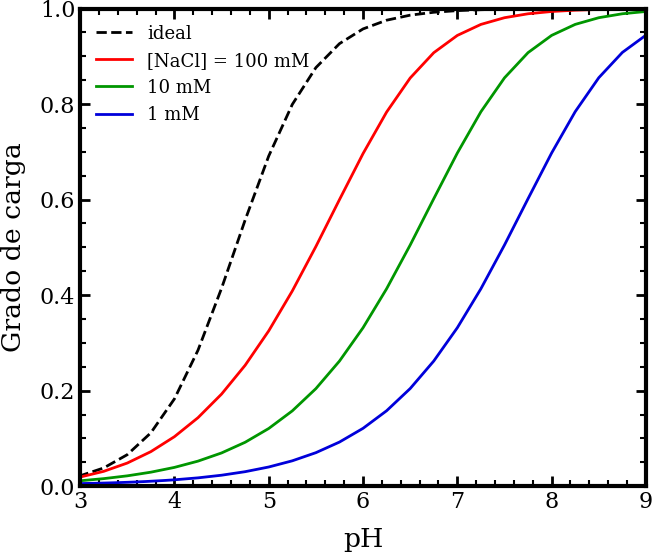
\includegraphics[width=0.9\textwidth]{Figures/graph-film/charge_degree-film.png}
    \caption{Grado de carga del gel como funci\'on del pH. Grado de carga para un monomero aislado en presentado en curva a rayas, se compara paa concentraciones de sal diferente, a mayor concentraci\'on salina m\'as nos acercamos al sistema ideal.}
    \label{fig:degree-film}
\end{figure}



A un pH dado, es significativamente menos probable que se cargue una unidad ácida de la red de lo que se espera según las consideraciones ideales. La concentración de sal de la solución resulta ser una variable crítica que modula este comportamiento de regulación de carga. A una salinidad relativamente alta, se encuentran concentraciones significativas de los contraiones dentro del hidrogel, lo que da como resultado el apantallamiento de interacciones electrostáticas, que volviendose de corto alcance. Esta apantallamiento de repulsiones dentro de la red permite que el polímero aumente su grado de carga para reducir la energía libre descripta por el equilibrio ácido-base de los segmentos de la cadena. El aumento en la salinidad genera una protonación que se aproxima al comportamiento ideal. En condiciones de baja salinidad, por otro lado, aumenta el costo entrópico de confinar iones dentro del hidrogel. Solo se encuentran los suficientes contraiones dentro de la red para neutralizar la carga eléctrica del polímero. Bajo tales condiciones, el efecto de apantallamiento de los iones de sal se debilita y las interacciones electrostáticas se vuelven efectivamente de mayor alcance. Como resultado, la red se carga menos para prevenir o reducir las repulsiones dentro de la red.

Otro aspecto a considerar es el pH local el cual es definido en la posición espacial \textbf{r}  utilizando la concentración local de protones:
\begin{equation}
    pH(r) = -\log_{10}([H^+](r))
    \label{eq:pH-local}
\end{equation}
Una baja disociaci\'on (un nivel de protonaci\'on alto) de las unidades \'acidas del pol\'imero puede explicarse en terminos del pH local dentro del material. Se define el $pH_{gel}$ como el promedio del pH local dentro del film. Resultados previos han mostrado que esta cantidad esta bien definida \addcite. En esta secci\'on enfatizaremos la importancia de estos dos terminos $pH_{gel}$ y $pH(r)$ por la informaci\'on que proveen: el estado de carga/protonaci\'on de las unidades titulables en la red polim\'erica. 

Haciendo uso de la eq. \ref{eq:diso} es posible calcular el grado de disoción de la estructura polimérica. El uso del $pH_{gel}$ es indispensable para cuanod el pH es distinto al  del seno de la solución \addcite. El mismo procedimiento se realiza para calcular el estado de protonación local de las unidades titulables de las especies que se adsorben en el film (ver figura \ref{fig:protein-charge}).

\begin{figure}
    \centering
    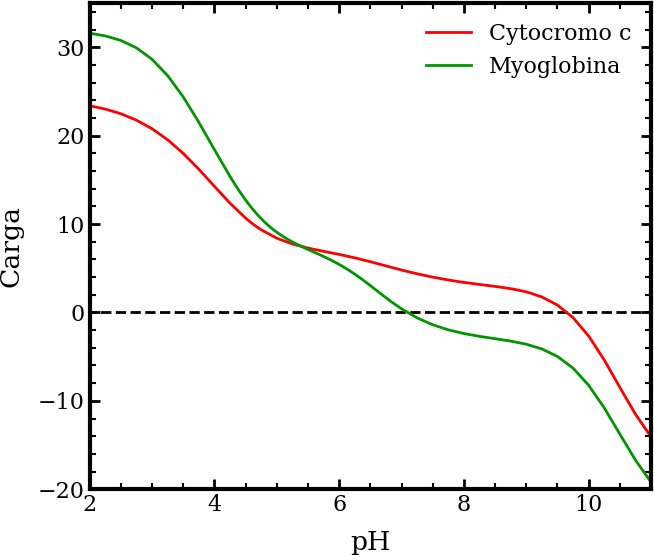
\includegraphics[width=0.9\textwidth]{Figures/graph-film/carga-proteinas.png}
    \caption{N\'umero de carga de las proteinas cytocromo c y myoglobina como  funci\'on del pH en el seno de la soluci\'on (bulk). La l\'inea a trazos muestra el cambio en el signo de la carga.}
    \label{fig:protein-charge}
\end{figure}



Sin embargo, aunque esto parece simplificar el problema de establecer la carga neta de cualquier especie dentro del material, incluida la red polimérica y las proteínas adsorbidas, determinar los cambios en el pH local tiene la misma complejidad que el problema original (es decir, determinar la carga de la la red). El pH local que se establece dentro del material, así como su valor en la interfaz entre el polímero y la solución acuosa, es el resultado de la compleja interacción entre la organización molecular, los equilibrios químicos y las interacciones físicas que determinan el equilibrio termodinámico a las condiciones impuestas externamente (pH, concentración de sal). Por ejemplo, la figura \ref{fig:pH-local} muestra el pH dentro de una película de hidrogel de PMAA como una función del pH  y la concentración de sal, calculado usando teor\'ia molecular.

\begin{figure}
    \centering
    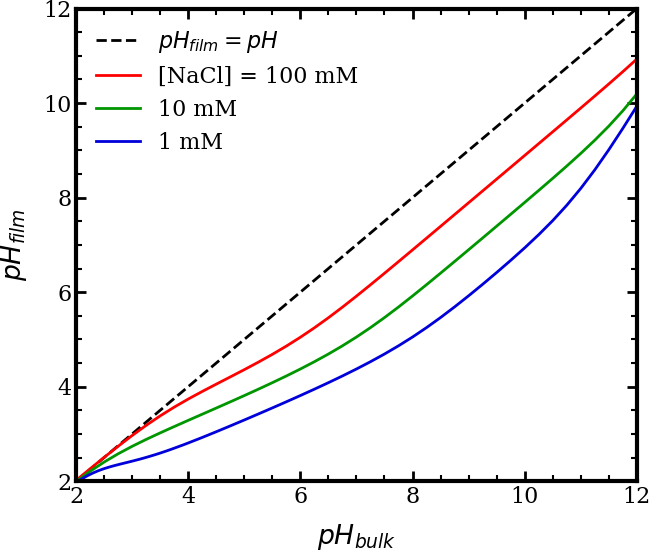
\includegraphics[width=0.9\textwidth]{Figures/graph-film/pH-local.png}
    \caption{pH local del gel como funci\'on del pH en el seno de la soluci\'on (bulk). Cada curva corresponde a una concentraci\'on de sal diferente.}
    \label{fig:pH-local}
\end{figure}

\subsection{Adsorci\'on}
Como se mencion\'o al incio de este capitulo... poder usar estos sistemas de hidrogeles como carries de adsrobatos de utilidad terap\'eutica.
Para ello nos valdremos de la teor\'ia molecular y haciendlo uso de ciertas prote\'inas modelo como lo son el cytocromo c y la myoglobina. estas dos presentan gran estabilidad en un amplio rango de pH y recientemente se ha  investigado la termodinámica  de su adsorci\'on en sistemas polim\'ericos similares. \addcite

Para cuantificar la cantidad de adsrobato adsrobido en el hidrogel utilizamos la expresi\'on:

\begin{align}
\Gamma = \int_V {dr(\rho(r) -\rho_{bulk}}  
\label{adsor}
\end{align}

en donde $\rho(r)$ y $\rho_{bulk}$ son las densidades del  locales y en el seno de la soluci\'on del adsorbato respectivamente, V es el volumen de la soluci\'on. 
Esta adsorción proporciona la masa  en un volumen particular por exceso de la contribución del bulk. En particular dentro del hidrogel, $\Gamma$ proporciona la cantidad de adsorbato en exceso dentro del material, recibiendo también contribuciones de la interfaz de solución de polímero.

Para estas proteínas, la adsorción es una función no monotónica del pH de la solución (ver Figura \ref{fig:ad-pro}). A pH bajo, estas proteínas tienen una carga alta y positiva, pero la red de poliácidos solo está débilmente ionizada (véanse las Figuras \ref{fig:degree-film} y \ref{fig:protein-charge}). A un pH suficientemente alto, por otro lado, el polímero está fuertemente cargado negativamente, pero las proteínas tienen una carga débilmente positiva o incluso negativa. Bajo tales condiciones (muy) ácidas o alcalinas, las interacciones electrostáticas son débilmente atractivas o repulsivas. No hay fuerza impulsora para la adsorción. A valores de pH intermedios, por el contrario, donde tanto la proteína como la red de poliácidos tienen cargas fuertes y opuestas, se produce una adsorción significativa con un máximo necesario en tales condiciones.

La adsorción de proteínas depende críticamente de la concentración de sal de la solución. Este comportamiento se ilustra en la figura \ref{fig:ad-pro} que muestra la adsorción de citocromo c  y mioglobina en una película de hidrogel de PMAA. La disminución de las concentraciones de sal mejora la adsorción y amplía el rango de pH de la adsorción. Por ejemplo, ambos paneles de la \ref{fig:ad-pro} muestran una disminución de aproximadamente un orden de magnitud en la adsorción cuando se comparan soluciones de NaCl 1 mM y 10 mM. El pH de máxima adsorción también depende de la salinidad de la solución. Este comportamiento es aún más interesante cuando se considera que una concentración de sal más baja conduce a una red con carga más débil, como describimos con anterioridad. En otras palabras, la red de polímero con carga más débil, a medida que disminuye la concentración de sal, más proteína es adsorbida. Esta última afirmación es cierta en las concentraciones de proteína ($10 \mu M$) y sal de la figura \ref{fig:ad-pro}, donde la adsorción solo modifica ligeramente el grado de carga de la red.

Esta dependencia de la adsorción de la concentración de sal tiene tres razones principales: en primer lugar, existe la protección de las atracciones electrostáticas de la red de proteínas por parte de los iones de sal. Cuanto menor sea la concentración de sal, más débil será la detección de las interacciones proteína-red, lo que mejora la adsorción. En segundo lugar, a medida que la concentración de sal disminuye, el pH dentro de las gotas de hidrogel (a un pH general dado). Esto implica que las proteínas adsorbidas tienen una carga más positiva tras la adsorción (a medida que disminuye ½NaCl?). En tercer lugar, la ganancia entrópica de la liberación de contraiones de la red de polímeros es mayor a medida que disminuye la concentración de sal, lo que también favorece la adsorción de proteínas.



\begin{figure}
    \centering
    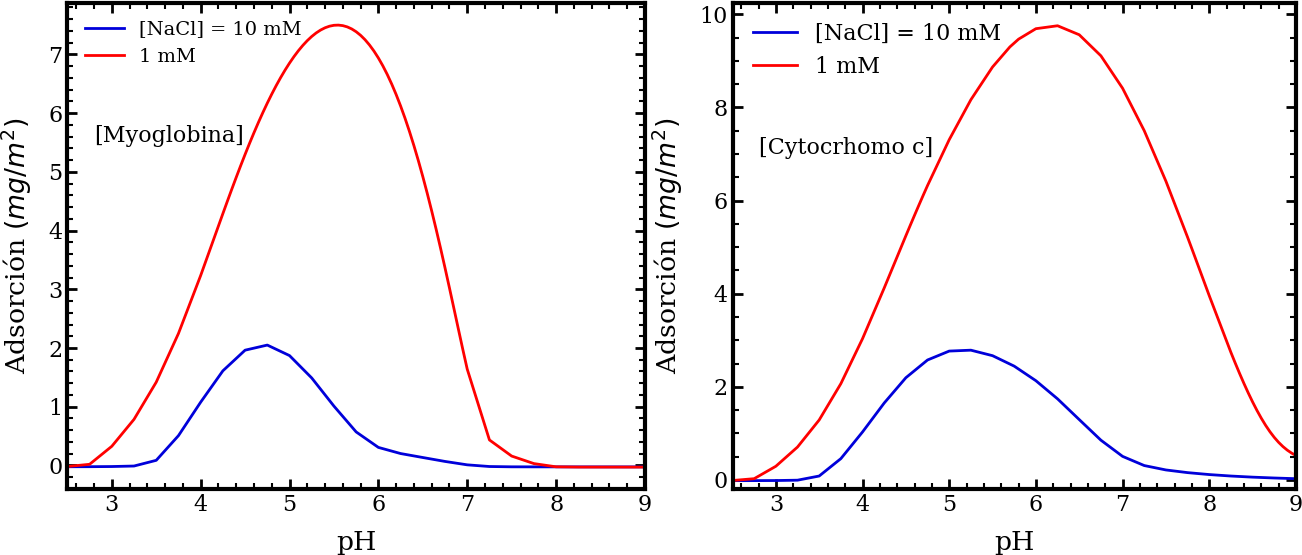
\includegraphics[width=0.99\textwidth]{Figures/graph-film/ad-proteins.png}
    \caption{Adsorci\'on de proteinas: cytocromo c y myoglobina en panel A y B respectivamente. La concentraci\'on de los adsorbatos es $10 \mu M$}
    \label{fig:ad-pro}
\end{figure}

% Chapter 3

\chapter{Geles polim\'ericos} % Main chapter title

\label{Chapter-geles} % For referencing the chapter elsewhere, use \ref{Chapter1} 

%----------------------------------------------------------------------------------------

% Define some commands to keep the formatting separated from the content 
\newcommand{\keyword}[1]{\textbf{#1}}
\newcommand{\tabhead}[1]{\textbf{#1}}
\newcommand{\code}[1]{\texttt{#1}}
\newcommand{\file}[1]{\texttt{\bfseries#1}}
\newcommand{\option}[1]{\texttt{\itshape#1}}

%----------------------------------------------------------------------------------------




\section{Introducci\'on}

Los micro-nanogeles polim\'ericos son sistemas polim\'ericos que presentan una estructura tridimensional en forma de red. Estos geles se forman mediante la reticulaci\'on de pol\'imeros (o copol\'imeros), lo que da lugar a una matriz de pol\'imero tridimensional que puede retener grandes cantidades de agua o solventes.
Estos sitemas han demostrado ser de gran inter\'es en una amplia gama de aplicaciones, incluyendo el encapsulado y la liberaci\'on  de fármacos, la ingenier\'ia de tejidos y la bioimagen.
Los geles representan una plataforma vers\'atil y prometedora para diversas aplicaciones biom\'edicas. Su capacidad para retener agua y solventes, su tama\~no nanom\'etrico y su capacidad de funcionalizaci\'on los convierten en sistemas atractivos para la entrega de f\'armacos

\textcolor{red}{falta enganche}

En este cap\'itulo mostramos el desarrollo de una teor\'ia de equilibrio de dos fases y realizamos una investigaci\'on sistem\'atica del comportamiento termodin\'amico de microgeles compuestos de copol\'imeros aleatorios de NIPAm y un comon\'omero \'acido (MAA).
Este modelo describe la qu\'imica f\'isica detr\'as de todos los fen\'omenos de hinchamiento del microgel impulsado por el pH, la dependencia no monot\'onica del tama\~no de part\'icula de la concentraci\'on de sal y el colapso de la red al aumentar la temperatura por encima del VPTT.
Las predicciones que mostramos brindan una imagen clara de los efectos de la composici\'on de la soluci\'on (pH, concentración de sal) y la qu\'imica del pol\'imero (contenido de MAA, grado de entrecruzamiento) en el VPT.
Tambi\'en investigamos las mejores condiciones para la encapsulaci\'on de doxorrubicina y daunorrubicina dentro de estos microgeles.
Los c\'alculos  ac\'a mostrados son espec\'ificos para el \'acido metacr\'ilico con $pKa = 4,65$, pero el comportamiento fisicoqu\'imico informado puede describir cualitativamente una variedad de microgeles basados en NIPAm que se han modificado con otros mon\'omeros \'acidos que tienen diferente pka y diferente solubilidad a pH bajo.

El modelo y nivel de teor\'ia usado en este cap\'itulo corresponde a un sitema de dos fases, del tipo Donnan \addcite, en el cual la fase polim\'erica es considera homogenea. La fase soluci\'on con la que se encuentra en contacto contiene los iones y adsorbatos lso cuales pueden permear en la fase polim\'erica. En la cambio el gel no puede pasar a la fase soluci\'on. 
El sistema termodinamicamente hablando corresponde a un sistema semi-gran canonico que incluye todas las los terminos energeticos necesarios para una descripci\'on detallada del mismo. 
En las siguientes secciones se har\'a rese\~na sobre las ecuaciones que describen la fisicoqu\'imica del sistema. 

\subsection{Teor\'ia: Fase Microgel}\label{sec:gel:theory}
%%%%%%%%%%%%%%%%%%%%%%%%%%%%%%%%%%%%%%%%%%%%%%%%%%%%%%%%%%%%%%%%%%%%%


Consideremos un modelo de dos fases: un microgel de poli(NIPAm-\emph{co}-MAA) (P(NIPAm-MAA)) (la fase $1$, denotada por $MG$) en contacto con una soluci\'on acuosa ( fase $2$, denotada por $s$).
Externamente, podemos controlar la temperatura $T$, el pH y la concentraci\'on de sal de esta soluci\'on, lo que da como resultado que el microgel tenga un radio $R$ y un volumen $V=\frac{4}{3}\pi R^3$.
El potencial termodin\'amico cuyo m\'inimo produce las condiciones de equilibrio dentro de la fase de microgel es un  potencial semi gran can\'onico, $\Omega_{MG}$.
%
\begin{align}
    \begin{aligned}
       \Omega_{MG}=& -TS_{mez} + F_{qca,MAA} +  F_{ela}\\
       & + U_{elec}+  U_{ste} + U_{VdW} -{\sum_{\gamma}
        {\mu_\gamma N_\gamma}}
    \end{aligned}
    \label{eq:gel:free-energy-implicit}
\end{align}
%

\noindent En donde $S_{mez}$ es la entropí\'ia de traslaci\'on (mezcla) de las especies libres en la fase de microgel: mol\'eculas de agua ($w$), hidronio ($H_3O^+$) e iones de hidr\'oxido ($OH^-$ ), y cationes de sal ($+$) y aniones ($-$).
Hemos considerado una sal monovalente, $KCl$,  completamente disociada en iones de potasio y cloruro.

\begin{align}
-\frac{S_{mez}}{k_B}	= \sum_{\gamma} \rho_\gamma\left(\ln\left(\rho_\gamma v_w\right) -1 + \beta\mu^0_\gamma\right) 
\end{align}

\noindent en donde  $\beta=\frac{1}{k_BT}$ , $T$ es la temperatura del sisteman y  $k_B$ es la constante de Boltzmann.
La densidad num\'erica de la especie $\gamma$ es $\rho_\gamma$ y $\mu^0_\gamma$ es su potencial qu\'imico est\'andar,  $v_w$ es el volumen de una mol\'ecula de agua.

$F_{qca,MAA}$ es la energ\'ia química libre que describe la protonaci\'on de equilibrio de las unidades de MAA.


\begin{align}
	\beta F_{qca, MAA} =  \frac{\phi_{MAA}}{v_{MAA}} \left[f(\ln f+ \beta\mu^0_{MAA^-}) +(1-f)(\ln (1-f)+\beta\mu^0_{MAAH})\right]
\end{align}


\noindent donde $\phi_{MAA}$ es la fracci\'on de volumen que ocupan estos segmentos, $v_{MAA}$ es el volumen de este segmento, y $f$ es el grado de disociaci\'on del mismo. 
La fracci\'on de volumen de los segmentos MAA cargados es $f\phi_{MAA}$, y la de las unidades protonadas (o sin carga) es $(1-f)\phi_{MAA}$.
Los potenciales qu\'imicos est\'andar son $\mu^0_{MAA^-}$ y $\mu^0_{MAAH}$ para las especies desprotonadas(cargadas) y protonadas, respectivamente.
Utilizamos el t\'ermino segmento para identificar las unidades qu\'imicas que componen las cadenas polim\'ericas (MAA y NIPAm).


$F_{ela}$ es la energ\'ia libre el\'astica que explica la libertad conformacional de la red polim\'erica.

\begin{align}
	\beta F_{ela} = \dfrac{3}{2}\dfrac{N_{seg}}{n_{ch} V}\left[\left(\dfrac{R}{R_0}\right)^2 - \ln\dfrac{R}{R_0} -1\right]
\end{align}

Esta expresi\'on se describe en \cite{moncho-jorda2016a} y proviene del modelo de elasticidad del caucho,
donde $N_{seg}$ es el n\'umero total de segmentos en la red de pol\'imero y $n_{ch}$ es el n\'umero de segmentos por cadena de pol\'imero o \emph{longitud de cadena}.
La constante de elasticidad en esta energ\'ia es proporcional al cociente $\dfrac{N_{seg}}{n_{ch}}$, que representa el n\'umero (total) de cadenas de pol\'imero en el microgel.
El radio del microgel seco es $R_0$, lo que satisface con la expresi\'on:

%
%
\begin{align}
	\begin{aligned} 
		\dfrac{4}{3}\pi R_0^3=V_0&=N_{seg}\Big( x_{MAA} v_{MAA}\\
		&\qquad+x_{NIPAm} v_{NIPAm}\Big)
	\end{aligned}
\end{align}


\noindent donde $V_0$ es el volumen de la part\'icula seca; $x_{MAA}$ y $x_{NIPAm}$ son la fracci\'on de los segmentos MAA y NIPAm, respectivamente.
Entonces, el n\'umero total de segmentos MAA es $x_{MAA}N_{seg}$ y el de unidades NIPAm es $x_{NIPAm}N_{seg}$, cada uno con un volumen $v_{NIPAm}$.
Los microgeles que consideramos aqu\'i satisfacen $x_{NIPAm}=1-x_{MAA}$.



$U_{elec}$ y $U_{ste}$ representan respectivamente las interacciones electrost\'aticas y las repulsiones est\'ericas.

\begin{align}
	  \beta U_{elec} =\left(\sum_{\gamma } {\rho_\gamma q_\gamma + f\dfrac{\phi_{MAA}}{v_{MAA}}q_{MAA}}\right)\beta\psi_{MG}
\end{align}

\noindent donde $q_\gamma$ y $q_{MAA}$ son la carga el\'ectrica de las moléculas $\gamma$ y los segmentos MAA, respectivamente.
El potencial electrost\'atico dentro de la fase de microgel es $\psi_{MG}$. Fuera de esta fase el potencial es nulo $\psi_s = 0$

En donde se impone una restriccio\'on de electroneutralidad del microgel, que puede expresarse como:
%
%
\begin{align}
	\begin{aligned}
		\sum_{\gamma  } \rho_\gamma q_\gamma + f\frac{\phi_{MAA}}{v_{MAA}}q_{MAA}=0
	\end{aligned}
	\label{eq:gel:charge-neutrality}
\end{align}

Las interacciones stericas se incorporan como una segunda restricci\'on al sistema, la cual consiste en que  el volumen del microgel est\'a completamente ocupado por los segmentos de la red y las especies quí\'icas libres.

%
\begin{align}
	\begin{aligned}
		\sum_{\gamma } \rho_\gamma v_\gamma  + \phi_{MAA} + \phi_{NIPAm} = 1
	\end{aligned}
	\label{eq:gel:packing}
\end{align}



\noindent donde $v_\gamma$  es el volumen molecular de la especie $\gamma$, y la fracci\'on de volumen de cada componente de la red son: 
%
%
\begin{align}
	\phi_{MAA}&=N_{seg}\dfrac{x_{MAA}v_{MAA}}{\frac{4}{3}\pi R^3}\\
	\phi_{NIPAm}&=N_{seg}\dfrac{x_{NIPAm}v_{NIPAm}}{\frac{4}{3}\pi R^3}
\end{align}



$U_{VdW}$ es la contribuci\'on que describe las interacciones efectivas pol\'imero-disolvente; para este trabajo hemos realizado la siguiente aproximaci\'on: 
\begin{align}
	U_{VdW} = U_{NIPAm-w} + U_{MAA-w}
\end{align}
\noindent en donde $U_{NIPAm-w}$ incorpora la transici\'on hidrofílica-hidrof\'obica de NIPAm al aumentar la temperatura por encima de su temperatura de transici\'on cr\'itica. 
Del mismo modo $U_{MAA-w}$ hace cuenta de la interacci\'on entre los segmentos de MAA y agua.
Los resultados presentes en este cap\'itulo consideran a los segmentos de $MAA$ completamente hidrofilicos y por tanto $U_{MAA-w} = 0$

\begin{align}
	\beta U_{VdW} = U_{NIPAm-w} = \chi (T, \phi_{NIPAm})\rho_w \phi_{NIPAm}
\end{align}


Este  t\'ermino explica la respuesta de PNIPAm a los cambios de temperatura a trav\'es de un par\'ametro de interacci\'on pol\'imero solvente, $\chi$, que depende de la temperatura y la fracci\'on de volumen de NIPAm, $\phi_{NIPAm}$.
Seg\'un  \citet{afroze2000}, este par\'ametro de Flory-Huggins se puede expresar como:
%
%


\begin{align}
	\begin{aligned}
		\chi (T, \phi_{NIPAm}) &=g_0(T) +g_1(T)\phi_{NIPAm} \\
		&~+ g_2(T)\phi_{NIPAm}^2
	\end{aligned}
\end{align}

\noindent con
%
%
\begin{align}
	\begin{aligned} 
		g_k(T)=g_{k0} + \frac{g_{k1}}{T} + g_{k2}T
	\end{aligned}
\end{align}


\noindent para  $k=0,1,2$, los coeficinetes son: $g_{00}= -12.947$, $g_{02}=0.044959\,$K$^{-1}$, $g_{10}= 17.920$, $g_{12}= -0.056944$\,K$^{-1}$, $g_{20}= 14.814$, $g_{22}= -0.051419$\,K$^{-1}$  y $g_{k1}\equiv 0$ \cite{afroze2000}




Finalmente, la suma sobre  $\gamma$ expresa el equilibrio qu\'imico con la fase de soluci\'on, donde $\mu_\gamma$ y $N_\gamma$ son el potencial qu\'imico y el n\'umero de mol\'eculas de la especie $\gamma$, respectivamente.
Aqu\'i, el subíndice $\gamma$ identifica  las especies qu\'imicas libres, $\gamma \in \left\{ w, H_3O^+, OH^-, +,- \right\}$.
Hay que tener en cuenta que $\Omega_{MG}$ es un potencial semi-gran can\'onico porque la fase de microgel puede intercambiar cada una de estas mol\'eculas con la fase de soluci\'on, mientras que la red de pol\'imero está confinada dentro de la primera.


\begin{align}
	\sum_\gamma N_\gamma \mu_\gamma = \sum_{\gamma }{\rho_\gamma\beta\mu_\gamma}
	+ \beta\mu_{H^+}(1-f)\dfrac{\phi_{MAA}}{v_{MAA}}
\end{align}

Esta contribuci\'on muestra el equilibrio qu\'imico entre el microgel y la fase de soluci\'on, donde el segundo t\'ermino representa a los protones asociados a unidades de MAA;
a saber, $\mu_{H^+}\equiv\mu_{H_3O^+}$ se conjuga con el n\'umero total de protones,
$N_{H_3O^+}+N_{MAAH}=V\left(\rho_{H_3O^+}+(1-f)\dfrac{\phi_{MAA}}{v_{MAA}}\right)$.


La forma expl\'icita del potencial termodin\'amico es:




%
\begin{align}
\begin{aligned}
\beta&\frac{\Omega_{MG}(R)}{V}=\\& ~ \sum_{\gamma} \rho_\gamma\left(\ln\left(\rho_\gamma v_w\right) -1 + \beta\mu^0_\gamma\right) \\
& + \frac{\phi_{MAA}}{v_{MAA}} \left[f(\ln f+ \beta\mu^0_{MAA^-})\right.\\
&\qquad\left.+(1-f)(\ln (1-f)+\beta\mu^0_{MAAH})\right] \\
%
& + \dfrac{3}{2}\dfrac{N_{seg}}{n_{ch} V}\left[\left(\dfrac{R}{R_0}\right)^2 - \ln\dfrac{R}{R_0} -1\right] \\
%
& +  \left(\sum_{\gamma } {\rho_\gamma q_\gamma + f\dfrac{\phi_{MAA}}{v_{MAA}}q_{MAA}}\right)\beta\psi_{MG}\\
%
& +\beta\pi_{MG} \left[ \sum_{\gamma } \rho_\gamma v_\gamma  + \phi_{MAA} + \phi_{NIPAm} -1 \right] \\
%
& + \chi (T, \phi_{NIPAm})\rho_w \phi_{NIPAm} \\
%
& -\sum_{\gamma }{\rho_\gamma\beta\mu_\gamma}
 -\beta\mu_{H^+}(1-f)\dfrac{\phi_{MAA}}{v_{MAA}}\\
%
%
\end{aligned}
\label{eq:gel:free-energy}
\end{align}




\noindent En donde $\pi_{MG}$ es la presi\'on osm\'otica de la fase de microgel, introducido como un multiplicador de Lagrange para imponer la restricci\'on de incompresibilidad, ec. \ref{eq:gel:packing}.


Nuestro potencial termodin\'amico esta explicitamente en funci\'on de las densidades de todas las especies, el grado de carga del MAA y el radio del microgel, $\Omega_{MG}(R)\equiv\Omega_{MG}(\{\rho_\gamma\},f,R)$.
Para obtener las expresiones de $\{\rho_\gamma\}$ y $f$ de tal forma que sean consistentes con el equilibrio termodin\'amico, minimizamos $\Omega_{MG}$ respecto a estas cantidades, y  sujeto a las restricciones ec. \ref{eq:gel:packing} y ec. \ref{eq:gel:charge-neutrality}; dicho procedimiento conduce a: 
%
%
\begin{align}
\rho_\gamma v_w &= a_\gamma \exp(-\beta\pi_{MG}v_\gamma -\beta\psi_{MG}q_{\gamma})\\
\frac{f}{1-f}&= \frac{K^0_{MAA}}{a_{H^+}}\exp(-\beta\psi_{MG}q_{MAA})\label{eq:gel:fcharge}
\end{align}

\noindent donde $a_\gamma = e^{\beta\mu_\gamma-\beta\mu_\gamma^0}$ es la actividad de la especie $\gamma$. 
La constante de equilibrio termodin\'amico que describe la protonaci\'on/desprotonaci\'on MAA es
%
%
\begin{align}
K^0_{MAA}= e^{\beta\mu^0_{MAAH}-\beta\mu^0_{MAA}-\beta\mu^0_{H^+}}
\end{align}

\noindent Esta cantidad es posible calcularla directamente a partir del pKa del \'acido.


Si se considera  un valor de  $R$, las \'unicas inc\'ognitas restantes para determinar $\Omega_{MG}(R)$ son la presi\'on osm\'otica, $\pi_{MG}$ y el potencial electrost\'atico, $\psi_{MG}$.
Estas dos cantidades se pueden calcular resolviendo num\'ericamente la incompresibilidad y la electroneutralidad de la fase de microgel, ec. \ref{eq:gel:packing} y ec. \ref{eq:gel:charge-neutrality}, respectivamente.
Para resolver estas ecuaciones utilizamos un m\'etodo h\'ibrido de Powell sin jacobiano y un c\'odigo FORTRAN desarrollado internamente.
En resumen, es posible calcular la variaci\'on de energ\'ia potencial respecto del radio del microgel $R$, y con ello calcular el valor del radio \'optimo del gel para unas condiciones dadas( pH, temperatura, concentraci\'on de sal). Esto se ilustra en la secci\'on \ref{sec:gel:minimi}.

Todas las dem\'as cantidades involucradas en el c\'alculo de $\Omega_{MG}(R)$ son valores de  entradas, incluidas las propiedades de las diferentes especies qu\'imicas consideradas, que se resumen en la tabla \ref{table:gel:molecules}.
Usamos $pK_w=14$ para describir el equilibrio de disociaci\'on del agua.
Las actividades de todas las especies qu\'imicas libres se pueden calcular a partir de la concentraci\'on de estas mol\'eculas en la fase de soluci\'on, como se analiza a continuaci\'on.


\begin{table}
	\centering
%\small
%\begin{tabular}{lcS[table-format=-1]S[table-format=0.3]}
\begin{tabular}{|lccc|}
    \hline
    {Species} & {$pKa$} & {$q$ ($e$)} & {$v$ ($\text{nm}^3$)} \\
      \hline
$H_2O\,(w)$ & ~ & ~ & 0.03\\
$H_3O^+$ & ~ & +1 & 0.03\\
$OH^-$ & ~ & -1 & 0.03\\
$K^+\,(+)$ & ~ & +1 & 0.04\\ 
$Cl^-\,(-)$ & ~ & -1 & 0.047\\
$MAA$ & 4.65 & -1$^\ast$ & 0.09\\
$NIPAm$ & ~ & ~ & 0.12\\
    \hline
  \end{tabular}
 \caption{Propiedades moleculares de las diferentes especies qu\'imicas consideradas.
 	\footnotesize ($^\ast$Para las especies desprotonadas).}
\label{table:gel:molecules} 
\end{table}


%%%%%%%%%%%%%%%%%%%%%%%%%%%%%%%%%%%%%%%%%%%%%%%%%%%%%%%%%%%%%%%%%%%%%
\subsection{Fase soluci\'on}\label{sec:gel:fase-solucion}
%%%%%%%%%%%%%%%%%%%%%%%%%%%%%%%%%%%%%%%%%%%%%%%%%%%%%%%%%%%%%%%%%%%%%

En la soluci\'on, el potencial termodin\'amico es:
%
%
\begin{align}
\begin{aligned}
\beta&\frac{\Omega_s}{V}=\\& \sum_{\gamma   } {\rho^s_\gamma\left(\ln(\rho_\gamma^sv_w) -1 + \beta\mu_\gamma^0 - \beta\mu_\gamma\right)} \\
& +\beta\pi_{s} \left[ \sum_{\gamma } \rho_\gamma v_\gamma + \rho_a \sum_\lambda n_\lambda v_\lambda -1 \right] \\
\end{aligned}
\label{eq:gel:bulk}
\end{align}

\noindent el subindice  $s$  indica las densidades en la fase soluci\'on.
Al escribir la ec. \ref{eq:gel:bulk}, hemos considerado un volumen de referencia igual al del microgel, $V$, y se ha considerado, como se mencion\'o con anterioridad, cero el potencial electrost\'atico en la fase de soluci\'on.
Adem\'as en la ultima l\'inea de la ecuaci\'on \ref{eq:gel:bulk} se ha incorporado la restricci\'on para la incompresibilidad del sistema, con $pi_s$ como la presi\'on osm\'otica en la fase soluci\'on.

Una vez que se establece la composición de la soluci\'on (pH y concentraci\'on de sal), conocemos las densidades de todas las especies qu\'imicas en esta fase, que deben satisfacer tanto las restricciones de incompresibilidad como de neutralidad de carga:
%
%
\begin{align}
\sum_{\gamma  } \rho_\gamma^s v_\gamma  &=1\label{eq:gel:bulk-packing}\\
\sum_{\gamma  } \rho_\gamma^s q_\gamma  &=0
\end{align}

\noindent con
%
%
\begin{align}
\rho_\gamma^s v_w= a_\gamma \exp(-\beta\pi_s v_\gamma)
\label{eq:gel:bulk-electroneutrality}
\end{align}



\noindent para $\gamma \in \left\{ w, H_3O^+, OH^-, +,- \right\}$, donde $\pi_s$ es la presi\'on osm\'otica de la fase de soluci\'on introducida como un multiplicador de Lagrange por la ecuaci\'on \ref{eq:gel:bulk-packing}.
Al conocer $\pi_s$, podemos determinar las actividades de todas las especies qu\'imicas libres, y con las mismas resolver el sistema de la fase microgel.
Los resultados de la minimizaci\'on de la energ\'ia con un dado valor de R es presentada en la siguiente secci\'on.

\subsection{Minimizaci\'on gr\'afica}\label{sec:gel:minimi}
%%%%%%%%%%%%%%%%%%%%%%%%%%%%%%%%%%%%%%%%%%%%%%%%%%%%%%%%%%%%%%%%%%%%%

\begin{figure*}[!htb]
\centering
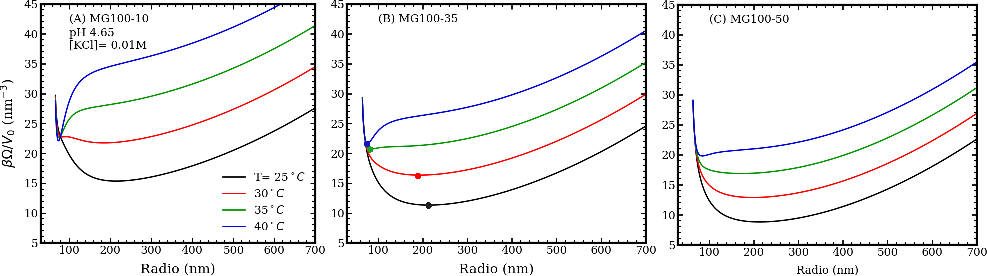
\includegraphics[width=1.\linewidth]{Figures/graph-gel/graph-min.pdf}
\caption{Potencial termodin\'amico en funci\'on del radio del microgel a diferentes temperaturas, $pH~4.65$ y $cs=10^{-2}M$.
	Cada panel corresponde a un microgel MG100 diferente (longitud de cadena, $n_{ch}=100$) con $10\%$ (A), $35\%$ (B) y $50\%$ (C) MAA.
	Las curvas presentan el potencial termodin\'amico en exceso de la contribuci\'on de la soluci\'on, $\Omega=\Omega_{MG}-\Omega_s$, en algunas unidades convenientes, donde $V_0=\frac{4}{3}\pi R_0^3$ es el volumen de la part\'icula polim\'erica seca.
	En el panel B, los puntos  marcan el radio \'optimo para cada temperatura, que es el m\'inimo local/global de la curva correspondiente (ver tabla \ref{table:gel:optimal-R}).}
\label{fig:gel:graph-min}
\end{figure*}

Como mencionamos en la secci\'on \ref{sec:gel:theory} es posible determinar completamente la energ\'ia libre de la fase de microgel para cualquier $R$ dado.
Las variables independientes en este c\'alculo son la temperatura, el pH y la concentraci\'on de sal de la soluci\'on en contacto con la fase microgel.
El n\'umero de segmentos en la red de pol\'imero $N_{seg}$, la longitud de la cadena $n_{ch}$ y la fracci\'on de segmentos MAA, $x_{MAA}$, caracterizan completamente a nuestro microgel, es decir son variables de entrada pre-establecidas.


Consideramos microgeles con $N_{seg}=10^7$ segmentos y $n_{ch}=50$, $100$ y $200$, que tienen $x_{MAA}=0,1$, $0,35$ o $0,5$.
En esta primera instancia evaluamos el efecto de aumentar o reducir la cantidad de mon\'omero \'acido con respecto a los microgeles de poli(NIPAm-\emph{co}-MAA) que tienen $35\%$ MAA.

Estos microgeles est\'an etiquetados como MG$n_{ch}$-$p_{MAA}$, donde $p_{MAA}$ es el porcentaje de MAA.
Por ejemplo, MG100-10 corresponde a un  microgel con $n_{ch}=100$ y $x_{MAA}=0,1$.


Para determinar el tama\~no del microgel para un conjunto dado de condiciones, recurrimos a una minimizaci\'on gr\'afica del mismo.
Para cada conjunto de condiciones (pH, sal y $T$), obtenemos la energ\'ia $\Omega(R)=\Omega_{MG}(R)-\Omega_{s}(R)$. En esta expresi\'on obtenemos el potencial termodin\'amico en exceso de la contribuci\'on energ\'etica de la soluci\'on.
Con ella podemos encontrar el $R_{opt }$, siedo este el radio \'optimo, tal que la curva tenga un m\'inimo local (y global).
Como ejemplo, este procedimiento se ilustra en la figura \ref{fig:gel:graph-min} para microgeles MG100.
Los resultados obtenidos de la minimizaci\'on de las curvas figura \ref{fig:gel:graph-min} se resumen en la tabla \ref{table:gel:optimal-R}.

\begin{table}[!htb]
\centering
\small
  \begin{tabular}{|lccccc|}
   \hline %\multirow{2}{*}{MG100} & 
    %  \multicolumn{4}{c}{Opt. Radius (nm)(MG100)} \\
    	&&   Radio \'optimo (nm)(MG100) & && \\
    	\hline
      & {25 $^\circ C$} & {30 $^\circ C$} & {35 $^\circ C$} & {40 $^\circ C$} & {Gel seco, $R_0$} \\
      \hline
    10\% MAA & 215 &  184 &  75  &  74 & 65\\
    35\% MAA &  213 &  193 &  84 & 76 & 64\\
    50\% MAA &  213 & 199 &  172 & 85 & 63\\
    \hline
  \end{tabular}
 \caption{Minimizaci\'on de las curvas de la  figura \ref{fig:gel:graph-min}.
 	Esta tabla resume los radios \'optimos de tres microgeles MG100 a diferentes temperaturas, $pH\,4.65$ y $[KCl]=10^{-2}M$.}
\label{table:gel:optimal-R} 
\end{table}


\subsection{Absorci\'on}\label{sec:gel:adsorcion}
%%%%%%%%%%%%%%%%%%%%%%%%%%%%%%%%%%%%%%%%%%%%%%%%%%%%%%%%%%%%%%%%%%%%%

Nuestro objetivo es poder utilizar estos microgeles como dispositivos inteligentes, entre los que se destaca su uso como trasnportadores de mecidamentos. Para ello es necesario analizar su factibiliad de su absorci\'on de algunas drogas terapeuticas. En el presente cap\'itulo realizamos el an\'alisis usando como droga modelo a la Doxorubicina y un derivado de ella: Daunorubicina. Ambas drogas muy fuertemente empleadas en tratamientos anticancerigenos. 

Para describir la absorci\'on de un analito a la fase de microgel,
al potencial termodin\'amico de la ec. \ref{eq:gel:free-energy} se le adicionan los siguientes t\'erminos:
%
%
%
\begin{align}
\begin{aligned}
\beta&\frac{\Omega_{MG}(R)}{V}= \cdots\\&+ \rho_a\left(\ln\left(\rho_a v_w\right) -1 + \beta\mu^0_a\right) \\
& + \rho_a \sum_\tau n_\tau  \left[g_\tau(\ln g_\tau+ \beta\mu^0_{\tau,p})\right.\\
&\qquad\left.+(1-g_\tau)(\ln (1-g_\tau)+\beta\mu^0_{\tau, d})\right] \\
& +  \left( \rho_a \sum_\tau n_\tau f_\tau q_\tau\right)\beta\psi_{MG}\\
& -\rho_a\beta\mu_a
 -\beta\mu_{H^+} \rho_a \sum_\tau n_\tau g_\tau
\end{aligned}
\label{eq:gel:ads}
\end{align}
%
\noindent en donde primera l\'inea (lado derecho) representa los grados de libertad de traslaci\'on,
donde $\rho_a$ es la densidad num\'erica del analito y $\mu_a^0$ su potencial qu\'imico est\'andar.
Las siguientes dos l\'ineas describen el equilibrio \'acido-base de las unidades titulables del analito;
el sub\'indice $\tau$ recorre dichas unidades moleculares que tienen un grado de protonaci\'on $g_\tau$ y un volumen $v_\tau$.
El analito tiene $n_\tau$ de estos segmentos;
$\mu^0_{\tau, p}$ y $\mu^0_{\tau,d}$ son el potencial qu\'imico est\'andar de las especies protonadas y desprotonadas, respectivamente, que se relacionan con la constante de disociaci\'on \'acida:
%
\begin{align}
K^0_{a,\tau}= e^{\beta\mu^0_{\tau, p}-\beta\mu^0_{\tau,d}-\beta\mu^0_{H^+}}
\end{align}
%

La siguiente l\'inea en la ec. \ref{eq:gel:ads} describe la contribuci\'on del analito a la energ\'ia electrost\'atica, donde $f_\tau$ es el grado de carga de las unidades $\tau$, que es igual a $g_\tau$ si $\tau$ es un grupo b\'asico, o $(1-g_\tau)$ si la unidad es \'acida; $q_\tau$ es la carga de las especies ionizadas.
Los dos \'ultimos t\'erminos dan cuenta del equilibrio qu\'imico entre el microgel y la fase de soluci\'on, donde $\mu_a$ es el potencial qu\'imico del analito.

Adem\'as, la ec. \ref{eq:gel:packing} debe incorporar la fracci\'on total de volumen ocupada por el analito: $\rho_a \sum_\lambda n_\lambda v_\lambda$, donde $\lambda$ recorre todos los tipos de segmentos que forman la mol\'ecula, incluyendo unidades titulables $\{\tau\}\in\{\lambda\}$.
La presencia del analito en la fase de soluci\'on tambi\'en representa contribuciones adicionales al potencial termodin\'amico $\Omega_s$ de ec. \ref{eq:gel:bulk}, que contienen los mismos componentes que ec. \ref{eq:gel:ads}.

De estas \'ultimas dos ecuaciones se reescriben como:

Para la fase gel:
\begin{align}
	\begin{aligned}
		\beta&\frac{\Omega_{MG}(R)}{V}=\\
		& ~ \sum_{\gamma} \rho_\gamma\left(\ln\left(\rho_\gamma v_w\right) -1 + \beta\mu^0_\gamma\right) \\
		%%%
		&+ \rho_a\left(\ln\left(\rho_a v_w\right) -1 + \beta\mu^0_a\right) \\
		%%%
		& + \frac{\phi_{MAA}}{v_{MAA}} \left[f(\ln f+ \beta\mu^0_{MAA^-})\right.\\
		&\qquad\left.+(1-f)(\ln (1-f)+\beta\mu^0_{MAAH})\right] \\
		%
		& + \rho_a \sum_\tau n_\tau  \left[g_\tau(\ln g_\tau+ \beta\mu^0_{\tau,p})\right.\\
		&\qquad\left.+(1-g_\tau)(\ln (1-g_\tau)+\beta\mu^0_{\tau,d})\right] \\
		%%
		& + \dfrac{3}{2}\dfrac{N_{seg}}{n_{ch} V}\left[\left(\dfrac{R}{R_0}\right)^2 - \ln\dfrac{R}{R_0} -1\right] \\
		%
		& +  \left(\sum_{\gamma } {\rho_\gamma q_\gamma + f\dfrac{\phi_{MAA}}{v_{MAA}}q_{MAA}} + \rho_a \sum_\tau n_\tau f_\tau q_\tau \right)\beta\psi_{MG}\\
		%
		& +\beta\pi_{MG} \left[ \sum_{\gamma } \rho_\gamma v_\gamma  + \phi_{MAA} + \phi_{NIPAm} + \rho_a \sum_\lambda n_\lambda v_\lambda -1 \right] \\
		%
		& + \chi (T, \phi_{NIPAm})\rho_w \phi_{NIPAm} \\
		%
		& -\sum_{\gamma }{\rho_\gamma\beta\mu_\gamma} -\rho_a\beta\mu_a
		-\beta\mu_{H^+}(1-f)\dfrac{\phi_{MAA}}{v_{MAA}} 
		-\beta\mu_{H^+} \rho_a \sum_\tau n_\tau g_\tau\\
		%
		%
	\end{aligned}
	\label{eq:gel:total}
\end{align}
En las cuales las nuevas restricciones para la fase gel son:

\begin{align}
	1 = \sum_{\gamma } \rho_\gamma v_\gamma  + \phi_{MAA} + \phi_{NIPAm} + \rho_a \sum_\lambda n_\lambda v_\lambda
	\label{eq:gel:packing-g-total}
\end{align}

y 

\begin{align}
	\sum_{\gamma } {\rho_\gamma q_\gamma + f\dfrac{\phi_{MAA}}{v_{MAA}}q_{MAA}} + \rho_a \sum_\tau n_\tau f_\tau q_\tau = 0
\end{align}

Para la fase soluci\'on:

\begin{align}
	\begin{aligned}
		\beta&\frac{\Omega_s}{V}=\\& \sum_{\gamma   } {\rho^s_\gamma\left(\ln(\rho_\gamma^sv_w) -1 + \beta\mu_\gamma^0 - \beta\mu_\gamma\right)} \\
		& + \rho^s_a \left( \ln \rho^s_a v_w -1 +\beta\mu^0_a - \beta\mu_a\right)
	\end{aligned}
	\label{eq:gel:bulk-total}
\end{align}

y sus respectivas restricciones:

\begin{align}
	1 = \sum_{\gamma } \rho_\gamma v_\gamma  + \rho_a \sum_\lambda n_\lambda v_\lambda
\end{align}

y 

\begin{align}
	\sum_\gamma \rho_\gamma q_\gamma + \rho_a \sum_\tau n_\tau f_\tau q_\tau = 0
\end{align}



De la optimizaci\'on de nuestro nuevo gran potencial $\Omega_{MG}$  se obtiene:
%
\begin{equation}
\frac{f_\tau}{1-f_\tau}=\left(\frac{a_{H^+}}{K^0_\tau}\right)^{\mp 1} e^{-\beta \psi_{MG} q_\tau}
\label{eq:gel:f_ads}
\end{equation}
%
\noindent para el grado de carga de las unidades $\tau$, donde el signo $\mp$ diferencia el caso de un grupo \'acido ($-$) de uno b\'asico ($+$).
Para la densidad del analito obtenemos:
%
\begin{align}
    \begin{aligned}
   \rho_a v_w =&\frac{ \tilde{a}_a}{\prod_\tau \left(1-f_\tau\right)^{n_\tau}}\\
&\quad \cdot\exp{\left(-\beta \pi_{MG} \sum_\lambda n_\lambda v_\lambda \right)} 
	\label{eq:gel:rho_ads}
    \end{aligned}
\end{align}
%

\noindent donde esta \'ultima ecuaci\'on requiere una redefinici\'on de la actividad de la prote\'ina $\tilde{a}_a$.
Expresiones similares a la ec. \ref{eq:gel:rho_ads} y ec. \ref{eq:gel:f_ads} se derivan para la fase de soluci\'on; y con ellas la obteci\'on de las actividades  de los analitos y especies libres. 



\begin{figure}[!tb]
\centering
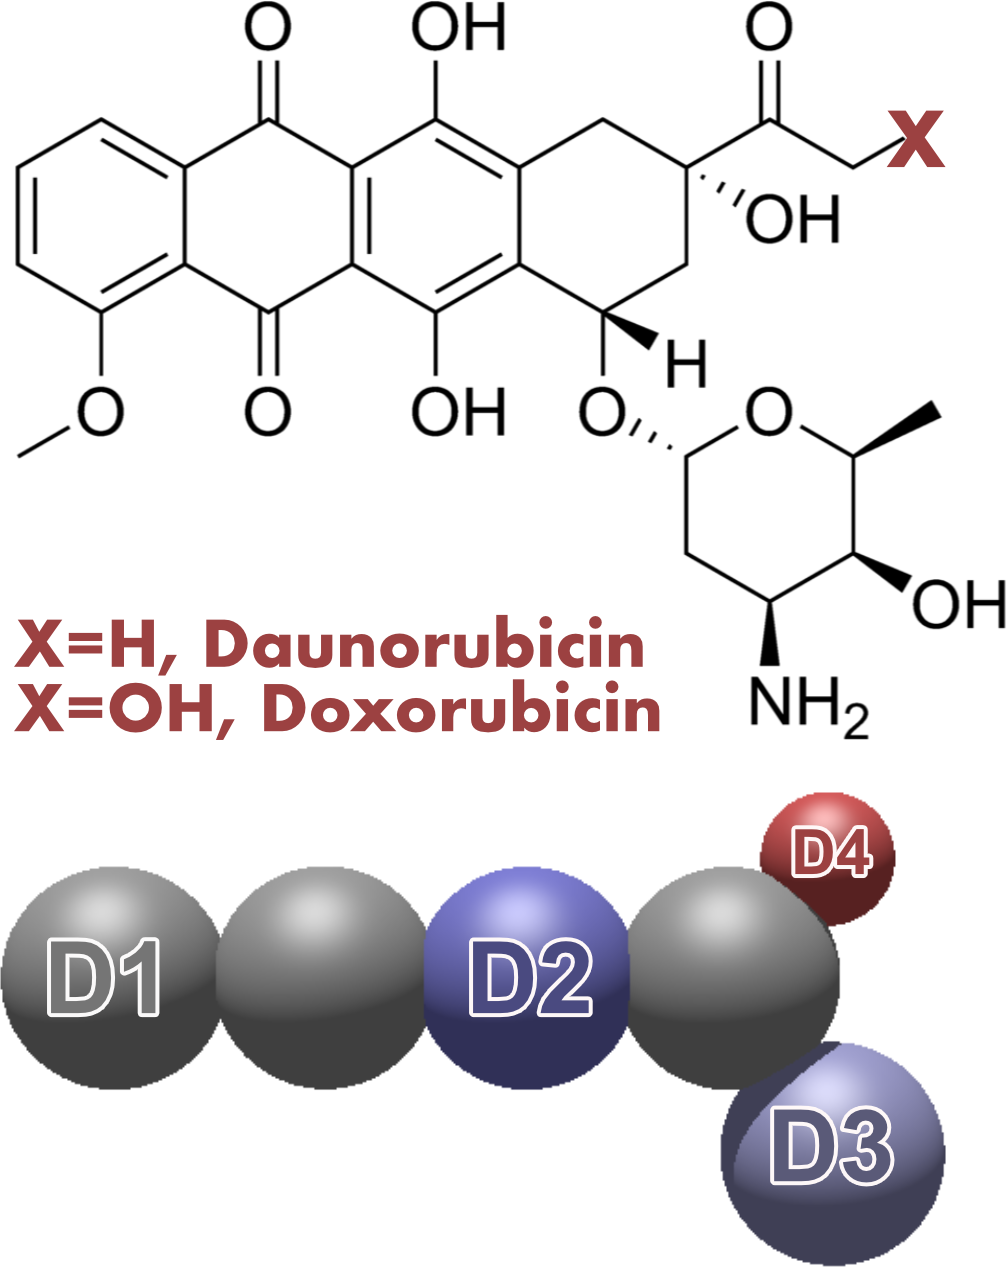
\includegraphics[width=0.35\linewidth]{Figures/graph-gel/dauno-doxo.png}
\caption{Estructura quí\'imica (arriba) y modelo de grano grueso (abajo) aplicado para describir daunorrubicina y doxorrubicina.
	Los segmentos de grano grueso $D1-D4$ se describen en la tabla \ref{table:gel:drugs}.}
\label{fig:gel:dauno-doxo}
\end{figure}


Consideraremos la absorci\'on de los f\'armacos quimioterap\'euticos Daunorrubicina (Dauno) y Doxorrubicina (Doxo) en nuestros microgeles P(NIPAm-MAA) en diferentes condiciones.
El modelo molecular aplicado para describir estos analitos se ilustra en la figura \ref{fig:gel:dauno-doxo} y la parametrizaci\'on se presenta en la tabla \ref{table:gel:drugs} \cite{PerezChavez2020}.

\begin{table}
%\small
%\begin{tabular}{lcS[table-format=-1]S[table-format=0.3]}
\centering
\begin{tabular}{|lccc|}
    \hline
    {CG unit} & {$pKa$} & {$q$ ($e$)} & {$v$ ($\text{nm}^3$)} \\
      \hline
$D1$ & - & 0 & 0.085\\
$D2$ & 7.34 & -1$^\ast$ & 0.085\\
$D3$ & 9.46 & +1$^\ast$ & 0.085\\ 
$D4$ (Doxo) & 8.46 & -1$^\ast$ & 0.035\\
$D4$ (Dauno) & - & 0 & 0.035 \\
    \hline
  \end{tabular}
 \caption{Porpediades moleculares para las distintas unidades de grano grueso usadas para el modelado de las drogas Daunorubicina y Doxorubicina. (ver figura \ref{fig:gel:dauno-doxo}).
\footnotesize ($^\ast$ Para unidades ionizables.)}
\label{table:gel:drugs} 
\end{table}




\section{Resultados y discusi\'on}
%%%%%%%%%%%%%%%%%%%%%%%%%%%%%%%%%%%%%%%%%%%%%%%%%%%%%%%%%%%%%%%%%%%%%



%%%%%%%%%%%%%%%%%%%%%%%%%%%%%%%%%%%%%%%%%%%%%%%%%%%%%%%%%%%%%%%%%%%%%
\subsection{Respuesta al pH y la concentraci\'on de sal}\label{sec:gel:pH_salt}
%%%%%%%%%%%%%%%%%%%%%%%%%%%%%%%%%%%%%%%%%%%%%%%%%%%%%%%%%%%%%%%%%%%%%


\begin{figure}[!ht]
\centering
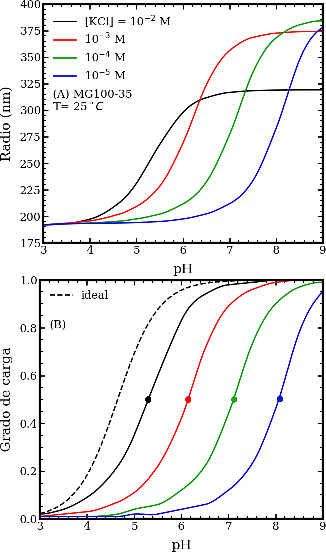
\includegraphics[width=0.5\linewidth]{Figures/graph-gel/R-pH.pdf}
\caption{Gr\'afico de tama\~no de microgel (A) y grado de carga (B) en funci\'on del pH para soluciones que tienen diferentes concentraciones de sal y $T=25 ^\circ C$.
	Las cadenas de pol\'imero en el microgel MG100-35 son $n_{ch}=100$-long. y tienen $35\% $ MAA.
	La curva de  punteada en el panel B es la disociaci\'on ideal del \'acido metacr\'ilico ($pKa=4.65$).
	Los c\'irculos de color en las curvas del panel A marcan el pKa aparente del microgel.}
\label{fig:gel:R-pH}
\end{figure}

En esta secci\'on, describiremos el comportamiento de los microgeles en respuesta a cambios en la composici\'on de la soluci\'on. Nos enfocaremos en temperaturas por debajo de la temperatura cr\'itica del PNIPAm, donde el gel experimenta un colapso. El efecto de la temperatura se evaluar\'a en la secci\'on \ref{sec:gel:temperature}.

La Figura \ref{fig:gel:R-pH}A muestra el tama\~no del microgel (radio, $R$) en funci\'on del pH para diferentes concentraciones de sal. Los microgeles de P(NIPAm-MAA) se hinchan al aumentar el pH. A medida que el pH se incrementa, un n\'umero creciente de unidades  de $MAA$ se desprotona y, por lo tanto, se cargan el\'ectricamente. La Figura \ref{fig:gel:R-pH}B muestra c\'omo la fracci\'on de $MAA$ cargados ($f$: grado de carga; ver ec. \ref{eq:gel:fcharge}) depende del pH de la soluci\'on. El hinchamiento observado en el panel A, que surge al aumentar el pH, es una respuesta a las crecientes repulsiones dentro del microgel, resultado del aumento de la carga el\'ectrica en la red polim\'erica, como se observa en el panel B.

El inicio de la transici\'on de este hinchamiento se desplaza a valores de pH m'as altos cuando se reduce la concentraci\'on de sal (ver Figura \ref{fig:gel:R-pH}A). Las curvas de disociaci\'on de protones del panel B presentan el mismo desplazamiento a pH m\'as altos, en comparaci\'on con el comportamiento ideal de un mon\'omero de $MAA$ aislado en soluci\'on diluida. Hemos discutido este comportamiento en el cap\'itulo \ref{Chapter-film}, en la secci\'on \ref{sec:film:respuesta-pH}.

El pKa aparente es el pH en el cual la mitad de los segmentos de $MAA$ se desprotonan, y este valor cuantifica el comportamiento de carga del microgel (ver Figura \ref{fig:gel:R-pH}B), as\'i como la transici\'on de expansi\'on (como se observa en el panel A, marcado con c\'irculos en $pH=pKa$). Los pKa aparentes de la Figura \ref{fig:gel:R-pH}B se muestran en la Tabla \ref{table:gel:pKa_app}.





\begin{table}[!htb]
\centering
\small
  \begin{tabular}{|cc|}
    \hline
      [NaCl] (M)&  pKa apa. ($25 ^\circ C$)  \\
      \hline
    $10^{-5}$ & 8.10  \\
    $10^{-4}$ & 7.15 \\
    $10^{-3}$ & 6.15 \\
    $10^{-2}$ & 5.35 \\
    %\azul $10^{-1}$ & \azul 4.80 \\
    ideal (pKa) &  $4.65$  \\
    \hline
  \end{tabular}
 \caption{ pka's aparente de la fig. \ref{fig:gel:R-pH} para un gel MG100-35 a $25 ^\circ C$.}
\label{table:gel:pKa_app} 
\end{table}


Una concentraci\'on relativamente alta de iones de sal dentro del microgel da como resultado el apantallamiento de las repulsiones electrost\'aticas entre los segmentos $MAA$ cargados; estas interacciones repulsivas se vuelven de corto alcance.
Cuando el pH de la soluci\'on aumenta, la disociaci\'on de los segmentos de $MAA$ sucede sin un alto costo energ\'etico originado por las repulsiones electrost\'aticas.
En estas condiciones, la desprotonaci\'on de $MAA$, inducida por la energ\'ia qu\'imica libre (equilibrio \'acido-base), se aproxima al comportamiento ideal o de una soluci\'on diluida (compar\'andose los casos de alta concentraci\'on salina con la curva de l\'inea punteada en la Figura \ref{fig:gel:R-pH}B).

Por el contrario, a bajas concentraciones de sal, el efecto de apantallamiento se debilita y las repulsiones electrost\'aticas dentro de la red son de mayor alcance.
Incluso si hay pocas cargas y distantes en la red, interactuar\'an entre s\'i.
Para reducir la contribuci\'on energ\'etica de tales repulsiones electrost\'aticas hay una disminuci\'on significativa a que las unidades $MAA$ se carguen en condiciones de baja salinidad;
en consecuencia, el pKa aparente aumenta.
El precio a pagar es aumentar la energ\'ia qu\'imica libre, cuya contribuci\'on se minimiza cuando el grado de protonaci\'on es ideal.




\begin{figure*}[!htb]
	\centering
	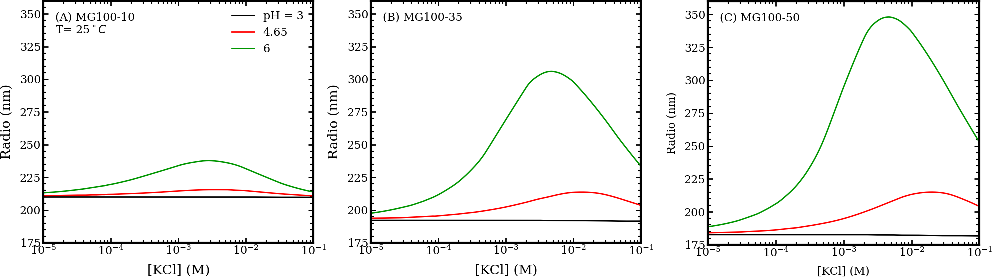
\includegraphics[width=1\linewidth]{Figures/graph-gel/R-cs.pdf}
	\caption{Gr\'afico del tama\~no del microgel en funci\'on de las concentraciones de sal para diferentes soluciones de pH y $T=25 ^\circ C$.
		Los paneles corresponden a microgeles MG-100 (longitud de cadena, $n_{ch}=100$) que tienen fracciones MAA: $10\%$ (A), $35\%$ (B) y $50\%$ (C).}
	\label{fig:gel:R-cs}
\end{figure*}


La Figura \ref{fig:gel:R-cs} ilustra c\'omo el tama\~no de los microgeles de P(NIPAm-MAA) depende de la concentraci\'on de sal para diferentes valores de pH.
A una salinidad relativamente alta, estos microgeles se hinchan con el aumento de la concentraci\'on de sal, lo que es consistente con los resultados de dispersi\'on de luz din\'amica (DLS) reportados por \citet{Wong2009} para microgeles P(NIPAm-MAA) y concentraciones de KCl en el rango de $0.1-0.5\,M$.

Las curvas de la Figura \ref{fig:gel:R-cs} muestran un comportamiento reentrante, en el que el tama\~no primero aumenta y luego disminuye al aumentar la concentraci\'on de sal.
Esta respuesta no monot\'onica es m\'as acentuada cuando la carga del pol\'imero aumenta debido a un mayor contenido de unidades de $MAA$ (observado en los diferentes paneles de la Figura \ref{fig:gel:R-cs}).

Se han informado transiciones de hinchamiento-deshinchamiento con concentraciones de sal variables en una variedad de sistemas polim\'ericos reguladores de carga.
El grosor de las capas de poli\'acidos d\'ebiles anclados es una funci\'on no monot\'onica de la concentraci\'on de sal de la soluci\'on seg\'un lo predicho por la teor\'ia del campo medio autoconsistente \cite{Israels1994, Lyatskaya1995, Zhulina1995, Gong2007}, lo cual ha sido confirmado por resultados experimentales \cite{Wu2007}.
De manera similar, los resultados te\'oricos predicen que el tama\~no de los polielectrolitos d\'ebiles ramificados en forma de estrella muestra un m\'aximo en funci\'on de la concentraci\'on de sal en la soluci\'on \cite{Borisov1998, KleinWolterink2002}.
Tambi\'en se ha predicho que el espesor de las pel\'iculas de poli\'acidos d\'ebiles entrecruzados mostrar\'a este comportamiento de hinchamiento reentrante \cite{Longo2014JCP}.






En este mismo sentido, se ha predicho una transici\'n de deshinchaci\'on a hinflaci\'on impulsada por la concentraci\'on de sal para los nanogeles de polielectrolitos fuertes \cite{jha2012understanding}. Este comportamiento, en el caso de los polielectrolitos ``quencheados", se atribuye a los efectos de volumen excluidos de los iones absorbidos a altas concentraciones salinas.

M\'as relevante para nuestro estudio, son los resultados te\'oricos de una transici\'on reentrante de hinchaci\'on a colapso para microgeles sensibles al pH y al calor \cite{polotsky2013collapse}. \citet{polotsky2013collapse} explica que el aumento de la concentraci\'on de sal promueve inicialmente la disociaci\'on de carga de los grupos \'acidos d\'ebiles hasta alcanzar la saturaci\'on, momento en el cual el grado de disociaci\'on alcanza el valor ideal. M\'as all\'a de este punto, el aumento de la concentraci\'on de sal en la soluci\'on solo mejora el apantallamiento de las repulsiones electrost\'aticas y, por lo tanto, el microgel se deshincha.

Experimentalmente, \citet{CaprilesGonzalez2008} informaron sobre el hinchamiento no monot\'onico de los microgeles de poli(NIPAm-\emph{co}-AA) (P(NIPAm-AA)) en funci\'on de la concentraci\'on de NaCl utilizando t\'ecnicas de DLS.




\begin{figure}[!tb]
	\centering
	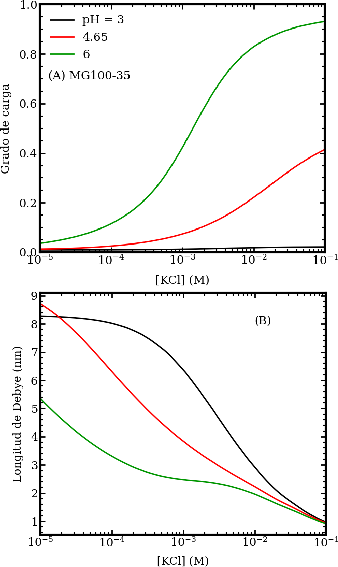
\includegraphics[width=0.5\linewidth]{Figures/graph-gel/f-cs.pdf}
	\caption{Curvas del grado de carga MAA (A) y la longitud de Debye (B) dentro de los microgeles MG100-35 en funci\'on de la concentraci\'on de sal para diferentes valores de pH.
		Estos resultados corresponden a las condiciones de figura \ref{fig:gel:R-cs}B.}
	\label{fig:gel:f-cs}
\end{figure}

El aumento de la concentraci\'on de sal de la soluci\'on tiene dos efectos opuestos sobre las propiedades del microgel. Por un lado, aumenta el apantallamiento de interacciones de carga a medida que se cargan los iones dentro del gel; las repulsiones electrost\'aticas entre los mon\'omeros de $MAA$ cargados est\'an cada vez m\'as protegidas. El alcance efectivo de estas repulsiones se acorta, favoreciendo el deshinchamiento. Por otro lado, este apantallamiento permite una mayor desprotonaci\'on de los mon\'omeros de $MAA$, promovida por el equilibrio \'acido-base. La disociaci\'on de carga favorece el hinchamiento para reducir las repulsiones electrost\'aticas.

La figura \ref{fig:gel:f-cs} ilustra este doble efecto de aumentar la concentraci\'on de sal en la soluci\'on, lo que conduce al comportamiento de hinchamiento-deshinchamiento. El panel A muestra que la carga del microgel aumenta mon\'otonamente con la concentraci\'on de sal. En el panel B, usamos la longitud de Debye para cuantificar la extensi\'on de las interacciones electrost\'aticas.% (consulte la ecuaci'on \ref{eq:debye_length} en el suplemento). 
El alcance efectivo de estas interacciones se acorta dentro del microgel a medida que aumenta la concentraci\'on de sal. Se puede observar en la figura \ref{fig:gel:f-cs} que en condiciones de pH 3 la carga dentro del microgel es insignificante, lo que resulta en un hinchamiento muy poco apreciable en la figura \ref{fig:gel:R-cs}B.

Esta teor\'ia requiere que el interior del microgel sea de carga neutra. La congujaci\'on de cargas y contraiones debe estar equilibrada. \citet{Claudio2009} demostr\'o que esta es una aproximaci\'on razonable cuando el microgel es m\'as grande que $R = 125,\text{nm}$ y tiene un 50\% de mon\'omeros cargados. Los microgeles P(NIPAm-MAA) aqu\'i planteados son m\'as grandes que ese tama\~no en la mayor\'ia de las condiciones, particularmente cuando el pH est\'a por encima del pKa aparente y la mayor\'ia de los grupos $MAA$ est\'an desprotonados. Adem\'as, los iones de sal se absorben dentro del microgel para reforzar dicha restricci\'on, lo que permite que los segmentos de $MAA$ se desprotonen y se carguen el\'ectricamente. Describimos este efecto como el apantallamiento de las repulsiones electrost\'aticas entre los grupos de $MAA$, que es un concepto que hemos discutido con anterioridad.


\subsection{Respuesta a la Temperatura}\label{sec:gel:temperature}
%%%%%%%%%%%%%%%%%%%%%%%%%%%%%%%%%%%%%%%%%%%%%%%%%%%%%%%%%%%%%%%%%%%%%

\begin{figure*}[!htb]
	\centering
	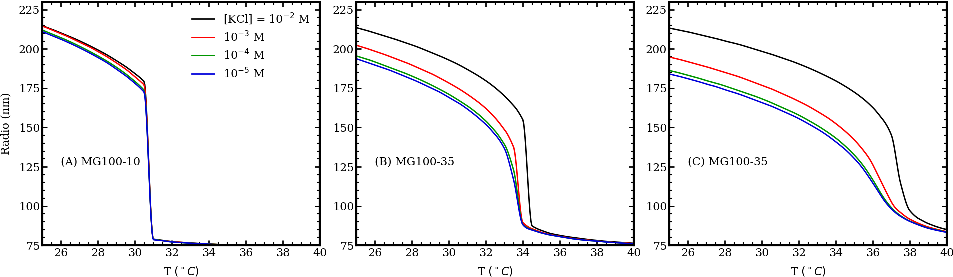
\includegraphics[width=1\linewidth]{Figures/graph-gel/R-T.pdf}
	\caption{Gr\'afico del tama\~no del microgel en funci\'on de la temperatura para diferentes concentraciones de sal en soluci\'on y $pH~4,65$.
		Los paneles corresponden a microgeles MG-100 (longitud de cadena, $n_{ch}=100$) que tienen diferentes fracciones de $MAA$: $10\%$ (A), $35\%$ (B) y $50\%$ (C).}
	\label{fig:gel:R-T}
\end{figure*}

Discutido el efecto del pH y la concentraci\'on de sal, ahora nos enfocaremos en mostrar la respuesta de los microgeles de P(NIPAm-MAA) frente a cambios en la temperatura.
En cada panel de la figura \ref{fig:gel:R-T} se muestra el tama\~no de tres geles MG-100 como funci\'on de la temperatura a distintas concentraciones salinas.
A baja temperatura, estos microgeles muestran un estado relativamente hinchado, mientras que a altas temperaturas se produce un estado colapsado (alta densidad de pol\'imero).

Esto \'ultimo ocurre dado que el NIPAm adquiere un comportamiento hidrof\'obico por encima de su temperatura de transici\'on cr\'itica inferior (LCST por sus siglas en ingl\'es), expulsando el solvente de su interior y colapsando su estructura \cite{sbeih2019structural}.
El tama\~no del gel en este estado es robustamente independiente de la concentraci\'on salina o el pH y posee un radio muy cercano al del microgel seco (ver tabla \ref{table:gel:optimal-R}).

Por otro lado, el estado hinchado del gel est\'a dominado por las repulsiones electrost\'aticas entre los segmentos de $MAA$ cargados y los contraiones absorbidos, como fue descrito en la secci\'on \ref{sec:gel:pH_salt}.
El tama\~no y la carga del microgel son funciones mon\'otonamente decrecientes de la temperatura.
El estado hinchado se caracteriza por un mayor grado de carga.
De hecho, la transici\'on de volumen, de estados hinchado a colapsado, est\'a acompa\~nada por una transici\'on en el grado de carga de los segmentos de $MAA$.


\textcolor{red}{OJO QUE FALTARIA REFERIR A UNA FIGURA}

\begin{figure}[!htb]
	\centering
	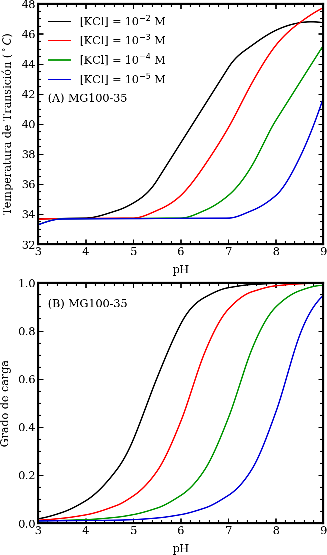
\includegraphics[width=0.5\linewidth]{Figures/graph-gel/Tpt-pH.pdf}
	\caption{Gr\'aficos que muestran la temperatura de transici\'on de volumen $T_{TV}$ (A) y la fracci\'on de $MAA$ cargado a esta temperatura (B) en funci\'on del pH para diferentes concentraciones de sal.
		Este microgel P(NIPAm-MAA) tiene una longitud de cadena de $n_{ch}=100$ y un MAA de $35\%$.}
	\label{fig:gel:Tpt-pH}
\end{figure}


En la mayor\'ia de las condiciones, pero no en todas, la transici\'on entre estos dos estados del microgel es brusca y ocurre en un rango estrecho alrededor de una temperatura bien definida, que definimos como Temperatura de Transici\'on de Volumen ($T_{TV}$). Comparando los diferentes paneles de la figura \ref{fig:gel:R-T}, vemos que aumentar el contenido de $MAA$ de los microgeles conduce a una transici\'on m\'as suave alrededor de $T_{TV}$.

La figura \ref{fig:gel:Tpt-pH}A muestra que la $T_{TV}$ aumenta con el pH y la concentraci\'on de sal. Estos resultados son consistentes con los experimentos de DLS que muestran que la temperatura de transici\'on volum\'etrica de los microgeles P(NIPAm-MAA) aumenta con el pH \cite{Kleinen2008}, lo que tambi\'en se ha observado para los microgeles P(NIPAm-AA) \cite{CaprilesGonzalez2008}. Se ha definido $T_{TV}$ como el punto de inflexi\'on de las curvas $R(T)$ de la figura \ref{fig:gel:R-T} entre los estados hinchado y colapsado \cite{Kratz2001}.

El panel B de la figura \ref{fig:gel:Tpt-pH} muestra el grado de carga de los segmentos de $MAA$ en el $T_{TV}$. Existe una clara correlaci\'on entre la dependencia de $T_{TV}$ con el pH y la salinidad, y el estado de carga del microgel en las condiciones VPT. La temperatura de transici\'on aumenta con el pH y la concentraci\'on de sal, al igual que la carga de la red de pol\'imeros.

A diferencia de este comportamiento, el VPTT de los microgeles basados en PNIPAm permanentemente cargados disminuye con la concentraci\'on de sal \cite{Lopez2020}. En este caso, la carga del pol\'imero permanece constante, mientras que la incorporaci\'on de iones de sal solo debilita las repulsiones electrost\'aticas entre las cargas.

\begin{figure}[!tb]
	\centering
	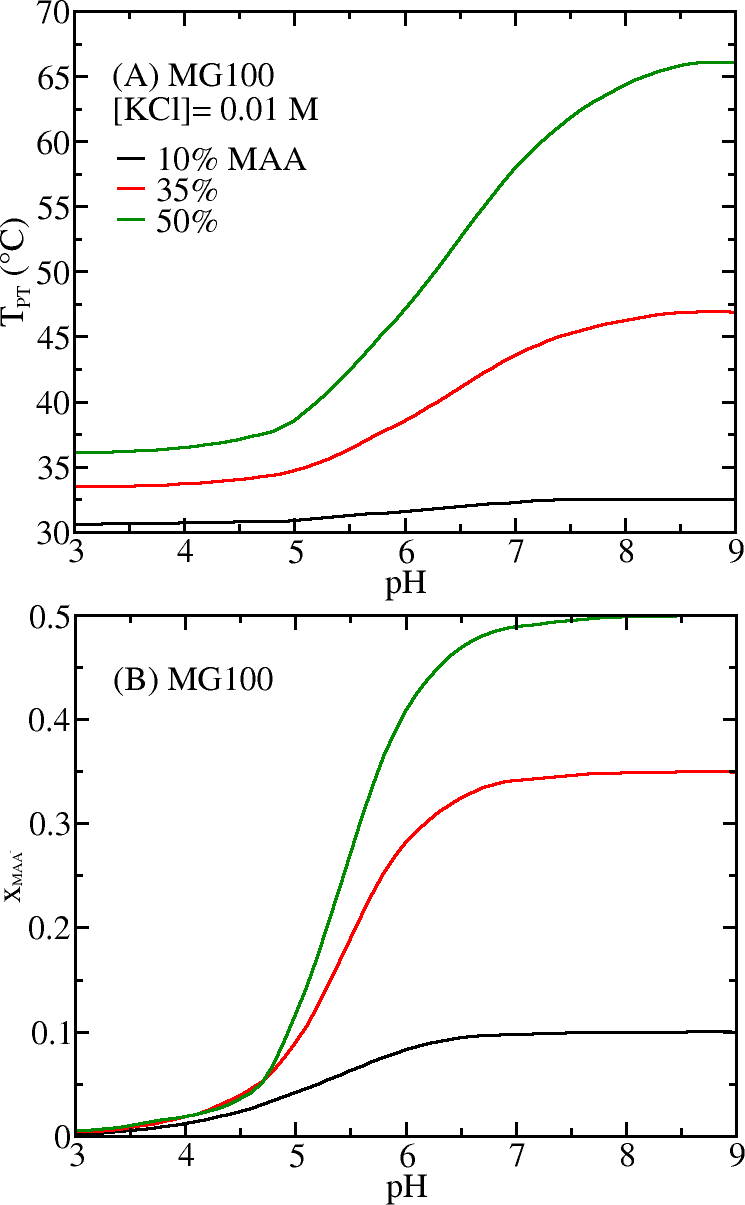
\includegraphics[width=0.5\linewidth]{Figures/graph-gel/Tpt-pH_MAA.png}
	\caption{(A) Gr\'afico de temperatura de transici\'on $T_{TV}$ en funci\'on del pH para microgeles MG-100 (longitud de cadena de pol\'imero, $n_{ch}=100$ segmentos) que tienen diferentes contenidos de MAA; $[KCl]=0.01 M$;
	(B) Fracci\'on de segmentos cargados $x_{MAA^-}=\frac{N_{MAA^-}}{N_{seg}}$ en funci\'on del pH para las mismas condiciones del panel A (\emph{i.e.} , en el $T_{TV}$); $x_{MAA^-}$ es proporcional a la carga total del pol\'imero; $N_{seg}$ es el mismo para todos los microgeles.}
	\label{fig:gel:Tpt_MAA}
\end{figure}

Los resultados de la figura \ref{fig:gel:Tpt-pH} muestran que la temperatura de transici\'on est\'a controlada por la cantidad de carga dentro del microgel. De hecho, aumentar el contenido de MAA tiene el mismo efecto de desplazar el VPTT a valores m\'as altos, como se observa en la figura \ref{fig:gel:Tpt_MAA}A. Una vez m\'as, este comportamiento resulta de una estructura polim\'erica m\'as cargada.

Para comparar el estado de carga de microgeles con diferentes contenidos de $MAA$, utilizamos la fracci\'on total de mon\'omeros cargados:

\begin{equation}
	x_{MAA^-}=\frac{N_{MAA^-}}{N_{seg}}=f x_{MAA}
\end{equation}

Donde $N_{MAA^-}$ es el n\'umero de segmentos MAA desprotonados, todas las dem\'as cantidades se han definido en la secci\'on \ref{sec:gel:theory}. $x_{MAA^-}$ es proporcional a la carga total de la red de microgel, y debido a que todos los microgeles tienen el mismo n\'umero total de segmentos, la constante proporcional es la misma para todos los contenidos de $MAA$ considerados. La figura \ref{fig:gel:Tpt_MAA}B muestra que existe una clara correlación entre $T_{TV}$ y la carga total del microgel (dada por $x_{MAA^-}$) al cambiar el pH o el contenido de $MAA$ del pol\'imero.


%%%%%%%%%%%%%%%%%%%%%%%%%%%%%%%%%%%%%%%%%%%%%%%%%%%%%%%%%%%%%%%%%%%%%
\subsection{Efecto del grado de entrecruzamiento} \label{sec:gel:entrecruzamiento}
%%%%%%%%%%%%%%%%%%%%%%%%%%%%%%%%%%%%%%%%%%%%%%%%%%%%%%%%%%%%%%%%%%%%%


\begin{figure*}[!tb]
	\centering
	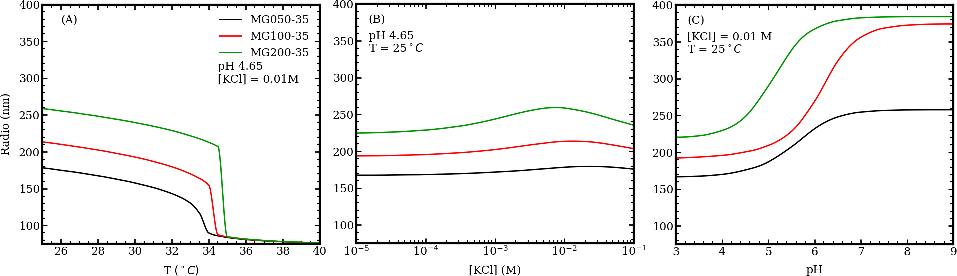
\includegraphics[width=1\linewidth]{Figures/graph-gel/R-all_xlink.pdf}
	\caption{Gr\'afico del tama\~no del microgel en funci\'on de la temperatura, la concentraci\'on de sal y el pH (paneles A, B y C respectivamente).
		Diferentes curvas corresponden a microgeles con segmentos de $50$ (MG050), $100$ (MG100) y $200$ (MG200) por cadena de pol\'imero, todos con $35\%$ MAA.}
	\label{fig:gel:R_xlink}
\end{figure*}

En esta instancia vamos a analizar c\'omo el grado de entrecruzamiento de la red polim\'erica afecta el comportamiento previamente descrito de nuestro gel. Consideramos microgeles con segmentos de $50$, $100$ y $200$ por cadena, manteniendo el mismo n\'umero total de segmentos. A medida que la cantidad de segmentos por cadena disminuye, aumenta el grado de entrecruzamiento en el microgel. La figura \ref{fig:gel:R_xlink} muestra la respuesta de los microgeles con un porcentaje de $MAA$ del $35\%$ ante cambios de temperatura (panel A), concentraci\'on de sal (panel B) y pH (panel C).

Los microgeles con menor grado de entrecruzamiento (mayor n\'umero de segmentos por cadena) presentan un mayor grado de hinchamiento. Este comportamiento de los microgeles P(NIPAm-MAA) ha sido confirmado experimentalmente \cite{khan2013preparation}. Cualitativamente, la respuesta a la concentraci\'on de sal y al pH es similar para todas las longitudes de cadena consideradas (paneles B y C de la figura \ref{fig:gel:R_xlink}, respectivamente). Una observaci\'on interesante es que la disminuci\'on del grado de entrecruzamiento conduce a una transici\'on de volumen m\'as brusca a medida que aumenta la temperatura (figura \ref{fig:gel:R_xlink}A), y adem\'as, la temperatura de transici\'on de volumen ($T_{TV}$) aumenta. Estos resultados son consistentes con los trabajos de \citet{li1989study} y \citet{wu1997volume}, quienes informaron un cambio en la transici\'on de volumen de NIPAm de continua a discontinua a medida que disminuye la concentraci\'on del entrecruzante en la s\'intesis.

En la figura \ref{fig:gel:R_xlink}, tambi\'en se observa que el aumento de la longitud de la cadena (disminuci\'on del grado de entrecruzamiento) desplaza la temperatura de transici\'on de volumen ($T_{TV}$) hacia valores m\'as altos. Esto concuerda con los resultados de la espectroscopía UV realizada por \citet{Lee2008} para los microgeles P(NIPAm-AA). Este comportamiento se observa en todo el rango de condiciones exploradas en este cap\'itulo.

La constante de fuerza de la contribuci\'on el\'astica a la energ\'ia libre es inversamente proporcional a la longitud de la cadena $n_{ch}$ (ver ecuaci\'on \ref{eq:gel:free-energy}). Al reducir el grado de entrecruzamiento, el microgel se hincha y se vuelve m\'as flexible, lo que permite una mayor carga en la red de pol\'imero. En consecuencia, se requiere una temperatura m\'as alta para inducir el colapso de la red de pol\'imero. Hemos demostrado que la temperatura de transici\'on de volumen ($T_{TV}$) est\'a fuertemente correlacionada con el grado de carga.

La presencia de unidades \'acidas acent\'uaa la dependencia de la $T_{TV}$ con la longitud de la cadena, ya que incorpora el equilibrio de protonaci\'on al balance energ\'etico. Sin embargo, este comportamiento es intr\'inseco a la interacci\'on entre las propiedades hidrof\'obicas y la elasticidad de la red polim\'erica. De hecho, la temperatura de transici\'on de los microgeles de PNIPAm puros tambi\'en aumenta con la longitud de la cadena, aunque el efecto es significativamente m\'as d\'ebil en ausencia de segmentos de $MAA$.



%%%%%%%%%%%%%%%%%%%%%%%%%%%%%%%%%%%%%%%%%%%%%%%%%%%%%%%%%%%%%%%%%%%%%
\subsection{Adsorci\'on de drogas}\label{sec:gel:ads-drogas}
%%%%%%%%%%%%%%%%%%%%%%%%%%%%%%%%%%%%%%%%%%%%%%%%%%%%%%%%%%%%%%%%%%%%%


Los microgeles polim\'ericos se han destacado como transportadores inteligentes de medicamentos debido a sus propiedades \'unicas. Estos sistemas nanoestructurados (en este caso microestrucutrados) ofrecen una plataforma vers\'atil para la encapsulaci\'on, protecci\'on y liberaci\'on controlada de sustancias bioactivas. Los microgeles pueden responder a est\'imulos externos,como hemos mostrados en las secciones anteriores,  como cambios de pH, temperatura y concentraci\'on de iones, lo que les permite liberar su carga terap\'eutica de manera selectiva y espec\'ifica en el sitio deseado. 

Por ejemplo, se sabe que el pH extracelular del tejido tumoral es m\'as bajo que el del tejido sano \cite{Gerweck1996}, lo que hace que los microgeles respondan al pH sean idoneos para la administraci\'on local de medicamentos contra el c\'ancer \cite{Dadsetan2013}.

Peppas \emph{et al.} han estudiado ampliamente los microgeles sensibles al pH basados en $MAA$ como transportadores inteligentes que pueden operar utilizando los diferentes niveles de acidez a lo largo del tracto digestivo y prevenir la degradaci\'on de f\'armacos en el est\'omago \cite{TorresLugo2002, Carr2010, DuranLobato2014, Sharpe2018}.

En esta secci\'on, evaluamos la capacidad de los microgeles P(NIPAm-MAA) para incorporar dos f\'armacos quimioterap\'euticos. En particular, investigamos las mejores condiciones para la encapsulaci\'on de f\'armacos en condiciones de laboratorio. Consideramos que la doxorrubicina (Doxo) y la daunorrubicina (Dauno) son dos de las antraciclinas importantes y ampliamente utilizadas en la quimioterapia para tratar una amplia gama de c\'anceres \cite{Panis2012, Carvalho2009, aubel1984daunorubicin,come1999dual}. Estas drogas se pueden seguir utilizando fluorescencia y adsorbancia, lo que las hace atractivas desde el punto de vista de la investigaci\'on \cite{Serpe2005, ThanHtun2009, PerezChavez2020}. Adem\'as, estos f\'armacos pueden adquirir carga positiva en la mayor\'ia de las condiciones, lo que puede facilitar su encapsulaci\'on en microgeles de pol\'imeros ani\'onicos \cite{Li2019}. \citet{Serpe2005} han estudiado la captaci\'on y liberaci\'on termicamente activadas de Doxo a partir de pel\'iculas capa por capa de microgeles de P(NIPAm-AA) y poli(clorhidrato de alilamina). M\'as recientemente, utilizando resonancia magn\'etica nuclear de lapso de tiempo, \citet{MartinezMoro2020} han descrito la interacci\'on entre Doxo y microgeles P(NIPAm-MAA) en diferentes condiciones.
\begin{figure}[!tb]
	\centering
	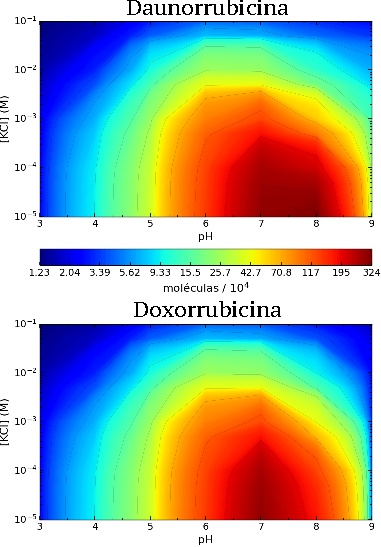
\includegraphics[width=0.55\linewidth]{Figures/graph-gel/drug_ads.pdf}
	\caption{Mapas en color que muestran el n\'umero de mol\'eculas de daunorrubicina (A) y doxorrubicina (B) absorbidas por microgel en funci\'on del pH de la soluci\'on y la concentraci\'on de sal.
		La concentraci\'on de f\'armaco en soluci\'on es $1mM$ y $T=25 ^\circ C$.
		el microgel P(NIPAm-MAA) tiene $n_{ch}=100$ de longitud de cadena y $35\%$ MAA (MG100-35).}
	\label{fig:gel:drug_ads}
\end{figure}


La figura \ref{fig:gel:drug_ads} ilustra el n\'umero de mol\'eculas de Dauno (panel A) y Doxo (panel B) dentro del microgel en relaci\'on con la concentraci\'on de sal y el pH de la soluci\'on. Se observa que las condiciones \'optimas para la encapsulaci\'on de estos f\'armacos terap\'euticos corresponden a una baja concentraci\'on de sal y un pH de 6 a 8. La reducci\'on en la concentraci\'on de sal favorece la absorci\'on. Tanto Dauno como Doxo presentan una carga neta de $+1$ a pH \'acido y neutro (ver la figura \ref{fig:gel:carga-drug_ads}).

\begin{figure}[!tb]
	\centering
	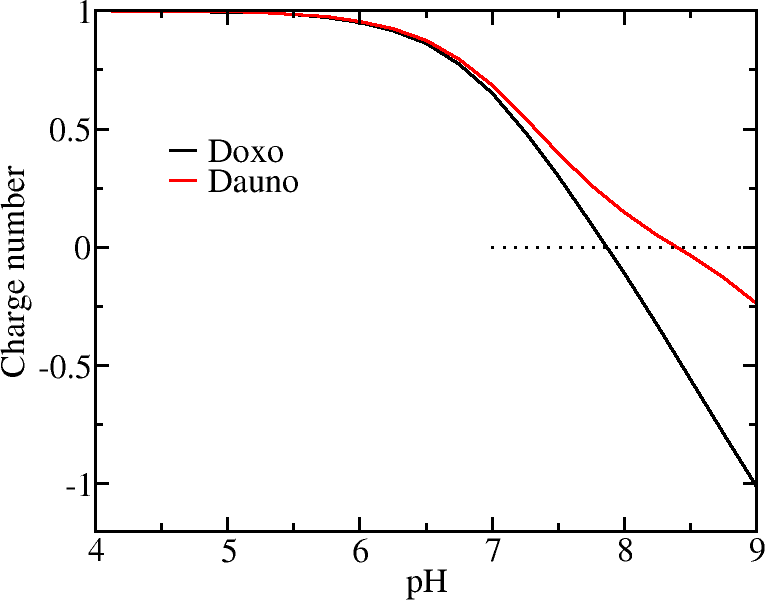
\includegraphics[width=0.9\linewidth]{Figures/graph-gel/drugs-Q.png}
	\caption{N\'umero de carga de las drogas estudiadas: Doxo y Dauno. La intersecci\'on con la l\'inea a puntos muestra el punto isolectrico de las mismas. Pasado este punto se da una inversi\'on en la carga de las drogas lo que conlleva a una respulsi\'on electrost\'atica con los segmentos cargados de $MAA$ del microgel. }
	\label{fig:gel:carga-drug_ads}
\end{figure}

Como resultado, la absorci\'on de Dauno y Doxo tiene que competir con la absorci\'on de iones de potasio para neutralizar la carga negativa de la red del pol\'imero (\citet{PerezChavez2020}). En la figura \ref{fig:gel:f-cs}, se observa que en ausencia de un f\'armaco disuelto, la carga del microgel disminuye a medida que se reduce la concentraci\'on de sal, lo que aparentemente entra en conflicto con la mejora de la absorci\'on observada en la figura \ref{fig:gel:drug_ads} bajo estas condiciones. Sin embargo, despu\'es de la absorci\'on del f\'armaco, el grado de carga de los segmentos de MAA aumenta significativamente, especialmente en condiciones de baja concentraci\'on de sal. Adem\'as, es importante destacar que este comportamiento est\'a particularmente asociado con la relativamente alta concentraci\'on de f\'armaco considerada en estos resultados ($1\, mM$).

La fracci\'on de segmentos de $MAA$ cargados negativamente en el pol\'imero aumenta con el pH, lo que explica por qu\'e tambi\'en aumenta la absorci\'on de Dauno/Doxo en condiciones \'acidas. Sin embargo, en condiciones alcalinas, la carga neta positiva de estos f\'armacos disminuye con el aumento del pH, lo que desfavorece su absorci\'on. Por lo tanto, la absorci\'on de Dauno/Doxo es una funci\'on no mon\'otona del pH.

En nuestro modelo, los puntos isoel\'ectricos de Dauno y Doxo son 8.4 y 7.9, respectivamente ver fig. \ref{fig:gel:carga-drug_ads}. La figura \ref{fig:gel:drug_ads} muestra que la adsorci\'on de ambas mol\'eculas puede ser significativa alrededor y por encima de estos valores de pH. En otras palabras, hay una adsorci\'on considerable de mol\'eculas con carga negativa dentro de la red de nuestro gel con carga similar. Aunque estas mol\'eculas est\'an cargadas negativamente en la fase de soluci\'on, la absorci\'on ocurre porque el pH disminuye dentro del microgel, lo que permite que los f\'armacos regulen su carga el\'ectrica y permanezcan cargados positivamente dentro del microgel (fig. \ref{fig:gel:drug_pH}).


\begin{figure}[!tb]
	\centering
	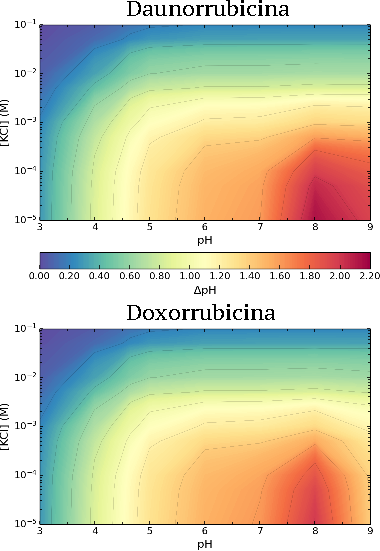
\includegraphics[width=0.55\linewidth]{Figures/graph-gel/drug_pH.pdf}
	\caption{Mapas en color que muestran el cambio en el pH dentro del microgel, $\Delta pH = pH - pH_{GEL}$ en funci\'on de sal y el pH de la soluci\'on para daunorrubicina (A) y doxorrubicina (B). Estos cambios son reportados para las mismas condiciones de \ref{fig:gel:drug_ads}, es decir:
		La concentraci\'on de f\'armaco en soluci\'on es $1mM$ y $T=25 ^\circ C$.
		el microgel P(NIPAm-MAA) tiene $n_{ch}=100$ de longitud de cadena y $35\%$ MAA (MG100-35).}
	\label{fig:gel:drug_pH}
\end{figure}

El punto isoel\'ectrico m\'as bajo de la doxorrubicina se debe a la desprotonaci\'on de su grupo hidroxilo sustituyente (v\'ease  el segmento $D4$ en la figura \ref{fig:gel:dauno-doxo} y tabla \ref{table:gel:drugs}). Como resultado de esta carga negativa adicional en condiciones alcalinas, el rango de pH de adsorci\'on es ligeramente m\'as amplio para la daunorrubicina.

\section{Conclusiones}

En este cap\'itulo mostramos una teor\'ia termodin\'amica  para un sistema compuesto de dos fases con el cual se describe la respuesta de diferentes nano/microgeles de P(NIPAm-MAA) a los cambios en el pH, la concentraci\'on de sal y la temperatura.
Estas part\'iculas suaves se hinchan con el aumento del pH, lo cual es resultado de las repulsiones electrost\'aticas entre los segmentos cargados de MAA a medida que se disocian.
Este comportamiento de hinchamiento est\'a controlado por la carga \cite{FernandezNieves2000}.
El inicio de esta transici\'on impulsada por el pH se puede caracterizar adecuadamente utilizando el pKa aparente de los segmentos de MAA, que se desplaza a valores de pH m\'as altos a medida que disminuye la concentraci\'on de sal en la soluci\'on.

A pH constante y por debajo de la temperatura de transici\'on de fase inferior cr\'itica (LCST) del PNIPAm, el tama\~no de estos microgeles es una funci\'on no mon\'otona de la concentraci\'on de sal.
El aumento de la salinidad de la soluci\'on puede provocar tanto hinchamiento como deshinchamiento, dependiendo del rango de concentraci\'on de sal.
Esta transici\'on de hinchamiento-deshinchamiento inversa surge como resultado de la competencia entre los efectos opuestos del aumento de la concentraci\'on de sal en los sistemas de polielectrolito d\'ebil, que tanto promueve la disociaci\'on de la carga como mejora el apantallamiento de las repulsiones electrost\'aticas.


A medida que aumenta la temperatura, se produce una transici\'on de fase de volumen diferente que est\'a asociada a la hidrofobicidad intr\'inseca del PNIPAm por encima de su LCST.
La temperatura de transici\'on de fase de volumen de estos microgeles depende de la cantidad de MAA en el pol\'imero, el grado de entrecruzamiento, el pH de la soluci\'on y la concentraci\'on de sal.
Cambiar estas variables independientes y/o los par\'ametros de dise\~no son formas de modificar el estado de carga del microgel.
El mensaje principal de este cap\'itulo es que la cantidad de carga en la estructura del pol\'imero controla la temperatura de transici\'on de fase de volumen de los microgeles multiresponsivos.

Tambi\'en hemos evaluado la capacidad de estes microgeles para encapsular dos f\'armacos quimioterap\'euticos t\'ipicos con carga positiva.
El mejor enfoque para mejorar la partici\'on de estos f\'armacos en el microgel es reducir la concentraci\'on de sal en la soluci\'on.
M\'as sorprendente es el hecho de que las mejores condiciones de encapsulaci\'on corresponden a valores de pH alrededor o por encima de los puntos isoel\'ectricos de estos f\'armacos, donde estas mol'eculas tienen carga negativa en la soluci\'on de encapsulaci\'on. 
\chapter{esfericas}

%%%%%%%%%%%%%%%%%%%%%%%%%%%%%%%%%%%%%%%%%%%%%%%%%%
\section{Introduction}
%%%%%%%%%%%%%%%%%%%%%%%%%%%%%%%%%%%%%%%%%%%%%%%%%%


En estas secci\'on... geles polim\'ericos... 
Se aborda una perspectiva diferente con informaci\'on a la que no era posible acceder con el modelo anterior.
El conocimiento  de la estructura interna, o una aproximaci\'on de ella nos abre las puertas al dise\~no de m\'as y mejores materiales...

%%%%%%%%%%%%%%%%%%%%%%%%%%%%%%%%%%%%%%%%%%%%%%%%%%
\section{Method: Molecular Theory}
%%%%%%%%%%%%%%%%%%%%%%%%%%%%%%%%%%%%%%%%%%%%%%%%%%

El estudio de estos nanogeles conlleva un formalismo similar al visto en el capitulo de los films polim\'ericos y al modelo de dos fases.


Es decir buscamos con este m\'etodo  minimizar una energ\'ia libre del sistema.
Incorporaando una caracterizaci\'on molecular de grano grueso de las diversas especies qu\'imicas presentes.

El sistema en estudio es un solo nanogel en equilibrio con una solución acuosa que tiene una composici\'on de bulk definida externamente.
Es decir, el pH, la concentraci\'on de sal y la concentració'o de prote\'ina son las variables independientes.
La red polim\'erica que da estructura al nanogel contiene dos tipos de segmentos: una unidad sensible al pH, ya sea \'acida (MAA) o b\'asica (AH), y un segmento neutro (VA);
los segmentos que componene al entrecruzante en nuestra red se describen como segmentos de carga neutral.

Como vimos en... la energ\'ia libre se convierte en un gran potencial el cual nos permite un mejor manejo y resoluci]'on del sistema.
Este potencial contiene las siguientes contribuciones:

\begin{align}
\begin{aligned}
\Omega_{NG}=& -TS_{mez} -TS_{conf,net} + F_{qca,net} + F_{qca,pro}\\
& + U_{elec} + U_{ste} + U_{vdw} - \sum_{\gamma}{\mu_\gamma N_\gamma} - \mu_{pro} N_{pro}
\end{aligned}
\label{eq:esf:semicano}
\end{align}


\noindent donde $S_{mez}$ es la entrop\'ia de traslaci\'on (y de mezcla) de las especies de la soluci\'on: mol\'eculas de agua (H$_2$O), iones de hidronio (H$_3$O$^+$), iones de hidr\'oxido (OH$^- $), cationes de sal, aniones de sal y prote\'ina.
Consideramos una sal monovalente, NaCl completamente disociada en iones de sodio (Na$^+$) y cloruro (Cl$^-$).
$S_{conf,net}$ representa la entrop\'ia conformacional que resulta de la flexibilidad de la red de pol\'imeros, que puede asumir muchas conformaciones diferentes.
$F_{qca,net}$ es la energ\'ia qu\'imica libre que describe el equilibrio entre las especies protonadas y desprotonadas de unidades funcionales (\'acidas/b\'asicas) en el pol\'imero.
De manera similar, $F_{qca,pro}$ describe la protonaci\'on de residuos titulables de la prote\'ina.
$U_{elec}$ y $U_{ste}$ representan, respectivamente, las interacciones electrost\'aticas y las repulsiones est\'ericas.
$U_{Vdw}$ contiene las interacciones de Van der Waals entre los distintos segmentos y el solvente.
Finalmente, la suma de $\gamma$ expresa el equilibrio qu\'imico entre nuestro sistema y la soluci\'on bulk que representa un ``ba\~no t\'ermico" para las part\'iculas libres, donde $\mu_\gamma$ y $N_\gamma$ son el potencial qu\'imico y el n\'umero de mol\'eculas de especie $\gamma$, respectivamente;
el sub\'indice $\gamma$ recorre las especies qu\'imicas libres.
El siguiente t\'ermino tiene en cuenta el equilibrio descrito anteriormente, pero en esta ocasi\'on para la prote\'ina.

Las expresiones explicitas de cada uno de estos componentes, as\'i como la minimizaci\'on de nuestro gran potencial es descrita en la siguiente secci\'on.



\subsection{Teoria red polim\'erica}\label{sec:esf:tm}

A continuaci\'on describiremos la forma expl\'icita de cada uno de estos t\'erminos, donde los segmentos protonables del nanogel ser\'an considerados como segmentos de \'acido metacrílico (MAA). Sin embargo, las mismas ecuaciones se aplican a los nanogeles que tienen segmentos b\'asicos. Las diferencias se encuentran en el uso del signo del grado de disociaci\'on.

En primera instancia tenemos la entrop\'ia de traslaci\'on y de mezcla de las especies m\'oviles, incluida la prote\'ina:


\begin{align}
	\begin{aligned}
		-\frac{S_{mez}}{k_B}= &\sum_{\gamma}\int_0^\infty{dr G(r)\rho_\gamma(r)\left(\ln \left(\rho_\gamma (r)v_w\right) -1 + \beta\mu^0_\gamma\right)} \\
		&+ \sum_{\theta}\int_0^\infty{dr G(r)\rho_{pro}(\theta,r)\left(\ln \left(\rho_{pro}(\theta,r)\right) -1 + \beta\mu^0_{pro} \right)}
	\end{aligned}
\end{align}



\noindent donde $\beta = \frac{1}{k_BT}$, $k_B$ es la constante de Boltzmann y $T$ la temperatura absoluta del sistema, $\rho_\gamma(r)$ y $\mu_\gamma$ es la densidad local, en la posici\'on $r$, y potencial qu\'imico de la especie $\gamma$ respectivamente.
El sub\'indice $\gamma$ toma en cuenta las mol\'eculas de agua y sus iones (hidronio e hidr\'oxido), y los iones disociados de la sal ($K^+$, $Cl^-$). $G(r)$ es la constante de simetr\'ia de nuestro sistema, en particular para cada para $r$: $G(r) =4\pi r^2$. Esta \'utima se ejemplificara de mejor forma en la secci\'on del modelado molecular.

El segundo t\'ermino de la entrop\'ia de mezcla que considera los aportes entr\'opicos de la prote\'ina.
$\rho_{pro}(\theta,r)$ es la densidad local de la prote\'ina en la conformaci\'on  $\theta$.  La prot\'ina puede tomar cualquier conformaci\'on presenten en su set de conformaciones $\{\theta \}$
La contribuci\'on entr\'opica tambi\'en incluye la rotación espacial.
La densidad media local total de prote\'ina es: 


\begin{align}
	\left<\rho_{pro}(r)\right> = \sum_\theta{\rho_{pro}(\theta,r)}
\end{align}




$S_{conf,net}$ representa la entrop\'ia conformacional resultante de la flexibilidad de la red polim\'erica que forma al nanogel. Estas 
conformaciones son  denotadas por el set $\{\alpha\}$. 
\begin{equation}
	\frac{S_{conf,nw}}{k_B} = - \sum_{\alpha}{P(\alpha)\ln P(\alpha)}
\end{equation}


\noindent En donde $P(\alpha)$ muestra la probabilidad que el nanogles se encuentre un a configuraci\'on $\alpha$.
Una conformaci\'on $\alpha$ viene especificada por la posici\'on de todos sus segmentos. 
La fracci\'on en volumen de estos segmentos puede expresarse como:

%%%%%% modificacion 1
\begin{align}
	\left< \phi^i(r)\right> = \sum_\alpha{P(\alpha)\phi^i_r(\alpha,r)} 
	\label{eq:esf:ensamble-gel}
\end{align}

\noindent en donde $\frac{\phi^i_r(\alpha,r)}{v_i}$ define la densidad de segmentos entre las esferas de radio $\textbf{r}$ y $\textbf{r} + d\textbf{r}$. Este volumen de integraci\'on se denota por $VS_r$

\begin{align}
	\frac{\phi^i_r(\alpha,r)}{v_i} dr	=  \int_{VS_r} d^3\textbf{r}  \frac{\phi^i(\alpha,\textbf{r})}{v_i}
	\label{eq:esf:vector-densidad}
\end{align}

En estas dos ultimas ecuaciones el indice $i$ indica el tipo de semgmento ($i = MAA/VA/crosslink$), y la notaci\'on entre brackets, $\left<\right>$,   hace referencia al promedio de ensamble sobre las conformaciones de la red polim\'ercia. 
$\phi_i(\alpha,\textbf{r})$ es una variable de entrada que nos proporciona la fracci\'on de volumen local, $\textbf{r}$, ocupado por un segmento $i$ cuando la red polim\'erica se encuentra en la conformaci\'on $\alpha$.
%%%% Fin modificacion 1
%%%%%%%%%%%%%%%%



El siguiente t\'ermino describe la energ\'ia qu\'imica libre originada por el equilibrio \'acido-base de los segmentos de $MAA$ presentes en el nanogel.

\begin{align}
	\begin{aligned}
		\beta F_{qca,net} &= \int_0^\infty drG(r) \frac{\left<\phi^{MAA}(r)\right>}{v_{MAA}} \left[f(r)(\ln f(r)+ \beta\mu^0_{MAA^-})\right.\\
		&\left.+(1-f(r))(\ln (1-f(r))+\beta\mu^0_{MAAH})\right]    
	\end{aligned}
\end{align} 


\noindent donde $f(r)$ es el grado de carga de los segmentos $MAA$ en la capa esf\'erica entre $r$ y $r + dr$.
$\mu^0_{MAA^-}$ y $\mu^0_{MAAH}$ son los potenciales qu\'imicos est\'andar de las especies desprotonadas y protonadas respectivamente. $v_{MAA}$ es el volumen molecular del segmento de $MAA$.



%%%%%%%%%%%%%%%%%%%
El equilibrio qu\'imico de las unidades proteicas titulables se considera en el siguiente t\'ermino del potencial:

\begin{align}
	\begin{aligned}
		\beta F_{qca,pro} =\int_0^\infty dr &G(r) \sum_\tau \left<\rho_{pro,\tau}(r)\right> \left[g_\tau(r)(\ln g_\tau(r)+ \beta\mu^0_{\tau p})\right.\\
		&\qquad\left.+(1-g_\tau(r))(\ln (1-g_\tau(r))+\beta\mu^0_{\tau d})\right]
		\label{eq:esf:fca-pro}   
	\end{aligned}
\end{align} 

\noindent en donde $\left<\rho_{pro,\tau}(r)\right>$ representa la densida local promedio del segmento titulable $\tau$ de la prote\'ina.

El cual es definido como:


\begin{align}
	\left<\rho_{pro,\tau}(r)\right> = \sum_\theta \int_o^\infty dr^\prime \frac{G(r^\prime)}{G(r)} \rho_{pro}(\theta,r^\prime)m_\tau(\theta,r^\prime,r)
	\label{eq:esf:segments-pro-vector}
\end{align}


\noindent donde $m_\tau(\theta,r^\prime,r)$ es definida como la densidad de segmentos es definida de forma similiar que en eq. \ref{eq:esf:vector-densidad}, expresandose: 

\begin{align}
	m_\tau(\theta, r^\prime, r)dr = \int_{VS_r} n(\theta,\textbf{r}^\prime, \textbf{r})d^3\textbf{r}
\end{align}

\noindent en esta expresi\'on $\textbf{r}$ y $\textbf{r}^\prime$ denotan la posici\'on del vector posici\'on $r$ y la del centro de masa de la prote\'ina $r^\prime$ respectivamente. Las diferentes conformaciones $\theta$ son consideradas de tal forma que $n(\theta,\textbf{r}^\prime, \textbf{r})$, es decir hay una simetria sobre los angulos s\'olidos de nuestro sistema.

En estas expresiones $ n(\theta,\textbf{r}^\prime, \textbf{r})$ es el par\'ametro de entrada que nos da el n\'umero de segmentos $\tau$ de una prote\'ina en su configuraci\'on $theta$ y cuyo centro de masa se encuentra en $\textbf{r}^\prime$  entre las capaz $\textbf{r}$ and $\textbf{r}+d\textbf{r}$. 


Notese ue el sub\'indice  $\tau$ hace referencia a las unidades/residuos titulables de la prote\'ina, pero estas expresiones son validas para todos los segmentos de la prote\'ina:

\begin{align}
	\left<\rho_{pro,\lambda}(r)\right> = \sum_\theta \int_o^\infty dr^\prime \frac{G(r^\prime)}{G(r)} \rho_{pro}(\theta,r^\prime)m_\lambda(\theta,r^\prime,r)
	\label{eq:esf:segments-pro}
\end{align}



\noindent donde $\lambda$  describe un segmento arbitrario de la prote\'ina ($\{\tau\}\in\{\lambda\}$).

los subindices $p$ y $d$  de la ecuaci\'on \ref{eq:esf:fca-pro} representan estados protonado y desprotonado respectivamente de un segmento $\tau$. 
De este modo$\mu^0_{\tau,p}$ y $\mu^0_{\tau,d}$  son los potenciales qu\'imicos est\'andar de estos estados respectivamente.

Hemos definido el grado de asosiaci\'on de protones a los segmentos $\tau$
como: 
 
\begin{enumerate}
	\item Para unidades \'acidas: $g_\tau(r) = 1-f_\tau(r)$ ($\tau$ se carga negativamente)
	\item Para unidades b\'asicas: $g_\tau(r) = f_\tau(r)$ ($\tau$ se carga positivamente)
\end{enumerate}
\noindent en donde $f_\tau(r)$  es el grado de disociaci\'on  para el segmento $\tau$.
%%%%%%%%%%

La energ\'ia electrost\'atica se define:

\begin{align}
	\begin{aligned}
		\beta U_{elecc}= \int_0^\infty drG(r)&\left[\left(\sum_{\gamma } {\rho_\gamma(r) q_\gamma + \sum_\tau{f_\tau(r) \left<\rho_{pro,\tau}(r)\right> q_\tau} +  f(r)\dfrac{\left<\phi_{MAA}(r)\right>}{v_{MAA}}q_{MAA}}\right)\beta\Psi(r) \right. \\ &\left.-\frac{1}{2}\beta\epsilon(\nabla\Psi(r))^2 \right]
	\end{aligned}
\end{align} 

\noindent donde $\Psi(r)$ es el potencial electrost\'atico dependiente de la posici\'on, y $\epsilon$ la permitividad del medio, $q_\gamma$ es la carga de la especie m\'ovil $\gamma$, $q_\tau$ corresponde a la carga del segmento titulable de la prote\'ina . Finalmente $q_{MAA}$ es la de un segmento de $MAA$.

En este contexto, podemos definir la densidad de carga promedio: 

\begin{align}
	\left<\rho_q(r)\right> = \sum_{\gamma } {\rho_\gamma(r) q_\gamma + \sum_\tau{f_\tau(r) \left<\rho_{pro,\tau}(r)\right> q_\tau} +  f(r)\dfrac{\left<\phi^{MAA}(r)\right>}{v_{MAA}}q_{MAA}}
	\label{eq:esf:rho-charge}
\end{align}  
%%%%%%%%%%%%%%%%
             
El siguiente t\'ermino en el potencial termodin\'amico se debe a la repulsi\'on est\'erica, el cual se puede incorporar a trav\'es de la siguiente restricci\'on:

\begin{align}
	\begin{aligned}
		1=  {\left[\sum_{\gamma}\rho_\gamma(r) v_\gamma + \sum_\lambda{\left<\rho_{pro,\lambda}(r)\right>v_\lambda} + \sum_i{\left<\phi^i(r)\right>}\right]},~ \forall r
	\end{aligned}
	\label{eq:esf:constraint}
\end{align}


\noindent en donde $v_\lambda$  es el volumen molecular de cada segmento $\lambda$  que compone a la prote\'ina.


%%%%%%%%%%%%%%%

$U_{VdW}$ es la energ\'ia de interacci\'on de Van der Waals ($VdW$). En este sistema se ha asumido que todos los segmentos tienen un car\'acter hidrof\'ilico. Es decir, las interacciones $VdW$ entre diferentes pares de segmentos y \'estas con mol\'eculas de agua son similares. Como resultado, la energ\'ia de interacci\'on neta $VdW$ representa una constante aditiva a la energ\'ia total del potencial.
Por lo tanto, esta contribuci\'on puede ser ignorada. 
Esto es posible por los segmentos considerados en la estructura del nanogel, como se mostr\'o en el capitulo anterior, en el modelo de dos fases, se consider\'o la interacci\'on entre los segmentos de NIPAm como un potencial aparte. Por lo que las interacciones de Van der Waals fueron tenidas en cuenta.



Para completar el gran potencial de ec. \ref{eq:esf:semicano}, se tiene en cuenta el intercambio de especies m\'oviles:
 

\begin{align}
	\begin{aligned}
		\mu_\gamma N_\gamma + \mu_{pro} N_{pro} =\int_0^\infty drG(r)&\left[\sum_{\gamma }{\rho_\gamma(r)\mu_\gamma}
		+ \mu_{pro} \left<\rho_{pro}(r)\right> \right. \\
		& \left. +\mu_{H^+}\sum_{\tau}{g_\tau\left<\rho_{pro,\tau}(r)\right> } +\mu_{H^+}(1-f(r))\dfrac{\left<\phi^{MAA}(r)\right>}{v_{MAA}}\right]
	\end{aligned}
\end{align}


Los primeros dos t\'erminos del lado izquierdo de la ecuaci\'on explican el equilibrio qu\'imico de las especies m\'oviles $\gamma$ y de las prote\'inas dentro de la soluci\'on.
Los dos \'ultimos t\'erminos consideran los iones de hidr\'ogeno de los segmentos protonables de la prote\'ina y los segmentos $MAA$ de la red polim\'erica que forma el nanogel. Notese que se van de la mano con el grado de asociaci\'on $g_\tau$ y $1-f$ para la prote\'ina y la red polim\'erica respectivamente.


%%%%%%%%%%
Finalment la forma explicita de nuestro gran potencial es expresado:

%%%%%%%%%%%%
\begin{align}
	\begin{aligned}
		\beta&\Omega_{NG}=\\&  \sum_{\gamma}\int_0^\infty{dr G(r)\rho_\gamma(r)\left(\ln \left(\rho_\gamma (r)v_w\right) -1 + \beta\mu^0_\gamma\right)} \\
		%
		& +\sum_\theta \int_0^\infty{dr G(r)\rho_{pro}(r)\left(\ln (\rho_{pro}(\theta,r)v_w)-1 + \beta\mu^0_{pro} \right)} \\
		%
		& + \sum_{\alpha}{P(\alpha)\ln P(\alpha)} \\
		%
		& +\int_0^\infty drG(r) \frac{\left<\phi^{MAA}(r)\right>}{v_{MAA}} \left[f(r)(\ln f(r)+ \beta\mu^0_{MAA^-})\right.\\
		&\qquad \qquad \qquad\qquad \qquad \quad \left.+(1-f(r))(\ln (1-f(r))+\beta\mu^0_{MAAH})\right] \\
		%
		& +\int_0^\infty drG(r)\sum_\tau \left<\rho_{pro,\tau}(r)\right> \left[g_\tau(r)(\ln g_\tau(r)+ \beta\mu^0_{\tau p})\right.\\
		&\qquad\qquad \qquad\qquad \qquad \qquad\left.+(1-g_\tau(r))(\ln (1-g_\tau(r))+\beta\mu^0_{\tau d})\right] \\
		%
		& +  \int_0^\infty drG(r)\left[\left(\sum_{\gamma } {\rho_\gamma(r) q_\gamma + \sum_\tau{f_\tau(r) \left<\rho_{pro,\tau}(r)\right> q_\tau} +  f(r)\dfrac{\left<\phi^{MAA}(r)\right>}{v_{MAA}}q_{MAA}}\right)\beta\Psi(r) \right.\\  &\left. \hspace{6em}-\frac{1}{2}\beta\epsilon(\nabla\Psi(r))^2 \right]\\
		%
		&+ \int_0^\infty \beta\Pi(r) drG(r){\left(\sum_{\gamma}\rho_\gamma(r) v_\gamma + \sum_{\lambda}{\left<\rho_{pro,\lambda}(r)\right>}{v_\lambda} + \sum_i\left<\phi^i(r)\right> -1\right)}\\
		%
		& -\int_0^\infty drG(r)\left[\sum_{\gamma }{\rho_\gamma(r)\beta\mu_\gamma}
		+ \beta\mu_{pro} \left<\rho_{pro}(r)\right>
		+\beta\mu_{H^+}\sum_{\tau}{g_\tau(r)\left<\rho_{pro,\tau}(r)\right> } \right.\\
		& \left. \hspace{6em} +\beta\mu_{H^+}(1-f(r))\dfrac{\left<\phi^{MAA}(r)\right>}{v_{MAA}}\right]%\\
	\end{aligned}
	\label{eq:esf:potential-energy}
\end{align}


Para esta expresion,  \ref{eq:esf:potential-energy}, se ha introducido nuestra restricci\'on de la incompresibilidad del volumen (ec. \ref{eq:esf:constraint} ), como un  multiplicador  de  Lagrange $\Pi(r)$, este veremos cumple la funci\'on de una presi\'on osm\'otica del sistema. 

Como se menciono al inicio de este capitulo, el siguiente paso es la busqueda de las condiciones que minimizen la energ\'ia total. Esto se logra al derivar respecto de las denidades locales $\rho_\gamma(r)$, el potencial electrost\'atico $\Psi(r)$, el grado de disosiaci\'on, tanto de los segmentos provenientes de la prote\'ina como del nanogel, $f(r)$, adem\'as de la probabilidad de las diferentes conformaciones de la red polim\'erica $P(\alpha)$

En sint\'esis podemos escribir $\Omega = \sum P(\alpha) \int{G(r) dV\omega}$,  con $\omega$ es el funcional que contempla los funcionales que definen a nuestro gran potencial: 

\begin{align}
	\omega=\omega(\rho_\gamma(r), \rho_{pro}(r),\Psi(r),f(r),P(\alpha))
	\label{eq:esf:funcionales-omega}
\end{align}


En particular la expresi\'on obtenida para el grado de disociaci\'on, $f_j(r)$ de los segmentos titulables tanto de la prote\'ina como de la red polim\'erica que compone al nanogel:

\begin{align}
	\frac{f_j(r)}{1-f_j(r)}= \left(\frac{a_{H^+}}{k^0_{a,j}}\right)^{\mp 1} e^{-\beta q_{MAA^-}\Psi(r)}
	\label{eq:esf:f-degree}
\end{align}

\noindent En donde  $a_{H^+}=e^{\beta\Delta\mu_{H^+}}=e^{\beta(\mu_{H^+} -\mu^0_{H^+})}$ es la actividad del $H^+$. El subindice  $j$ se define tal que  $j =\{MAA , \, \tau \}$. El exponente $\mp \, 1$ hace la diferencia sobre segmentos \'acidos o b'asicos respectivamente.

En la expresi\'on anterior, \ref{eq:esf:f-degree}, $K^0_{a,j}$ es la constante termodin\'amica del equilibrio \'acido-base:

\begin{align}
	\begin{aligned}
		& \left[HA\right] \Longleftrightarrow [H^+] +[A^-] \\
		& k_{a,HA}^0=\frac{[H^+][A^-]}{[HA]} \\
		& k_{a,HA}^0=\exp\left(\beta\mu_{HA}^0 - \beta \mu_{A^-}^0 - \beta \mu^0_{H^+} \right)
	\end{aligned}
	\label{eq:esf:dis-rxn}
\end{align}
%%%%%%%%%%%%%%%
%represent de protonable and deprotonable state of the segment $\iota
Para las especiel libres, su densidad local se expresa como:


\begin{align}
	\rho_\gamma(r)v_w = a_\gamma \exp{\left(-\beta \Psi(r)q_\gamma\right)} \exp{\left(-\beta\Pi(r) v_w\right)}
\end{align}


En el mismo sentido, para la prote\'ina $\rho(\theta,r)$:
	
	

\begin{align}
	\begin{aligned}
		\rho_{pro}(\theta, r)v_w = & \tilde{a}_{pro} \prod_\tau \exp\left[ -\int_0^\infty dr^\prime  m_\tau(\theta,r,r^\prime) \ln f_\tau(r^\prime)\right] \\
		& \times \prod_\lambda \exp\left[ -\int_0^\infty dr^\prime  m_\lambda(\theta,r,r^\prime)\left( \beta\psi(r^\prime) q_\lambda + \beta \Pi(r^\prime) v_\lambda \right)\right]
	\end{aligned}
	\label{eq:esf:rho-pro}
\end{align}
	
	\noindent en donde se ha redefinido la activdiad de la prote\'ina como:
	
	\begin{align}
		\tilde{a}_{pro} = \exp[\beta\mu_{pro} - \beta\tilde{\mu}^0_{pro}]
	\end{align}
	
		
En donde:
\begin{align}
	\beta\tilde{\mu}^0_{pro} =  \beta \mu^0_{pro}  + \sum_{\tau,a} C_{n,\tau}\beta\mu^0_{\tau,d} 
	+ \sum_{\tau,b} C_{n,\tau}\beta(\mu_{H^+} - \mu^0_{\tau,p})
\end{align}


\noindent $\tau,a$ y  $\tau,b$ suman obre segmentos \'acidos o b\'asicos respectivamente. Adem\'as hemos definido el n\'umero de composici\'on para un segmento $k$, $C_{n,k}$:

	\begin{align}
		\int_0^\infty dr^\prime  m_\lambda(\theta,r,r^\prime) = C_{n,\lambda}\quad \forall \, r
		\label{eq:esf:composition}
	\end{align}

La optimizaci\'on con respecto a la probabilidad de una configuraci\'on $\alpha$ de la red de pol\'imeros resulta en:


\begin{align}
	\begin{aligned}
		\tilde{p}(\alpha)&=\exp\left[- \sum_i{\int_0^\infty{dr\beta\Pi(r)\phi^i_r(\alpha,r)}}\right] \\
		& \times \exp \left[ -\int_0^\infty dr \beta \Psi(r)\frac{\phi^{MAA}_r(\alpha,r)}{v_{MAA}} q_{MAA}  \right] \\
		& \times \exp\left[ -\int_0^\infty{ dr\ln(f(r))\frac{\phi^{MAA}_r(\alpha,r)}{v_{MAA}}}\right] \\
	\end{aligned}
	\label{eq:esf:proba-alfa}
\end{align}

Donde $Q = \sum_\alpha {\tilde{p}(\alpha)}$. $Q$ es una constante que asegura que $\sum_\alpha P(\alpha) = 1$.


La variaci\'on de $\Omega_{NG}$ con respecto al potencial electrost\'atico da lugar a la ecuaci'on de Poisson:

\begin{align}
	\epsilon\nabla^2\Psi(r) = -\left<\rho_q(r)\right>
	%\label{si:eq:poisson}
\end{align}

Considerando las simetr\'ias de nuestro problema:

\begin{align}
	\epsilon ~ \frac{1}{r^2} \frac{\partial}{\partial r}\left(\frac{\partial \Psi(r)}{\partial r}\right) = -\left<\rho_q(r)\right>
	\label{eq:esf:poisson}
\end{align}

Otra restricci\'on f\'isica a tener en cuenta en este punto es la electroneutralidad del sistema, que es:

\begin{align}
	\int_0^\infty{drG(r) \left<\rho_q(r)\right>} = 0
\end{align}

Esta restricci\'on se satisface imponiendo la condici\'on de contorno adecuada al resolver \ref{eq:esf:poisson}. Estas condiciones de contorno son:
\begin{align}
	%\begin{aligned}
	&  \lim_{r\to\infty}\Psi(r) = 0 \\
	&  \left.\frac{d\Psi(r)}{dr}\right|_{r=0} = 0
	\label{eq:esf:contorno}
	% \end{aligned}
	\end{align}
	

Ahora todas las funciones que componen el potencial termodin\'amico $\Omega_{NG}$ se han expresado en t\'erminos del potencial electrost\'atico local $\Psi(r)$, la presi\'on osm\'otica dependiente de la posici\'on $\Pi(r)$ y algunas cantidades de entrada que incluyen las actividades de las especies libres.
Dada la concentraci\'on de sal, el pH y la concentraci\'on de prote\'inas en la soluci\'on bulk, todas estas actividades se pueden calcular imponiendo la incompresibilidad y la neutralidad de carga a dicha soluci\'on y utilizando la condici\'on de equilibrio de la auto-disoluci\'on del agua.
Entonces, las \'inicas inc\'ognitas restantes son $\Psi(r)$ y $\Pi(r)$ en cada $r$.
Estas funciones locales se calculan resolviendo num\'ericamente las ecuaciones \ref{eq:esf:constraint} y \ref{eq:esf:poisson} en cada capa $r$.
 

\subsection{Soluci\'on Bulk}\label{sec:esf:bulk}

La composici\'on qu\'imica de la soluci\'on a bulk en encuentra en equilibrio termodin\'amico con nuestro nanogel. Qu\'imicamente hablando nos indica que los potenciales qu\'imocos de las especies con m\'obilidad son iguales en cualquier punto del sistema. 
El calculo de estos potenciales, y con ello sus actividades nos proveen  las soluciones iniciales para la resoluci\'on de todo el sistema.
En esta secci\'on, expresamos esas actividades en t\'erminos de la composici\'on qu\'imica de la soluci\'on bulk.

La soluci\'on bulk  puede considerarse como el límite $r \rightarrow \infty$:
\begin{align}
	\begin{aligned}
		& i)\rho^b_\gamma =\rho_\gamma (r \rightarrow \infty) \\
		& ii) \Pi^b = \Pi(r \rightarrow \infty) \\
		& iii) f_\tau^b = f_\tau(r \rightarrow \infty)
	\end{aligned}
\end{align}

Adem\'ass, las condiciones de contorno expresadas en ec. \ref{eq:esf:contorno} implican que:
\begin{align}
	\Psi(r \rightarrow \infty) = 0
\end{align}

En este contexto, para las especies libres (excluyendo la prote\'ina):
\begin{align}
	\rho_\gamma^b v_w = a_\gamma e^{-\beta\Pi^bv_w}
	\label{eq:esf:free-bulk}
\end{align}

El grado de disociaci\'on $f_j$ de la prote\'ina y los segmentos de la red pueden escribirse como:

\begin{align}
	\frac{f_j^b}{1-f_j^b} = \left(\frac{a_{H^+}}{K^0_{a,j}}\right)^{\mp 1}
\end{align}

Finalmente, la densidad de la prote\'ina $\rho_{pro}^b(\theta)$ es:

\begin{align}
	\begin{aligned}
		\rho^b_{pro}(\theta)v_w = &\tilde{a}_{pro} \prod_\tau\exp\left[-C_{n,\tau} \ln f^b_\tau\right] \\
		&\prod_\lambda \exp \left[-C_{n,\lambda} (\beta\Pi^b v_\lambda + \beta\Psi^b q_\lambda ) \right]
	\end{aligned}
	\label{eq:esf:bulk-protein}
\end{align}

donde $C_{n,\lambda}$ es el n\'umero de composici\'on para el segmento $\lambda$, definido en ec.  \ref{eq:esf:composition}.

Para la soluci\'on bulk, la restricci\'on de incompresibilidad est\'a dada por:

\begin{align}
	\begin{aligned}
		1= {\sum_{\gamma}\rho^b_\gamma v_\gamma + \sum_\lambda{\left<\rho^b_{pro,\lambda}\right>v_\lambda} }
	\end{aligned}
	\label{eq:esf:bulk-constraint}
\end{align}


En esta ocaci\'on, dado que $\Psi^b = 0$, se observa que los funcionales en el bulk de la soluci\'on se encuentran establecidos por el potencial de presi\'on $\Pi^b$, siendo esta nuestra variable a resolver.

Lo que se puede calcular utilizando las ecuaciones de densidad de las especies libres en soluci\'on, ec.  \ref{eq:esf:free-bulk} y la prote\'ina ec. \ref{eq:esf:bulk-protein} en la nueva restricci\'on, \ref{eq:esf:bulk-constraint}.


\subsection{Resoluci\'on num\'erica}


Para obtener resultados de la minimizaci\'on de la energ\'ia, las ecuaciones integro-diferenciales no lineales descritas anteriormente ( secciones \ref{sec:esf:tm} y \ref{sec:esf:bulk}) deben resolverse num\'ericamente. Para lograr esto, el volumen del sistema se divide en capas de espesor $\delta = 0.5$. En esta divisi\'on se ha considerado una simetr\'ia radial 

 En las ecuaciones presentadas, las sumas sobre capas reemplazan las integrales a lo largo de la coordenada $r$, mientras que las diferencias finitas reemplazan las derivadas.

Reescribiendo, la restricci\'on de incomprensibilidad se expresa como:

\begin{align}
	\begin{aligned}
		1=  {\sum_{\gamma}\rho_\gamma(i_r) v_\gamma + \sum_\lambda{\left<\rho_{pro,\lambda}(i_r)\right>v_\lambda} + \sum_i{\left<\phi_i(i_r)\right>}}
		\label{eq:esf:pi-ir}
	\end{aligned}
\end{align}

Lo que nos da una ecuaci\'on para cada capa $i_r$, en donde cada posici\'on es descrita por la coordenada $r_i = (i_r -0.5)\delta$. 
La variable $i_r$ toma valores de $1$ a $n)r$, en donde $n_r$ es un n\'umero suficientemente grande de capas para que se satisfagan las restricciones impuestas en nuestro sistema. Entre ellas
 $\rho_\gamma(n_r) \approx \rho_\gamma^b$, $\rho_{pro}(\theta,n_r) \approx \rho_{pro}^b(\theta)$ and $\psi(n_r) \approx \psi^b = 0$.

Con estas consideraciones podemos reescribir:


\begin{align}
	\frac{f(j_r)}{1-f(j_r)}= \left(\frac{a_{H^+}}{k^0_{a,j}}\right)^{\mp 1} e^{-\beta q_{MAA^-}\psi(i_r)}
\end{align}


For the free species:

\begin{align}
	\rho_\gamma(i_r)v_w = a_\gamma \exp{[-\beta \psi(i_r)q_\gamma]} \exp{[-\beta\Pi(i_r) v_w]}
\end{align}

Para las especies libres, su densidad local se escribe ahora:

\begin{align}
	\begin{aligned}
		\rho_{pro}(\theta, i_r)v_w = &\tilde{a}_{pro} \prod_\tau\exp\left[ \sum^{n_r}_{j_r = 1} \tilde{m}_\tau(\theta,i_r,j_r) \ln f_\tau(j_r)\right] \\
		& \hspace{1em} \times \prod_\lambda \exp \left[ \sum^{n_r}_{j_r = 1} \tilde{m}_\lambda(\theta,i_r, j_r)\left(\beta\Pi(j_r) v_\lambda+ \beta \Psi(j_r)q_\lambda\right) \right]
	\end{aligned}
\end{align}

La probabilidad de las configuraciones de la red polim\'erica $P(\alpha)T$: 

\begin{align}
	\begin{aligned}
		\tilde{p}(\alpha)&= \prod_{r_j}\prod_i \exp\left[{- {\beta\Pi(r_j) \tilde{\phi}^i_r(\alpha,r_j)}}\right] \\
		& \times \prod_{r_j} \exp \left[ - \beta \Psi(r_j)\frac{\tilde{ \phi}^{MAA}_r(\alpha,r_j)}{v_{MAA}} q_{MAA}  \right] \\
		& \times \prod_{r_j} \exp\left[ - { \ln(f(r_j))\frac{\tilde{ \phi}^{MAA}_r(\alpha,r_j)}{v_{MAA}}}\right] \\
	\end{aligned}
\end{align}

\noindent donde:

\begin{align}
	\tilde{ \phi}^{MAA}_r(\alpha,r_j) = \int_{r_j -\delta/2}^{r_j + \delta/2} dr \, \phi^{MAA}_r(\alpha,r_j)
\end{align}

La ecuaci\'on de Poisson se escribe:

\begin{align}
	\epsilon \frac{\Psi(i_r +1) -2 \Psi(i_r) + \Psi(i_r -1)}{\delta ^2} + 2\epsilon \frac{\Psi(i_r +1) -\Psi(i_r)}{(i_r -0.5)\delta ^2}= -\left<\rho_q(i_r)\right>
	\label{eq:esf:poisson-ir}
\end{align}

\noindent en donde la densidad de carga se define:

\begin{align}
	\left<\rho_q(i_r)\right> = \sum_{\gamma } {\rho_\gamma(i_r) q_\gamma + \sum_\tau{f_\tau(i_r) \left<\rho_{pro,\tau}(i_r)\right> q_\tau} +  f(i_r)\dfrac{\left<\phi_{MAA}(i_r)\right>}{v_{MAA}}q_{MAA}}
\end{align}

Nuestras condicones de contorno se reescriben:
\begin{align}
	\frac{\Psi(1) - \Psi(0)}{\delta} = 0
\end{align}

Como se definio en el cap\'itulo donde hablamos sobre los films polim\'ericos, capitulo \ref{Chapter-film}, definiendo  el pH, concentraci\'on de sal y prote\'ina. temperatura, es posible calcular las variables restantes  $\Pi(i_r)$ y $\Psi(i_r)$ para cada capal $i_r$.
Variables que pueden ser obtenidas al resolver en cada capa las ecuaciones \ref{eq:esf:pi-ir}) y (\ref{eq:esf:poisson-ir}. \ref{eq:film:discreto-poisson}.
De esta forma el n\'umero de ecuaciones totales a resolver es $2n_r$ (dos por cada capa). 
Este sistema de ecuaciones es resuelto usando el m\'etodo de Newton con Jacobiano libre, implementado en c\'odigos FORTRAN desarrollados en el grupo de trabajo.



%%%%%%%%%%%%%%%%%%%%%%%%%%%%%%%%%%%%%%%%%%%%%%%%%%
\subsection{Molecular Model: Proteins}\label{sect:protein}
%%%%%%%%%%%%%%%%%%%%%%%%%%%%%%%%%%%%%%%%%%%%%%%%%%


We consider three different proteins:  cytochrome c, insulin and myoglobin.
To describe these molecules we use a coarse-grained model where each amino acid residue is described by a single particle centered at the position of the $\alpha$-carbon.
The sequence and position of all $\alpha$-carbons are taken from the crystallographic structure in the corresponding protein data bank entry \addcite[berman2000protein]: 2B4Z for cytochrome c \addcite[mirkin2008high], IZNI for insulin \addcite[bentley1976structure], and 3RGK for myoglobin \addcite[hubbard1990x]. 
 
 

The coarse-grained particles in this model are each assigned a volume and a pKa (if the unit is titratable) according to the amino acid that they represent; 
this is summarized in  tabla \ref{table:Coarse-grain}.
These pKa's are taken from experimental data and represent average values over a large number of proteins \addcite[grimsley2009summary].
In most occurrences of a residue, its pKa does not significantly deviate from the average value.
In  specific instances, however, some residues display a different pKa;
these special cases are described in the SI.


\begin{table}
\centering
\small
\begin{tabular}{|lcc|lcc|}
\hline
grupo & v($nm^{-3}$) & pka & grupo & v($nm^{-3}$) & pka \\
\hline
Ala & 0.067 &  & Pro & 0.090 & \\
Arg & 0.148 & $12.5 (+)$& Ser & 0.073 &\\
Asn & 0.096 &  & Thr & 0.093 & \\
Asp & 0.091 & $3.5 (-)$ & Trp & 0.163 &\\
Cys & 0.086 &  & Tyr & 0.141 & $10.3 (-)$\\
Gln & 0.114 & & Val & 0.105 &\\  
Glu & 0.109 & $4.2 (-)$ & H$_2$O & 0.033 & \\ 
Gly & 0.048 &  & OH$^-$ & 0.033 & \\
His & 0.118 & $6.6 (+)$& H$_3$O$^+$ & 0.033 &  \\ 
Ile & 0.124 &  & Na$^+$ & 0.043 & \\ %
Leu & 0.124 &  & Cl$^-$ & 0.047 & \\
Lys & 0.135 & $10.5 (+)$ & AH & 0.068 &  9.5(+)\\
Met & 0.124 & & MAA & 0.085 & $4.65(-)$\\
Phe & 0.135 &   & VA & 0.085 & \\
\hline
\end{tabular}
\caption{Volume and pKa of the coarse-grained particles (amino acid residues, small ions, solvent molecules and polymer segments)  considered in our molecular model.}
\label{table:Coarse-grain} 
\end{table}


Using this molecular model,  figura \ref{fig:protein-charge} shows the charge (number) of the three proteins in dilute solution as a function of  pH.
The isoelectric point (pI) is the pH at which the net charge of a protein is zero.
From the graph, we obtain the values  9.65 (9.6 \addcite[hristova2019isoelectric]), 5.5 (5.3 \addcite[guckeisen2019isoelectric]), 7.15 (7.2 \addcite[batys2020myoglobin]) for the pI of cytochrome c, insulin, and myoglobin respectively;
the values in parentheses are the pI of the proteins reported experimentally. 


 \begin{figure}[!htb]
     \centering
     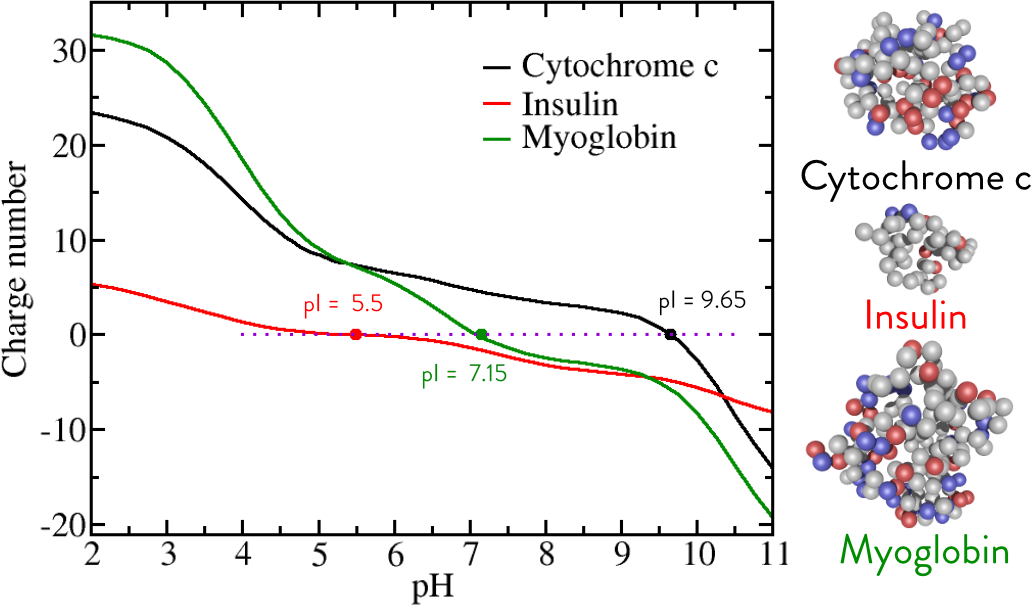
\includegraphics[width=0.65\textwidth]{Figures/graphs-gel2/protein-model.png}
     \caption{Left: Charge number of the proteins in a dilute solution as a function of  pH (solid-line curves);
     filled circles mark  the isoelectric point,
     where the net charge of the protein is zero.
     The coarse-grained representation of the proteins is illustrated on the right, where amino acid residues are represented by a single sphere (red: acidic; blue: basic; gray: charge-neutral residues).}
     \label{fig:esf:protein-charge}
 \end{figure}






 





%%%%%%%%%%%%%%%%%%%%%%%%%%%%%%%%%%%%%%%%%%%%%%%%%%
\subsection{Molecular model: Nanogel Network}
%%%%%%%%%%%%%%%%%%%%%%%%%%%%%%%%%%%%%%%%%%%%%%%%%%

Besides the protein model presented in sec.  \ref{sect:protein},   we need to specify a molecular model to describe the polymer network that makes the nanogel backbone.
Such model must provide  a set of molecular configurations of the polymer network that is representative of the whole conformational space.
A particular network conformation is given by the spacial position of all its segments.


The nanogel network is composed of 25 segment-long  crosslinked polymer chains. 
In total this network contains 10054 segments.
Each segment is a coarse-grained   representation of either a crosslink, a charge neutral unit (VA) or an acid/basic monomer (MAA/AH). 
tabla \ref{table:Coarse-grain} includes the volume and pKa (if the unit is titratable) used to describe these coarse-grained units.

The polymer network has diamond-like topology, where  crosslinks are placed at the original position of carbon atoms and connected to four polymer chains.
To build this network, we first construct a three-dimensional structure where all the polymer chains are elongated, to then only keep the segments contained within a sphere of radius $R_{cut}$ placed at the center of mass of the structure; $R_{cut}$ is selected such that the network will have 10000 segments approximately.
Originally, all polymer chains connect two crosslinks, but as a result of this procedure some will be left dangling on the network surface,  connected to a single crosslink.
Most of these superficial \emph{dangling} chains are shorter than 25 segments.
Altogether these chains contain 22\% of the total number of segments.
To generate the different molecular conformations of the polymer network, we have performed Molecular Dynamics simulations using GROMACS 5.1.2 \addcite[indahl2001gromacs] (details are given in the SI).

 \begin{figure}[!htb]
     \centering
     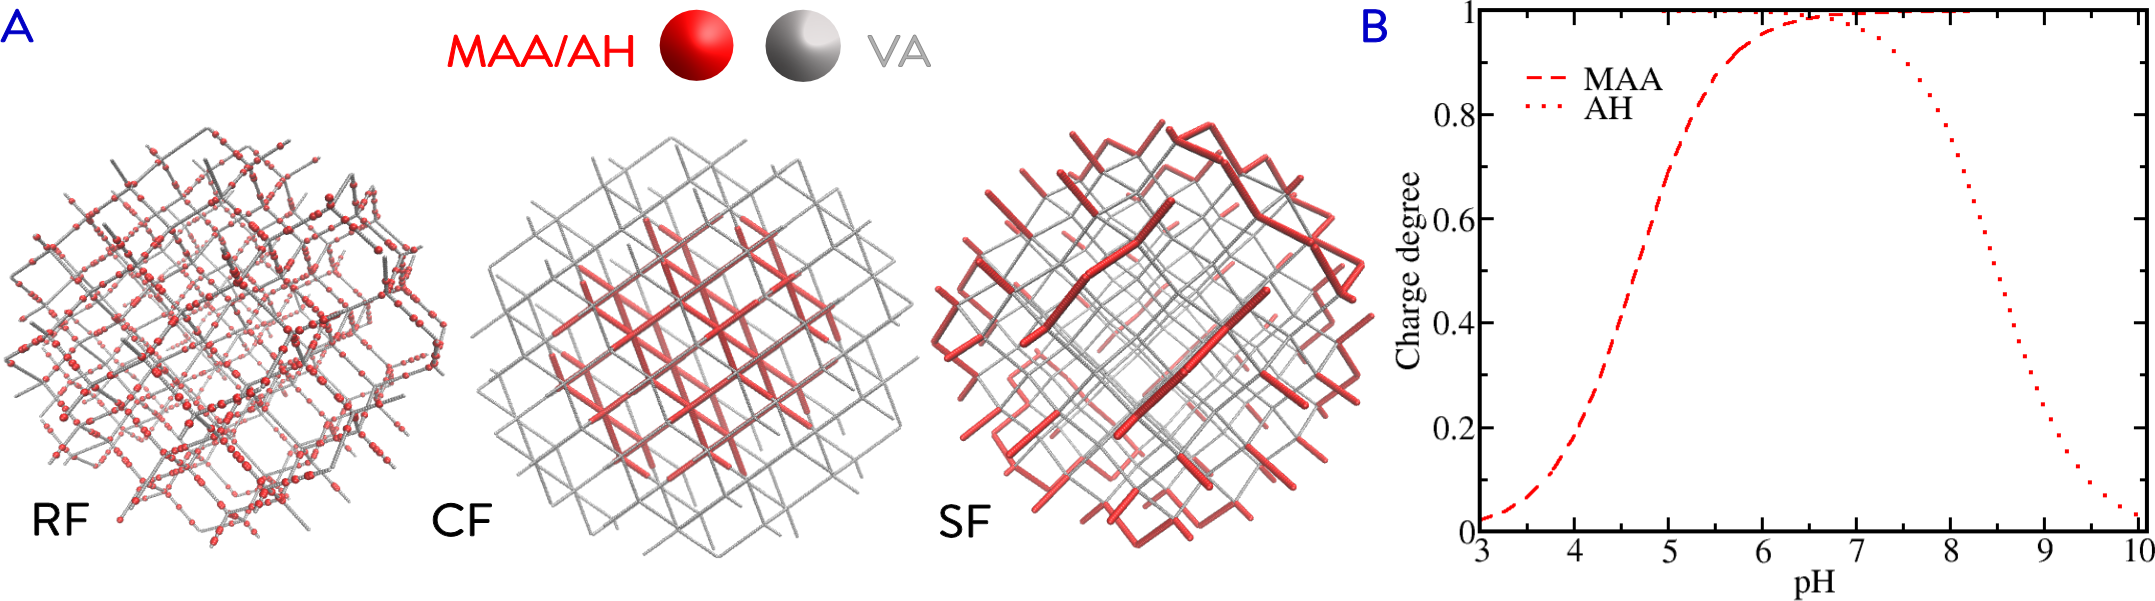
\includegraphics[width=0.99\textwidth]{Figures/graphs-gel2/paper2.png}
     \caption{A: The nanogel network consists of crosslinked copolymer chains of a charge-neutral segment (VA: vinyl alcohol) and a functional unit (either MAA: methacrylic acid or AH: allylamine).
    This scheme illustrates the three different comonomer distributions considered;  from left to right: RF: a random distribution of functional groups throughout the network; CF: the functional units occupy the center/core of the network; SF: only the free-end dangling chains on the network surface are functionalized with pH-responsive units.
B: Plot of the ideal pH-dependent degree of charge of the isolated functional unit in dilute solution.}
     \label{fig:esf:gel-topologies}
 \end{figure}














We consider different pH-responsive nanogels, containing either acid (MAA) or basic (AH) groups, and evaluate three different topologies for the spatial distribution of these functional  segments, which are schematized in figura \ref{fig:esf:gel-topologies}: 
(i) a \emph{randomly functionalized} (RF) structure where the pH-responsive segments are spread throughout the network  at random,
(ii) a \emph{core functionalized} (CF) structure, where the  pH-sensitive units occupy the center of the network, and 
(iii) a \emph{surface functionalized} (SF) structure in which only the dangling chains on the network surface  are ionizable. 

 
 
  







%%%%%%%%%%%%%%%%%%%%%%%%%%%%%%%%%%%%%%%%%%%%%%%%%%
\section{Results and discussion}
%%%%%%%%%%%%%%%%%%%%%%%%%%%%%%%%%%%%%%%%%%%%%%%%%%






%%%%%%%%%%%%%%%%%%%%%%%%%%%%%%%%%%%%%%%%%%%%%%%%%%
\subsection{Caraterizaci\'on del nanogel}
%%%%%%%%%%%%%%%%%%%%%%%%%%%%%%%%%%%%%%%%%%%%%%%%%%
En esta primera instancia  examinaremos  el comportamiento (la respuesta) de los nanogeles en funci\'on del pH en ausencia de  prote\'inas. 

Para cuantificar el tama\~no de un nanogel, usaremos el radio  de la partí\'icula, $R$, que se puede calcular usando:
\begin{align}
    R= \frac{4}{3}\frac{\int_0^\infty{dr\,G(r)\,r \left<\phi(r)\right>}}{\int_0^\infty{dr\,G(r)\left<\phi(r)\right>}}
\end{align}
donde $r$ es la distancia desde el centro de masa de la red polim\'erica (en nuestra teor\'ia asume simetr\'ia radial);
$\left<\phi(r)\right>$ es la fracci\'on de volumen local del pol\'imero (incluye todos los tipos de segmentos);
los corchetes angulares indican el promedio de ensamble sobre las diferentes conformaciones de la red (ver ecuaci\'on \ref{eq:esf:ensamble-gel});
$G(r)=4\pi r^2$ es el  \'area de la supercie de una esfera de radio $r$.

\begin{figure}[!htb]
     \centering
     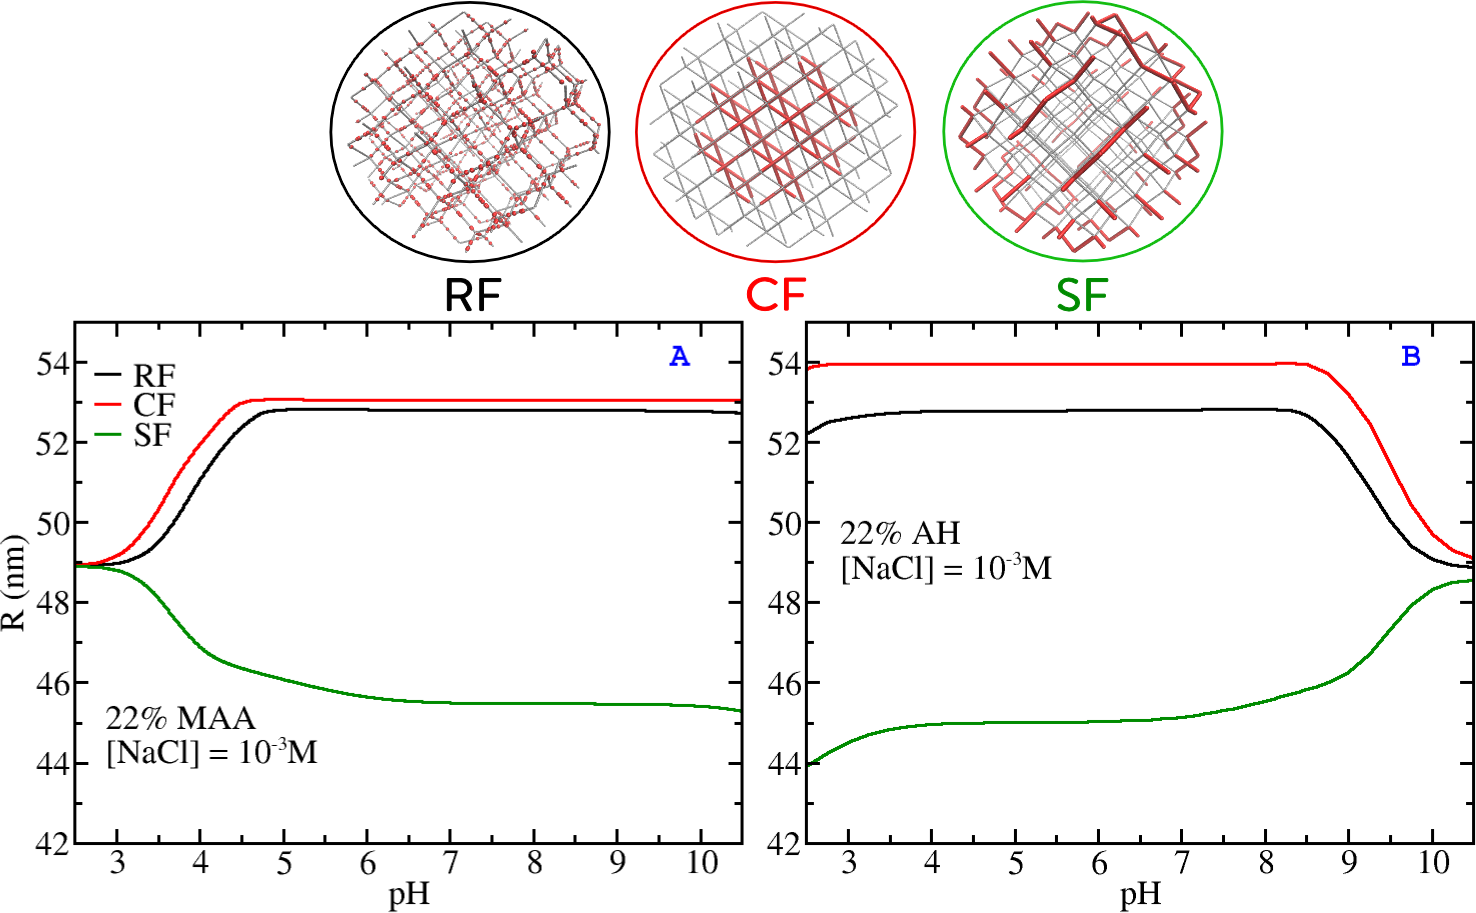
\includegraphics[width=0.9\textwidth]{Figures/graphs-gel2/rr.png}
     \caption{Radio promedio, R, en funci\'on del pH para nanogeles de copol\'imero MAA-VA (panel A) y AH-VA (panel B).
     	Se consideran tres estructuras diferentes en cada caso donde las unidades funcionales (MAA/AH) se distribuyen aleatoriamente a lo largo de la red polim\'erica (RF), ocupan el centro de la red (CF), o modifican las cadenas colgantes dentro del pol\'imero. interfaz de soluci\'on (SF).
     	En todos los casos, el $22\%$ de los segmentos de estas redes son sensibles al pH; La concentraci\'on de NaCl es $10^{-3}M$.}
     \label{fig:esf:gel-charge-MAA-AH}
\end{figure}

La Figura \ref{fig:esf:gel-charge-MAA-AH} muestra el radio promedio $R$ en funci\'on del pH para las tres diferentes estructuras consideradas: RF, CF y SF.
El panel A describe un nanogel cuyo segmeto ionizables es el $MAA$ , mientras que el panel B describe un nanogel basado en $AH$.
En ambos casos, la concentraci\'on de sal es de 1\,mM, y la fracci\'on de mon\'omero funcional ($MAA$ o $AH$) es de $22\%$.
Los nanogeles basados en $MAA$ funcionalizados al azar (RF) y en el n\'ucleo (CF) se hinchan al aumentar el pH (panel A).
Esto se debe a que los segmentos $MAA$ se desprotonan y se cargan el\'ectricamente a medida que aumenta el pH (ver figura \ref{fig:esf:gel-topologies}B), lo que da como resultado repulsiones electrost\'aticas dentro de la red.
La distancia entre las unidades $MAA$ cargadas debe aumentar para reducir estas interacciones repulsivas, con lo cual la red aumenta su tama\~no para colocar estos segmentos cargadis m\'as separados.
Resumiendo, para disminuir la repulsi\'on entre unidades $MAA$ cargadas, su distancia espacial debe aumentar, lo que resulta en una expansión neta de la red.




La red $MAA$ funcionalizada en  su superficie, por otro lado, muestra un comportamiento de expansi\'on completamente diferente, vease en figura \ref{fig:esf:gel-charge-MAA-AH}A.
Este nanogel se deshincha a medida que las unidades titulables se cargan al aumentar el pH.
Para explicar este comportamiento contrario a lo que se espera, observamos la distribuci\'on local de segmentos dentro de nuestras estructuras en diferentes condiciones. Utilizamos la distribuci\'on radial de los mon\'omeros funcionales.
Para los nanogeles $MAA$, dicha cantidad se define como:

%
\begin{align}
    \lambda_{MAA}(r)= 4\pi r^2\left<\phi_{MAA}(r)\right>
\end{align}
%
\noindent en donde $\left<\phi_{MAA}(r)\right>$ da la fracci\'on de volumen local de los segmentos de \'acido metacr\'ilico.
Hay que tener en cuenta que $\lambda_{MAA}(r) dr$ da el n\'umero de segmentos MAA en la capa esf\'erica entre $r$ y $r+dr$ medidos desde el centro del nanogel.
Adem\'as, la integral $\int_0^\infty \lambda_{MAA}(r) dr$ da el n\'umero total de mon\'omeros MAA en la red.


\begin{figure}[!htb]
     \centering
     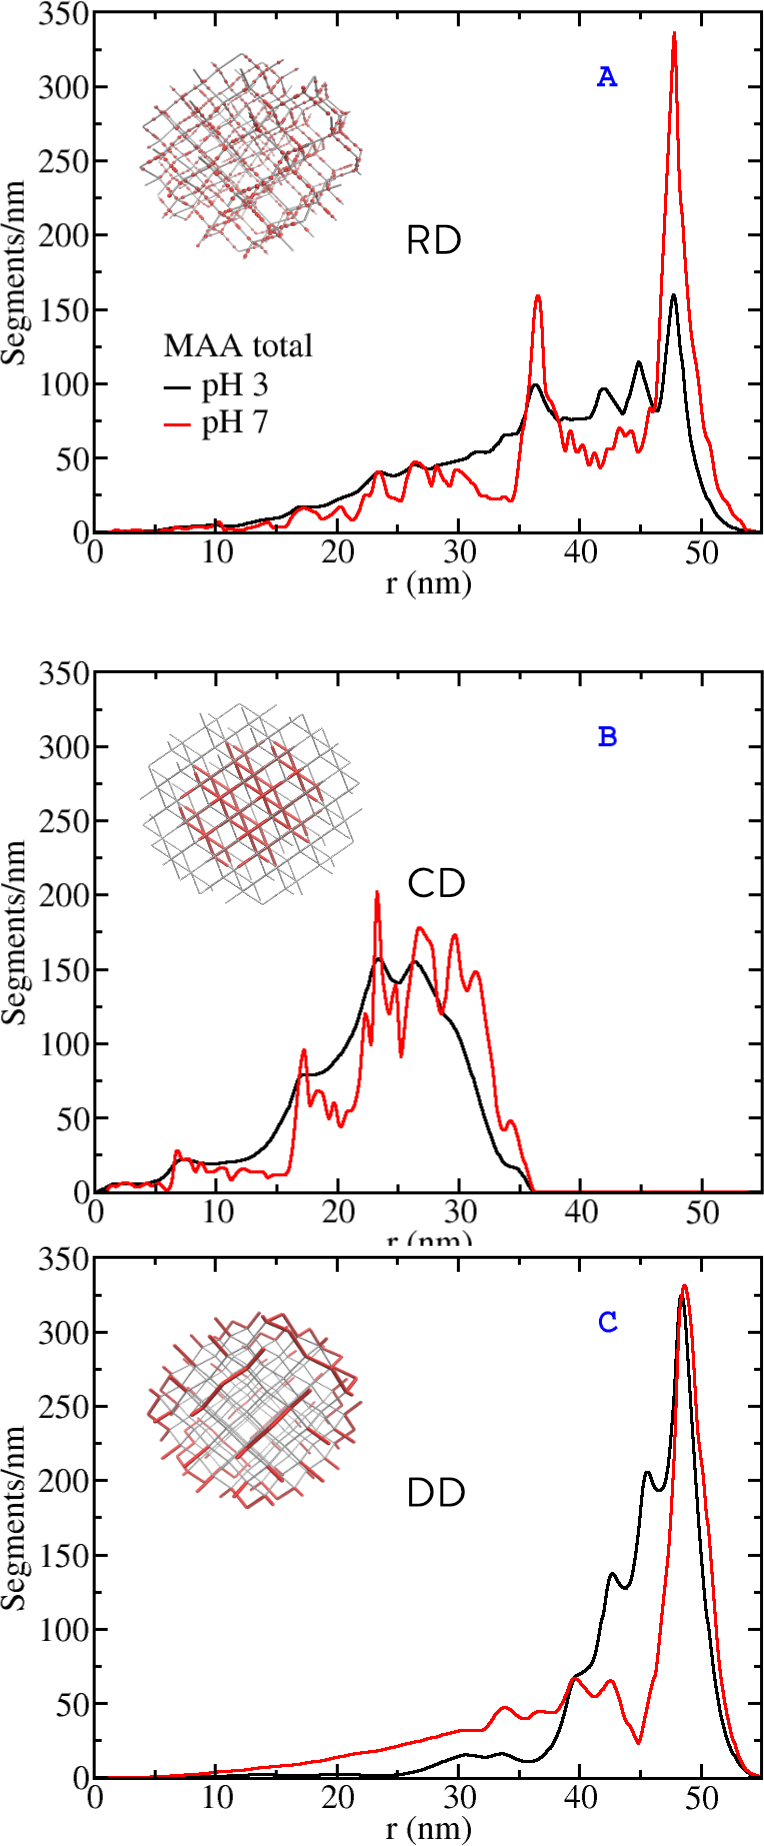
\includegraphics[width=0.45\textwidth]{Figures/graphs-gel2/dist-MAA.png}
     \caption{Distribuci\'on radial de segmentos MAA, $\lambda_{MAA}(r)$, a pH 3 y 7, y $10^{-3}M$ NaCl; cada panel corresponde a un nanogel de  MAA-VA diferente que tienen una funcionalizaci\'on de red particular y 22\% MAA.
     	Estos grupos funcionales est\'an completamente protonados (sin carga) a pH 3 y completamente disociados (cargados) a pH 7.}
     \label{fig:esf:MAA-vs-r-distribution}
 \end{figure}
 %\FloatBarrier


La figura \ref{fig:esf:MAA-vs-r-distribution} muestra la distribuci\'on radial de los segmentos de $MAA$ para las diferentes redes consideradas.
En cada caso se incluyen  resultados para una soluci\'on de pH 3, donde los segmentos $MAA$ tienen carga neutra, y pH 7 donde est\'an completamente cargados (ver figura \ref{fig:esf:gel-topologies}B);
Para una funcionalizaci\'on aleatoria (panel A), la distribuci\'on de los segmentos $MAA$ se desplaza hacia la interfaz de soluci\'on del nanogel a medida que la red se carga el\'ectricamente cuando aumenta el pH.
Este desplazamiento se produce para reducir las repulsiones electrost\'aticas entre los segmentos $MAA$ cargados.

Como resultado, toda la distribuci\'on del pol\'imero tambi\'en se extiende %(ver \cref*{fig:allseg_si}\hl{A y B en el SI})
, incluidas las unidades VA de carga neutra.  ver figura \ref{fig:esf:allr-distribution}.
El mismo comportamiento tiene lugar para una funcionalizaci\'on central (panel \ref{fig:esf:MAA-vs-r-distribution}B),
aunque por dise\~no, los segmentos $MAA$ en esta red, ya sea que est\'en cargados o no, es m\'as probable que ocurran a distancias m\'as cortas del centro del nanogel en comparaci\'on con las otras estructuras.
El desplazamiento de segmentos a $r$ m\'as altos observado en los paneles figura \ref{fig:esf:MAA-vs-r-distribution}A y B explica el aumento del tama\~no promedio del nanogel con pH visto en la figura \ref{fig:esf:gel-charge-MAA-AH}A para las estructuras RF y CF.


Por otro lado, la figura \ref{fig:esf:MAA-vs-r-distribution}C muestra que la distribuci\'on superficial de segmentos de $MAA$ se desplaza hacia adentro cuando la red se carga con el aumento de pH.
Para reducir las repulsiones dentro de la red, las cadenas libres (de la superficie) de $PMAA$ , que se asientan en la superficie del nanogel a un pH bajo, tambi\'en intentan ocupar el volumen dentro de la red cuando están cargadas.
Este cambio hacia adentro de la distribuci\'on de segmentos de pol\'imero (\ref{fig:esf:allr-distribution}C)
explica el comportamiento de deshinchamiento del nanogel tipo SF con el aumento del pH que se observa en la figura \ref{fig:esf:gel-charge-MAA-AH}A.
N\'otese, sin embargo, que a pesar de este desplazamiento parcial hacia el interior de la red, la posici\'on m\'as probable de los segmentos MAA es siempre la interfaz pol\'imero-soluci\'on para soluciones de pH alto y bajo. Al empujar toda la estrucutura hacia dentro del nanogel los segmentos de $MAA$ quedan igualmente expuestos.



El comportamiento de los nanogeles compuestos por $AH$ es an\'alogo al de las redes basadas en $MAA$, pero en respuesta al cambio de pH en la direcci\'on opuesta.
Los grupos $AH$ se protonan y se cargan positivamente con la disminuci\'on del pH (ver figura \ref{fig:esf:gel-topologies}B).
Para nanogeles de $AH$ funcionalizados aleatoriamente y en su n\'ucleo, este aumento en la carga el\'ectrica con la disminución del pH provoca un desplazamiento hacia afuera de la distribuci\'on del segmento. Del mismo modo que se observ\'o para los nangoles compuestos por $MAA$% (ver \cref*{fig:AHseg_si}A y B)
, lo que explica la hinchaz\'on de la figura \ref{fig:esf:gel-charge-MAA-AH}B;
mientras tanto, para la estructuratipo SF, el deshinchamiento con la disminuci\'on del pH que se ve en la figura \ref{fig:esf:gel-charge-MAA-AH}B es consistente con un desplazamiento hacia adentro del pol\'imero %(ver \cref*{fig:AHseg_si}C) .


La figura \ref{fig:esf:allr-distribution} muestra la distribuci\'on de todos los segmentos que componen la red polim\'erica de los diferentes nanogeles. 
Al igual que en fig. \ref{fig:esf:MAA-vs-r-distribution} presentamos la distribuci\'pn para dos diferentes valores de pH. Que corresponde a los estados protonado (pH 3 ) y desprotonado (pH 7) de los segmentos de $MAA$.  En los paneles A y B se observa un aumento de cantidad de segmentos a valores m'as altos de $r$ al cargarse el nanogel. Comportamiento observado en la figura \ref{fig:esf:gel-charge-MAA-AH}, en donde hay un aumento del radio del nanogel (RF y CF).
En cambio el desplazamiento hacia dentro de los segmentos de la red polim\'erico al transicionar de un estado cargado a uno descargado en la distribuci\'on superficilal (SF) explica la disminuci\'on del tama\~no del gel observada en la figura \ref{fig:esf:gel-charge-MAA-AH}B.

\begin{figure}[!htb]
	\centering
	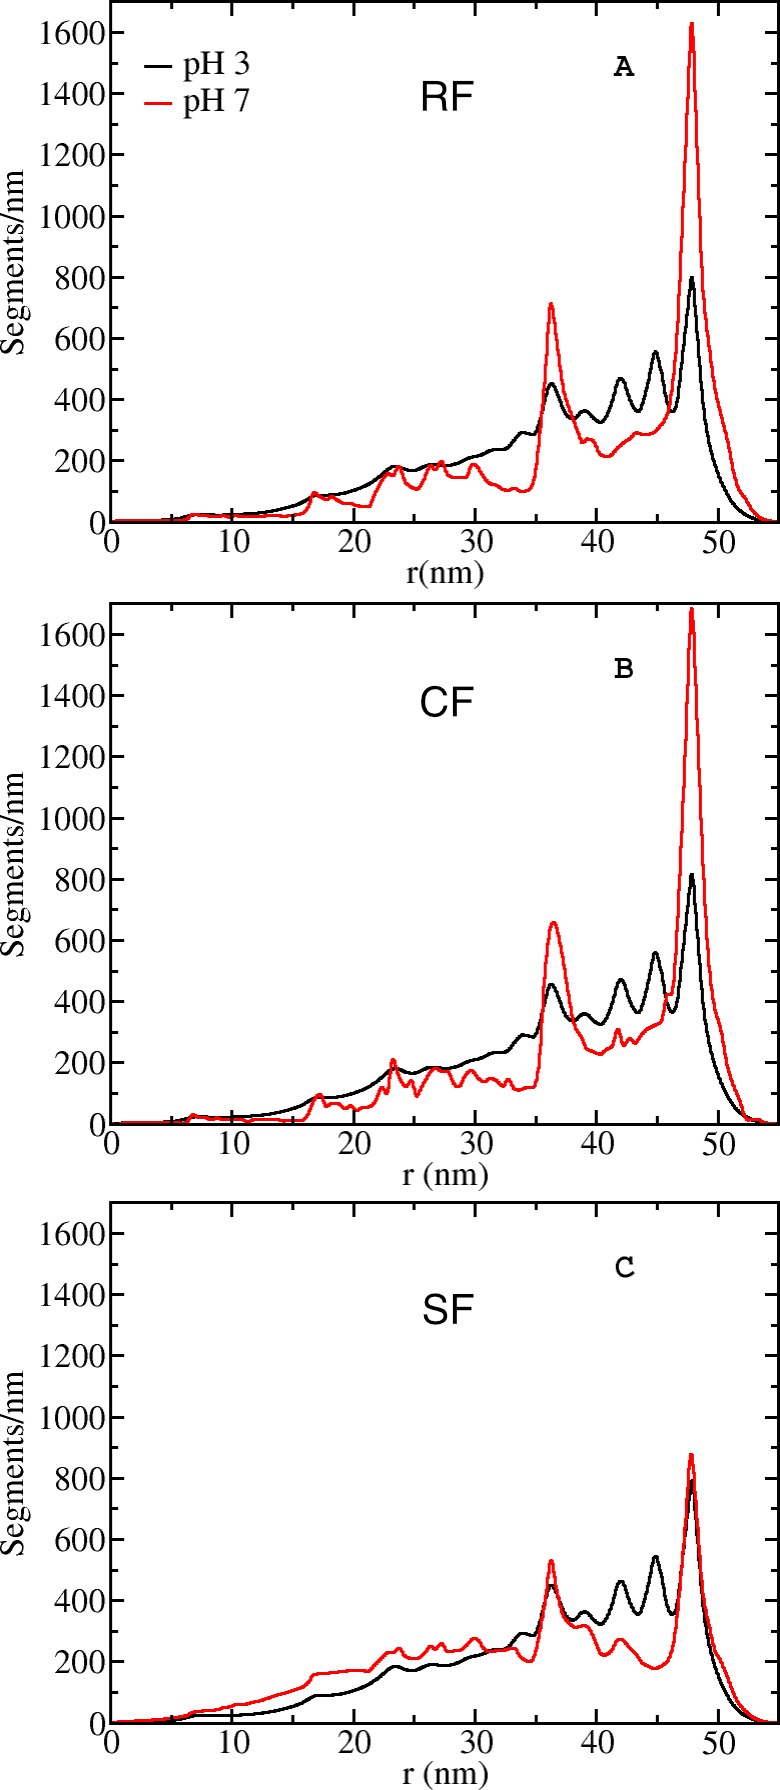
\includegraphics[width=0.45\textwidth]{Figures/graphs-gel2/allseg_SI.png}
	\caption{Distribuci\'on radial detodo los segmentos que componene la estructura del nanogel, $\lambda(r)$, a pH 3 y 7, y $10^{-3}M$ NaCl; cada panel corresponde a una funcionalizaci\'on  diferente}
	\label{fig:esf:allr-distribution}
\end{figure}




%%%%%%%%%%%%%%%%%%%%%%%%%%%%%%%%%%%%%%%%%%%%%%%%%%
\subsection{Protein adsorption to MAA-based nanogels}\label{sec:MAA-NGs}
%%%%%%%%%%%%%%%%%%%%%%%%%%%%%%%%%%%%%%%%%%%%%%%%%%



%%%%%%%%%%%%%%%%%%%%%%%%%%%
%%%%% Define Gamma and N(r)
%%%%%%%%%%%%%%%%%%%%%%%%%%%

En la secci\'on anterior se  evalu\'o el impacto de la funcionalizaci\'on de la red y la composici\'on qu\'imica en la respuesta del nanogel a las variaciones de pH en ausencia de prote\'inas.

La reorganizaci\'on de los segmentos de la red polim\'erica es resultado de los cambios en el pH con una dependencia en la elecci\'on de dise\~no: es decir la distribuci\'on de unidades funcionales dentro de la red.

En esta parte se mostrara el impacto de esta reorganizaci\'on de la red  polim\'erica en el nivel de adsorci'on de prote\'inas en diferentes nanogeles, as\'i como la distribuci\'on espacial de las prote\'inas adsorbidas.

En particular mostramos el an\'alisis de la adsorció\'on del citocromo c y mioglobina en diferentes estructuras de nanogeles basados  en $MAA$.
Adem'as mostraremos estudios de adsroci\'on de insulina, pero en este caso con nangoles teniendo $AH$ como segmento protonable.
Los resultados de la insulina con $MAA$ se omiten debido a su bajo punto isoel\'ectrico, esta prote\'na no se adsorbe en nanogeles basados en $MAA$.  

Para estos estudios vamos a condierar a un nanogel polim\'erico centrado en $r=0$ en contacto con una soluci\'on acuosa de prote\'ina.
El n\'umero de prote\'inas adsorbidas dentro de la capa esf\'erica entre $r$ y $r+dr$ viene dado por la cantidad en exceso, definida: 

\begin{align}
     \langle N(r)\rangle dr = 4\pi r^2 \left(\langle\rho(r)\rangle - \rho_{bulk}\right) dr
\end{align}
%
en donde $\left<\rho(r)\right>$ y $\rho_{bulk}=\lim\limits_{r\to \infty } \langle\rho(r)\rangle$ son respectivamente la densidad (en n\'umero) local y en el bulk de la prote\'ina.
La integraci\'on de $\langle N(r)\rangle$ produce la \emph{adsorci\'on en exceso} (en adelante, simplemente la adsorci\'on) que cuantifica el n\'umero de prote\'inas incorporadas a la red de pol\'imeros,


%
\begin{align}
    \Gamma =  \int_0^\infty{  \langle N(r)\rangle dr}
\end{align}
%

%%%%%%%%%%%%%%%%%%%%%%%%%%%
%%%%% Adsorption to MAA NGs
%%%%%%%%%%%%%%%%%%%%%%%%%%%


\begin{figure}[!htb]
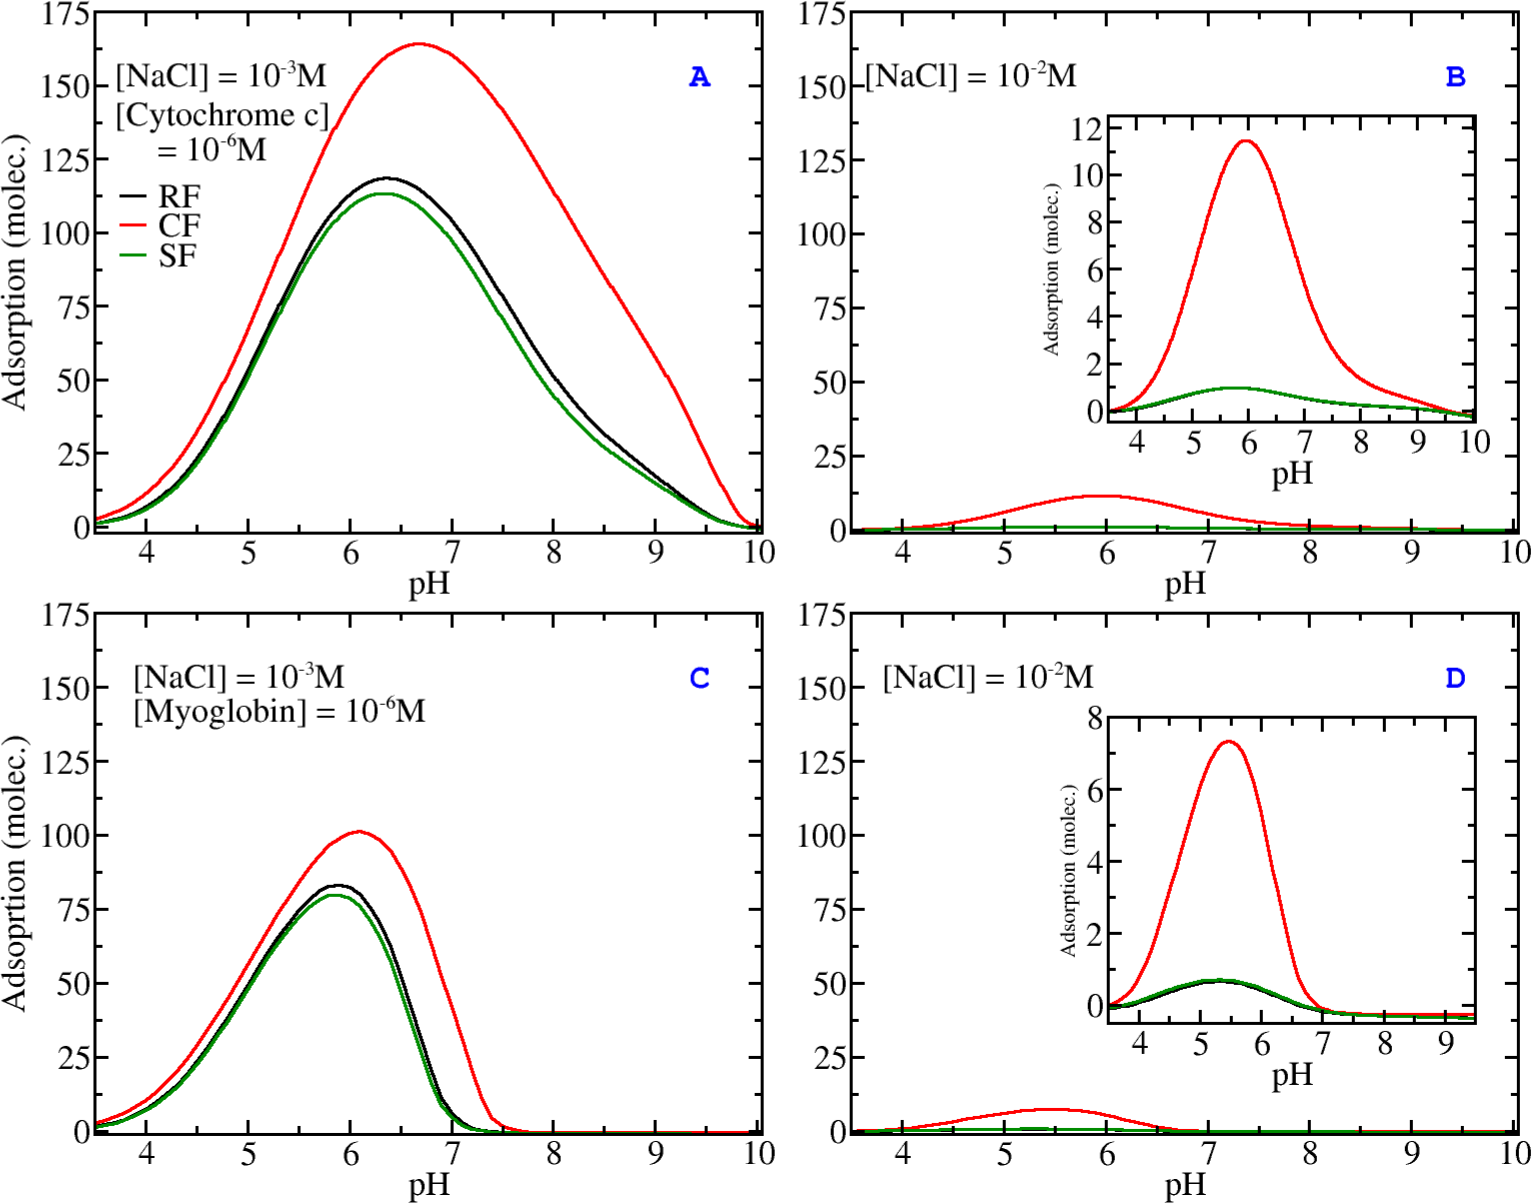
\includegraphics[width=0.9\textwidth]{Figures/graphs-gel2/abcd.png}
\caption{Gr\'aficos del exceso de adsorci\'on $\Gamma$ de citocromo c (paneles A y B) y mioglobina (paneles C y D) a nanogeles MAA-VA en funci\'on del pH.
	La concentraci\'on de sal es $10^{-3}M$ en los paneles del lado izquierdo (A y C) y $10^{-2}M$ en los paneles del lado derecho
	(B y D); Se muestra una ampliaci'on de la adsorci\'on.
	Estos nanogeles tienen 22\% MAA; la concentraci\'on de prote\'ina es $10^{-6}M$.}
\label{fig:esf:adsorption-vs-pH-cyto-myo}
\end{figure}



 
 La Figura \ref{fig:esf:adsorption-vs-pH-cyto-myo} muestra la adsorci\'on de soluciones de prote\'ina \'unica de citocromo c (paneles superiores, A y B) y mioglobina (paneles inferiores, C y D) en nanogeles de $MAA-VA$ con difrente funcionalizaci\'on en su red;
 El pH es la variable independiente de estos c\'alculos, pero tambi\'en evaluamos el efecto de la concentraci\'on de NaCl comparando diferentes paneles en la misma l\'inea.
 Los nanogeles de Figura \ref{fig:esf:adsorption-vs-pH-cyto-myo} contienen $22\%$ en $MAA$, para los nanogeles funcionalizados en su superficie significa que todos los segmentos en las cadenas superficiales de la red estan compuestos por $MAA$.
  
 
 Puede observarse que la adsorci\'on de prote\'inas es una funci\'on no monot\'onica del pH con un m\'aximo en la regi\'on entre pH 5-7, que depende de la concentraci\'on de sal y la prote\'ina espec\'ifica.
 Esta respuesta del pH puede explicarse en t\'erminos de las interacciones electrost\'aticas y el comportamiento de protonaci\'on tanto de los segmentos de $MAA$ como de las prote\'inas.
 Las unidades \'acidas del pol\'imero se disocian y la red se carga negativamente cuando el pH aumenta por encima de su pKa intr\'inseco (4,65 para MAA).
 Por encima de este pH, pero por debajo de su punto isoel\'ectrico, la prote\'ina tiene carga positiva.
 En estas condiciones, las atractivas interacciones prote\'ina-red impulsan la adsorci\'on.
 Sin embargo, en ambos lados de la escala de pH, estas interacciones son insignificantes (pH bajo) porque el MAA est\'a protonado y tiene carga neutra o repulsivo (pH alto) porque las prote\'inas tienen carga negativa.
 Cualquiera de las dos situaciones conduce a la ausencia de adsorci\'on de prote\'inas ($\Gamma\approx 0$) o desorci\'on ($\Gamma< 0$).
 
 
 
 En general, las adsorciones de citocromo c y mioglobina son cualitativamente similares.
 Hay dos diferencias principales: (i) la magnitud de la adsorci\'on (el citocromo c se adsorbe significativamente m\'as) y (ii) el citocromo c se adsorbe en un rango de pH m\'as amplio, lo que se debe a su punto isoel\'ectrico m\'as alto (9,65 en comparaci\'on con 7,15). para la mioglobina).
 Esto tambi\'en implica que, cuando las dem\'as condiciones son las mismas, el nivel m\'aximo de adsorci\'on de citocromo c tiene lugar a un pH ligeramente superior.
 
 En relaci\'on con las otras configuraciones, la figura \ref{fig:esf:adsorption-vs-pH-cyto-myo} muestra que la distribuci\'on central de los segmentos MAA conduce a una adsorci\'on significativamente mayor en la mayor\'ia de las condiciones.
 Mostramos que este comportamiento ocurre porque tal distribuci\'on de segmentos MAA permite una incorporaci\'on m\'as efectiva de la prote\'ina adsorbida con carga el\'ectrica opuesta.
 Por otro lado, el comportamiento de adsorci\'on de las redes funcionalizadas aleatoriamente y de superficie es sorprendentemente similar dentro del pH y las concentraciones de sal estudiadas, y tambi\'en para las diferentes prote\'inas.
 La distribuci\'on de unidades funcionales entre estructuras RF y SF difiere mucho a pH bajo.
 Sin embargo, tras la reorganizaci\'on del polí\'imero a un pH m\'as alto a medida que se cargan las unidades MAA, estas distribuciones se vuelven relativamente similares entre s\'i (compare los paneles A y C de la Figura \ref{fig:esf:MAA-vs-r-distribution}), lo que explica la adsorci\'on de prote\'inas comparable observado en nanogeles RF y SF.




%%%%%%%%%%%%%%%%%%%%%%%%%%
%%%%% Protein localization
%%%%%%%%%%%%%%%%%%%%%%%%%%

\begin{figure}[!htb]
     \centering
     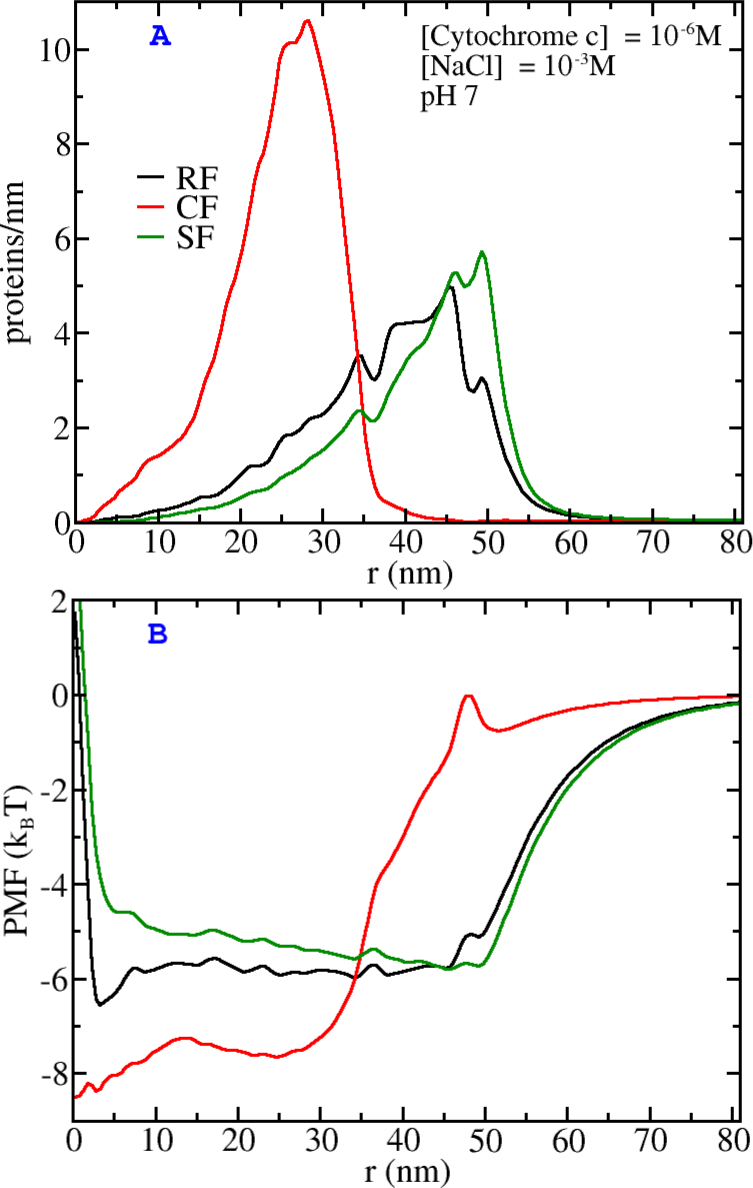
\includegraphics[width=0.45\textwidth]{Figures/graphs-gel2/cyto-adsr-pmf.png}
     \caption{Panel A: Gr\'afico de la distribuci\'on radial de las mol\'eculas de citocromo c, $\langle N(r)\rangle$, en funci\'on de la posici\'on de los nanogeles MAA-VA con diferentes funcionalizaciones.
     	Estas redes tienen 22\% MAA, el pH es 7, la concentraci\'on de prote\'ina es de $10^{-6}M$ y la concentraci\'on de NaCl es de $10^{-3}M$.
     	El panel B muestra el potencial de la fuerza media, ${PMF}(r)$, que act\'ua sobre el citocromo c para las mismas condiciones que el panel A.}
     \label{fig:esf:adsorption-vs-r-cyto}
 \end{figure}



Para explicar el mejor rendimiento de los nanogeles MAA funcionalizados con n\'ucleo en la incorporaci\'on de prote\'inas,
La figura \ref{fig:esf:adsorption-vs-r-cyto}A muestra la distribuci\'on radial de las mol\'eculas de citocromo c en funci\'on de la distancia $r$ al centro de masa del nanogel.
La soluci\'on tiene pH 7 y NaCl 1\,mM, lo que corresponde aproximadamente a las condiciones de m\'axima adsorci\'on de esta prote\'ina en la Figura \ref{fig:esf:adsorption-vs-pH-cyto-myo}A.
Existe una clara correlaci\'on entre la distribuci\'on de los grupos funcionales a lo largo de la red polim\'erica y la ubicaci\'on del citocromo c adsorbido.



When the center of the network is functionalized, the highest probability of finding the proteins occurs deep inside the nanogel between 20-30\,nm.
In Figura \ref{fig:esf:adsorption-vs-r-cyto}A the maximum number of adsorbed proteins occurs at $r=28$\,nm for $1$\,mM NaCl, and at $r=25$\,nm for 10\,mM NaCl% (\hl{see} \cref*{fig:cyto-vs-r-1d-2_si}).
Congruently, the distribution profile of charged MAA displays a shallow maximum in this spatial region (see figura \ref{fig:esf:MAA-vs-r-distribution}B, red curve).
Namely, adsorbed proteins sit where they can be surrounded by oppositely charged network segments.
Interestingly, the same phenomenon takes place in the adsorption to RF and SF nanogels.
The distributions of charged MAA display a sharp maximum near the nanogel surface, between 45-50\,nm (see red curves in  figura \ref{fig:esf:MAA-vs-r-distribution}, panels A and C).
Fig 6A shows that cytochrome c is most likely to adsorb next to these  regions of high MAA (charge) density.



When comparing the distributions of cytochrome c inside RF and SF nanogels in figura \ref{fig:esf:adsorption-vs-r-cyto}A, we observe that the profiles are relatively similar to each other.
As expected, if only the surface is functionalized, the protein profile shifts towards the polymer-solution interface.
To further quantify the interaction with the nanogels, we use the potential of mean force acting on a protein at a distance $r$ from the center of the polymer network, defined as:
\begin{align}
   {PMF} (r) = -k_B T \ln \frac{\langle \rho(r)\rangle}{\rho_{bulk}}
\end{align}
where $\lim\limits_{r\to \infty}{PMF}(r)=0$, which means that the nanogel-protein interaction vanishes when they are sufficiently far apart.





Figura \ref{fig:esf:adsorption-vs-r-cyto}B shows ${PMF}(r)$ acting on cytochrome c at the same conditions of panel A, and for the three different nanogel functionalizations.
Deep inside the nanogel, protein interaction with the CF structure is the strongest: $-8k_B T$ approximately in the spatial range from $r=0$ to 30\,nm.
This interaction is relatively short-ranged because it decreases significantly above $r approx 40$\,nm.
On the other hand,  cytochrome c interactions with RF and SF nanogels extend longer, up to $55-60$\,nm.
Inside the nanogel, these interactions are weaker than that with the CF structure.
The adsorption free energy is $\sim -6 k_BT$ and it remains roughly constant inside the RF nanogel.
For the surface-functionalized nanogel, on the other hand, the minimum of ${PMF}(r)$ is also $\sim -6 k_BT$, occuring next to the polymer-solution interface ($r\approx 50$\,nm).
As opposed to the RF structure, this interaction is not constant inside the nanogel, but it increases monotonously as $r$ decreases and the protein gets further away from the functionalized superficial dangling chains.












%%%%%%%%%%
%%%% change in salt

\begin{figure}
     \centering
     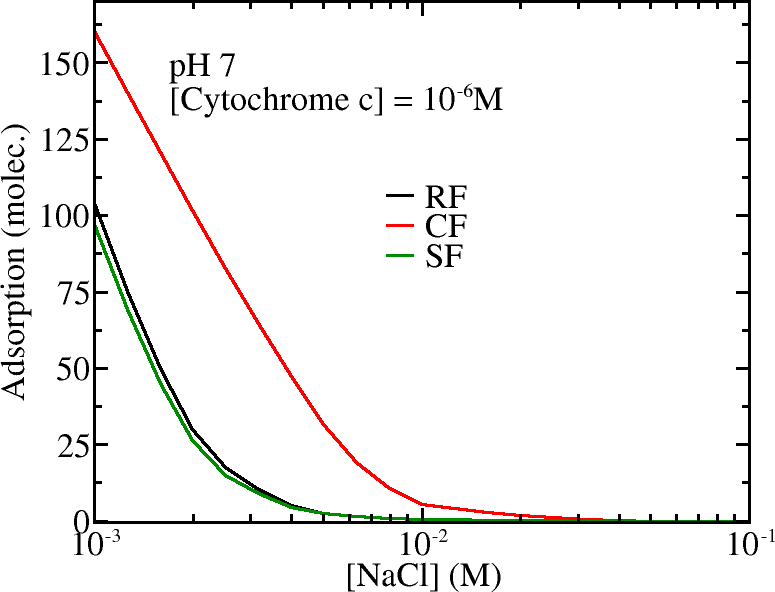
\includegraphics[width=0.45\textwidth]{Figures/graphs-gel2/gamma-salts-cyto.png}
     \caption{Plot of the excess adsorption $\Gamma$ of cytochrome c as a function of salt concentration at pH 7 for MAA-VA nanogels with different network functionalizations having 22\% MAA; protein concentration is $10^{-6}M$.}
     \label{fig:esf:adsorption-vs-salt-cyto}
 \end{figure}
 

A feature of protein adsorption that we have not fully discussed yet is the effect of salt concentration.
For both cytochrome c and myoglobin, figura \ref{fig:esf:adsorption-vs-pH-cyto-myo} shows that the incorporation of proteins inside the different nanogels is significantly enhanced by decreasing the solution salt concentration.
In order further characterize this behavior in  figura \ref{fig:esf:adsorption-vs-salt-cyto} presents cytochrome c adsorption as a function of NaCl concentration at pH 7. 
This graph shows that all network functionalizations display a qualitatively similar behavior, with a dramatic decrease in adsorption between 1 and 10\,mM NaCl.
At 100\,mM all nanogels show negligible or negative adsorption.

When the solution salt concentration is high, both Na$^+$ and Cl$^-$ ions are found in high concentrations inside the nanogel.
These ions screen the electrostatic attractions between the positive charges of the protein and the negative charges on the polymer, which are the driving force for protein adsorption.
Effectively, these attractions become short range and are not strong enough to result in significant if any protein adsorption.
If the concentration of NaCl is lower, on the other hand, these electrostatic interactions are less screened and effectively longer ranged, which allows for protein adsorption.
Thus, decreasing the salt concentration enhances adsorption.
ROJO 
{Such behavior has been observed in experiments, which show that there is an increase in protein adsorption at low salt concentration \addcite[becker2012proteins, henzler2010adsorption,xu2018interaction].
Adsorption to planar and spherical polyelectrolyte brushes is significantly favored at lower salt concentrations, as demonstrated using isothermal titration calorimetry. ROJO




In considering carriers for protein delivery applications our results suggest that the best conditions for encapsulation correspond to low salt.
The adsorption profiles of figura \ref{fig:esf:adsorption-vs-salt-cyto} are qualitatively similar for the three functionalizations,
but the number of proteins inside the nanogel is always significantly larger for the CF structure.
This feature may be critical in designing delivery vehicles for a target having intermediate salt concentrations.
The CF incorporates more proteins at the same conditions, but it may not be able to release them if the target has intermediate salt concentration.
For these conditions the random functionalization will be able to release all its cargo.















%%%%%%%%%%%%%%%%%%%%%%%%%%%%%%%%%%%%%%%%%%%%%%%%%%
\subsection{Insulin adsorption AH-based nanogels} 
%%%%%%%%%%%%%%%%%%%%%%%%%%%%%%%%%%%%%%%%%%%%%%%%%%




Insulin does not adsorb to the MAA nanogels of sec.  \ref{sec:MAA-NGs} %(see \cref*{fig:adsoprtion-vs-pH-insulinMAA_si} in SI).
This is because the isoelectric point of insulin and the pKa of MAA are close to each other, meaning that for solutions where the protein is positively charged, the nanogel is charge neutral, and if the nanogel is negatively charged so is the protein.
In this context, we decided to investigate insulin adsorption to an allylamine nanogel, which is positively charged below its pKa of 9.5, overlapping with the range where insulin is negatively charged.
Other than the functional monomers, the structure of these AH-VA copolymer networks is the same as that of the MAA-VA nanogels previously described.



\begin{figure}[!htb]
    \centering
    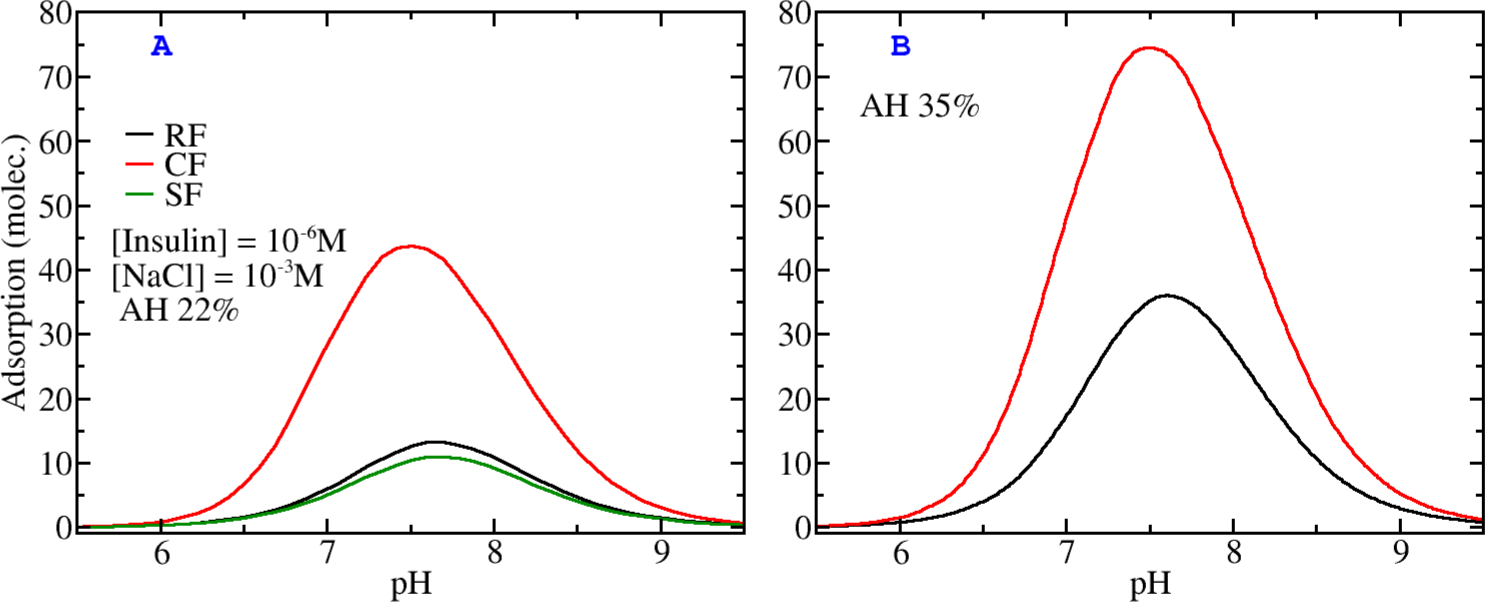
\includegraphics[width=0.9\textwidth]{Figures/graphs-gel2/insu-PAH.png}
    \caption{Plots of adsorbed insulin molecules, $\Gamma$, as a function of pH for  AH-VA nanogels having different functionalizations.
    The AH content is 22\% for the polymer networks of panel A and 35\% for those of panel B (this latter degree of functionalization cannot be achieved for the SF nanogel).
    Other conditions are $10^{-3}$\,M NaCl, and [Insulin] = $10^{-6}$\,M.}
    \label{fig:esf:adsorption-vs-pH-insulin}
\end{figure}






Figura \ref{fig:esf:adsorption-vs-pH-insulin}A shows the adsorption of insulin to AH-based nanogels having different spatial functionalizations.
Again we have considered networks with 22\% of pH-sensitive monomers so that we can include results for the SF nanogel, whose dangling chains are AH homo-polymers.
The main features of this plot are qualitatively similar to those of cytochrome c and myoglobin adsorption to the MAA nanogels (see Figura \ref{fig:esf:adsorption-vs-pH-cyto-myo}).
Namely, insulin displays a  nonmonotonic adsorption as a function of the solution pH.
Moreover, we see that the core distribution of AH segments captures more insuline than either the random or the surface functionalizations.
The RF and SF nanogels display relatively similar pH-dependent adsorption profiles.
Finally, a rising salt concentration has a critical effect on the magnitude of insulin adsorption, which is because of the increasing shielding of network-protein electrostatic attractions by mobile i


Despite the qualitative similarities between the adsorptions profiles of
Figura \ref{fig:esf:adsorption-vs-pH-insulin}A and those of cytochrome c and myoglobin (Figura \ref{fig:esf:adsorption-vs-pH-cyto-myo}A and C), we see that the number of insulin molecules captured by the AH-networks is significantly less than that of the other proteins by the MAA-based nanogels.
For this reason, we  will next evaluate the effect of the degree of functionalization of the polymer network to enhance protein adsorption.
Figura \ref{fig:esf:adsorption-vs-pH-insulin}B presents insulin adsorption for nanogels having 35\% of AH segments.
Here, the surface functionalized structure is not included because there are not enough segments in the dangling chains.
A higher HA content drives more adsorption, which results from comparing both panels of Figura \ref{fig:esf:adsorption-vs-pH-insulin}.
Once again, the CF nanogel adsorbs more insulin than the RF network (more than twice as many proteins for the conditions of this calculations).




\begin{figure}[!htb]
    \centering
    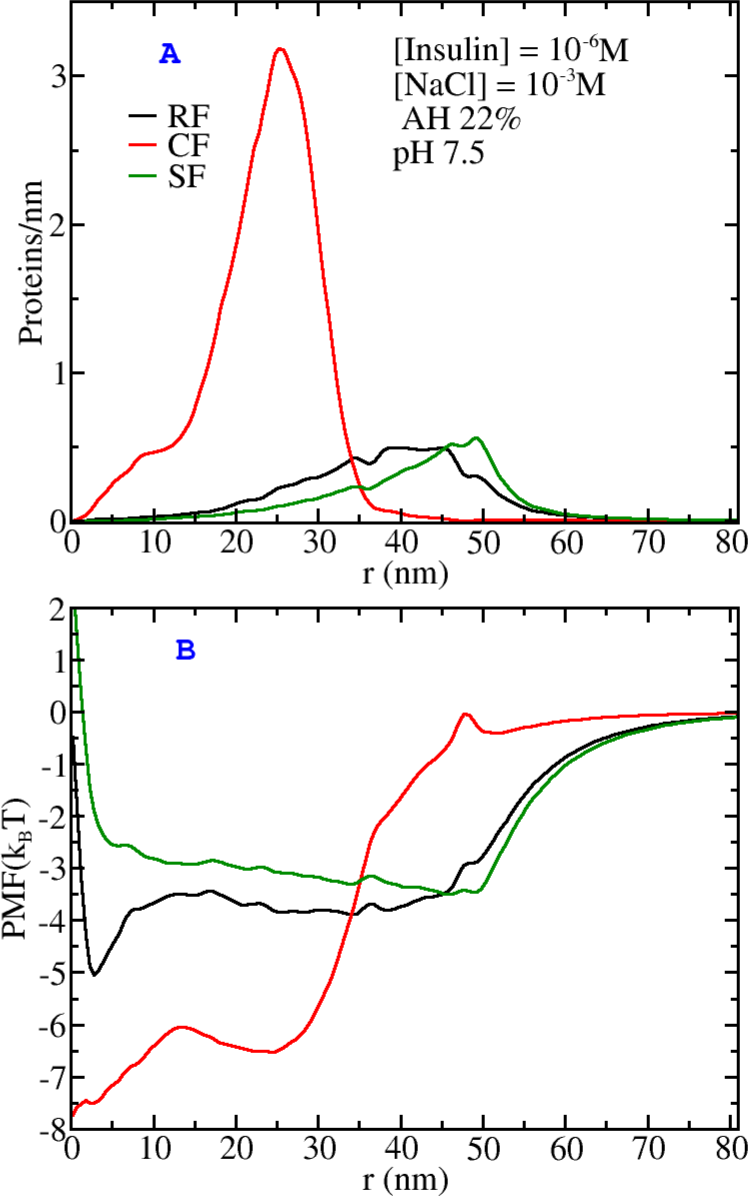
\includegraphics[width=0.45\textwidth]{Figures/graphs-gel2/insu-ads-pmf.png}
    \caption{A: Plot of the local distribution of insulin molecules, $\langle N(r)\rangle$, as a function of position for AH-VA nanogels having 22\% pH-sensitive segments in different network configurations.
    pH is 7.5, $10^{-6}$\,M insulin and  $10^{-3}$\,M NaCl.
    B: Potential of mean force,  ${PMF}(r)$, as a function of position for the same conditions as panel A.}
    \label{fig:esf:adsorption-vs-r-insulin}
\end{figure}



Figura \ref{fig:esf:adsorption-vs-r-insulin}A shows how adsorbed proteins are spatially distributed inside the different AH-based nanogels with \%22 degree of functionalization.
The pH of these results corresponds to the adsorption maximum of Figura \ref{fig:esf:adsorption-vs-pH-insulin}A.
Insulin adsorption to the CF nanogel is not only significantly higher than the adsorption to the RF and SF nanogels, but it also occurs deeper inside the structure.
The most likely position of an insulin molecule occurs around $r=25$\,nm for the CF nanogel,
while this position moves to around $40-45$ and 50\,nm for the RF and SF structures respectively.




For MAA-based nanogels, Figura \ref{fig:esf:adsorption-vs-r-cyto}A shows relatively minor differences between the distributions of cytochrome c inside RF and SF networks.
Such are differences slightly accentuated for insulin adsorption to the AH-VA nanogels, as seen in Figura \ref{fig:esf:adsorption-vs-r-insulin}A.
Insulin distribution is displaced to the interior of the network in the randomly modified nanogel as compared to the surface functionalization, where proteins are more likely to occupy the very vicinity of polymer-solution interface.
Overall insulin distribution profiles are still relatively similar for these two structures.
These results show, once again, that network design (polymer synthesis) provides a tool to control the distribution of proteins inside the nanogel.






Panel B of figura \ref{fig:esf:adsorption-vs-r-insulin} shows the potential of mean force acting on insulin molecules at the same conditions as panel A.
The attractive interaction on adsorbed insulin ranges from $-8$ to $-6 k_B T$ inside the CF structure and from $-5$ to $-4 k_B T$ inside RF nanogel.
Inside the SF nanogel the potential presents a minimum of $-4 k_B T$  at the surface and then increases monotonously as $r$ decreases inside the gel.







%%%%%%%%%%%%%%%%%%%%%%%%%%%%%%%%%%%%%%%%%%%%%%%%%%
\section{Conclusions}
%%%%%%%%%%%%%%%%%%%%%%%%%%%%%%%%%%%%%%%%%%%%%%%%%%


We have presented a study of protein adsorption to polymer nanogels having  different pH-responsive functionalizations.
We have derived and applied a thermodynamic theory that can be informed by a coarse-grained molecular model.

The 




\chapter{Soluciones coloidales}

%%%%%%%%%%%%%%%%%%%%%%%%%%%%%%%%%%%%%%%%%%%%%%%%%%
\section{Introducci\'on}

En los \'ultimos cap\'itulos, hemos hecho hincapi\'e en la importancia y el potencial uso de los geles polim\'ericos. Dado el tema de investigaci\'on de esta tesis nos hemos enfocado especialmente en su aplicaci\'on para el secuestro de prote\'inas y/o f\'armacos de inter\'es terap\'eutico.
En este sentido, en los dos \'ultimos cap\'itulos hemos presentado dos tipos de modelos que permiten estudiar la fisicoqu\'imica de un nano/microgel aislado en soluci\'on.
En el cap\'itulo  \ref{Chapter-geles} hemos hecho referencia a un modelo robusto, un modelo de dos fases, con el cual logramos explicar la respuesta de los microgeles con respuesta a  m\'ultiples est\'imulos. Como los cambios en pH, temperatura o concetraci\'on de sal afectan a la capacidad de adsorber y liberar distintas moleculas, as\'i como sus cambios de tama\~no y carga. 
En el siguiente cap\'itulo,\ref{Chapter-esfericas} , se ha complejizado nuestro modelo para investigar c\'omo la estructura interna afecta la respuesta de estos geles. Al hacer esto obtuvimos nueva informaci\'on que no era accesible con el modelo anterior: localizaci\'on de la adsorci\'on y reordenamiendo de la estructura interna de los geles debido a est\'imulos externos.
Con el modelado propuesto en cap\'itulo \ref{Chapter-esfericas}  se ha podido  demostrar  que el dise\~no de la estructura de los nanogeles,  pensar en distintas estrateg\'ias de  s\'intesis, son factores importantes para optimizar los procesos de encapsulaci\'on y liberaci\'on de prote\'inas. 
Siendo este uno de los primeros pasos, a nivel experimental, para el dise\~no de trasnportadores de drogas.

Para poder acercanos m\'as a estos modelos experimentales damos un paso hacia las soluciones de nanogeles. En los cap\'itulos previos se han consideras geles aislados, o en un dilusi\'on infinita.
En este \'ultimo cap\'itulo,  indagaremos la fisicoqu\'imica de las soluciones de nanogeles. Como se ven afectados los comportamientos individuales, ya reportados en los cap\'itulos anteriores, ahora en funci\'on de la cantidad de ellos en soluci\'on, es decir que tan concentrados se encuentren la soluci\'on.
En esta primera aproximaci\'on usamos como m\'etodo de estudio simulaciones del tipo MonteCarlo y como referencia se utiliza el modelo y teor\'ia del sistema de dos fases presentado en el cap\'itulo \ref{Chapter-geles}. En la siguiente secci\'on mostraremos c\'omo lo incorporamos y hablamos de ``modelo de referencia''. 

\section{M\'etodo: Simulaci\'on Monte Carlo}


La simulaci\'on de sistemas de nanogeles en soluci\'on es una herramienta invaluable para comprender su comportamiento y sus propiedades termodin\'amicas. En este estudio, se emple\'o el m\'etodo Monte Carlo, en particular el algoritmo de Metropolis-Monte Carlo, para modelar la soluci\'on de nanogeles.
El m\'etodo de Metropolis-Monte Carlo \addcite se fundamenta en la generaci\'on aleatoria de n\'umeros y la evaluaci\'on de distintos estados o configuraciones del sistema en estudio. En cada paso de la simulaci\'on, se selecciona de manera aleatoria una configuraci\'on y se calcula su energ\'ia o probabilidad seg\'un un modelo predefinido. Este modelo debe poder describir las interacciones entre los componente del sistema, en nuestro caso son las part\'iculas de nanogeles y el solvente.
La simulaci\'on Monte Carlo, mediante el algoritmo de Metropolis-Monte Carlo nos ofrece una perspectiva \'unica para explorar las propiedades de los nanogeles en soluci\'on y su comportamiento en diferentes condiciones. 
En el caso espec\'ifico de nuestra soluci\'on de nanogeles, una configuraci\'on consiste en el movimiento y aumento de tama\~no de una part\'icula (nanogel) seleccionada al azar. 
\textcolor{red}{agregar esquema de paso de simulaci\'on.}

\includegraphics[width=10cm]{example-image-a} 

En este sentido la probabilidad de acetar o no dichos cambios en el sistema biene dado por:

\begin{align}
	P(s) = min \{e^{-(\Delta U^s_{inter} + \Delta U^s_{intra})},1\}
\end{align}

En donde $P(s)$ indica la probabilidad de aceptaci\'on del estado $s$, este estado consta de un cambio en el tama\~no y posici\'on de una nanogel. $\Delta U^s_{intra}$ corresponde al cambio en la energ\'ia interna de cada nanogel, debido a un cambio en su tama\~no, la energ\'ia de estos estados es obtenida usando una teor\'ia termodin\'amica detallada en el cap\'itulo  \ref{Chapter-geles}. El modelo de dos fases nos permite obtener la informaci\'on termodin\'amica necesarioa para explicar el comportamiento de una nanogel aislado.
El costo energetico de adsorber solvente, con sus respectivo iones, energ\'ia el\'astica, entrop\'ias de mezcla, entre otros (discutidos en el cap. \ref{Chapter-geles}).
En particular la energ\'ia que se toma de referencia correspoden a las de la figura \ref{fig:gel:graph-min} que nos muestra como cambia la energ\'ia del microgel(para esta figura) en funci\'on de su tama\~no.
Los resultados que mostraremos m\'as adelante correponden a nanogeles, tama\~no menor a 200 nm.
La energ\'ia interna de estos geles puede verse en la . La cual correspone a un nanogel con $2\times10^5$ mon\'omeros totales reparticos en 200 cadenas. \textcolor{red}{figura de $\Omega/V$ vs R}

\begin{figure*}[!tb]
	\centering
	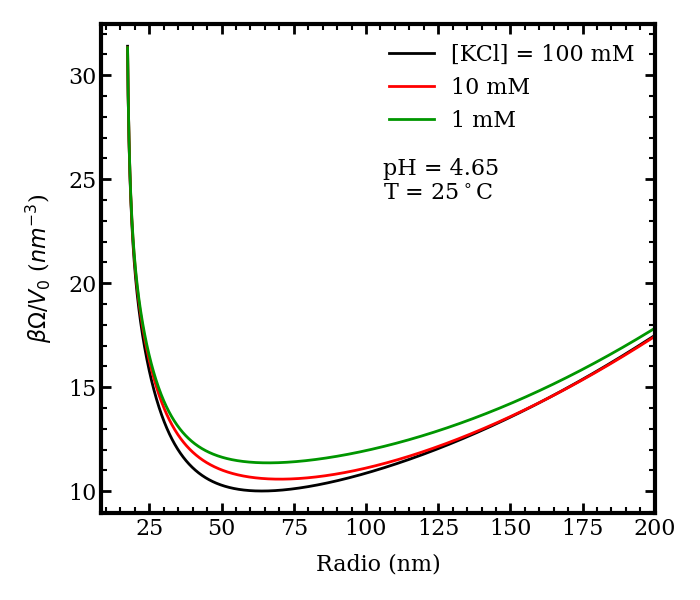
\includegraphics[width=1\linewidth]{Figures/graph-mc/interna.png}
	\caption{Energ\'ia interna para los cambios de tamaño de un nanogel...}
	\label{fig:mc:omega}
\end{figure*}


Por otro lado la energ\'ia intermolecular, $\Delta U_{inter}$, viene dada por la interacci\'ion de a pares de todos los nanogeles en soluci\'on. 
Para esta interacci\'on de a pares se ha utilizado un potencial combinado: Hertz-Yukawa. Este potencial fue previamente utilzado en \addcite[weyer2018concentration], en los cuales \addcite[weyer2018concentration] 
estudiaron la hinchaz\'on y las propiedades estructurales de suspensiones de microgeles i\'onicos su teor\'ia inlcuye las interacciones el\'asticas efectivas de Hertz y una teor\'ia de interacciones electrost\'aticas efectivas dependientes de la densidad (Yukawa). 
(un poco m\'as de los potenciales)
\textcolor{red}{Porque los podemos usar para nuestro sistema..}
Estamos trabajamos con materiales blandos que son deformables, por tando es posible modelarlos usando un potencial de Hertz, en el cual se considera la superposici\'on de las part\'iculas involucradas.
Yukawa por su parte es un potencial del tipo columbico mediado por el medio dilectrico en el que se encuentra. Se ven involucradas las cargas que envuelven a cada nanogel considerando la longitud de Debye. 
Podemos resumir nuestro potencial total de trabajo como:

\begin{align}
	U_{inter}(r) = \begin{cases} U_H + U_Y & \text{if } r \leq a_i + a_j \\ U_Y & \text{if } r > a_i + a_j \end{cases} 
	\label{eq:HY-potential}
\end{align}

en donde $r$ es la distancia entre dos nanogeles, definida como la distancia de sus centros. 
$a_i$ y $a_j$ representan los radios de el nanogel $i$ y $j$ respectivamente. Por ello la condici\'on $r \leq a_i +a_j$ representa la superposici\'on de estas particulas, deformandose y entrando en juego el potencial de Hertz.
Para mayores distancia a la suma de los radios de cada nanogel se pone en juego el potencial de Yukawa. Para el cual se define:
\begin{align}
	\beta u_Y(r) = q_i q_j \frac{e^{\kappa(a_i + a_j)}}{(1 +\kappa a_i)(1 + \kappa a_j)} \frac{e^{-\kappa r}}{r} 
	\label{eq:yukawa}
\end{align}

En donde $q_i$ y $q_j$ son las cargas netas que poseen los nanogeles $i$ y $j$ respectivamente. El valor $\kappa$ corresponde a la constante de apantallamiento de Debye. 
El pontecial de Hertz, $U_H$, se define como:
 

\begin{align}
	\begin{aligned}
		& \beta u_H (r) = \left(\frac{1-r}{a_i + a_j}\right)^{5/2}\times b_{12} \\
	\end{aligned}
\end{align}


En donde $b_{12}$ es la constante de interacci\'on entre las part\'iculas la cual depende de las propiedades el\'asticas del nanogel a trav\'es del m\'odulo de Young $\Lambda$ y el radio de Poisson $\nu$. \addcite[landau] La teor\'ia de escalado en sistemas de redes polim\'ericas predice que en buenos solventes \addcite que el m\'odulo de Young  escala linealmente con la temperatura y la densidad de los entrecruzamientos (o n\'umero de cadenas): $\Lambda \approx TN_{ch}/v$. Cuanto m\'as densos sean los entrecruzamientos, m\'as r\'igido ser\'a el gel.
Con lo cual podemos definir $b_{12}^\ast = \beta b_{12}$ el cual nos independiza de la temperatura y solo tenemos la dependencia con el n\'umero de cadenas ($N_{ch}$) y grado de entrecruzamiento de nuestro nanogel. 


\subsection{Potencial zeta ($\zeta$)}


Adem\'as de poder observar las fluctuasiones en los cambio de tamaño de los nanogeles es posible el calculo de ciertas propiedades de las mismas. Entre ellas estan el potencial zeta ($\zeta$).
Este potencial se define como...
El potencial zeta es una medida de la carga el\'ectrica neta en la superficie de una part\'icula coloidal, en este caso un nanogel. El potencial zeta afecta la estabilidad de las part\'iculas coloidales, su viscosidad y su interacci\'on con otras part\'iculas.
En los nanogeles, el potencial zeta se genera por las cargas el\'ectricas de las cadenas polim\'ericas que forman la red del gel. Las cadenas  pueden tener carga positiva o negativa, dependiendo de los grupos funcionales que contengan. De este modo el potencial zeta puede ser positivo, negativo o neutro.

El potencial zeta de un nanogel afecta su estabilidad de varias maneras. Cuando el potencial zeta es positivo, los nanogel se repelen entre s\'i, lo que hace m\'as estable en soluci\'o. Cuando el potencial zeta es negativo, las part\'iculas del nanogel se atraen entre s\'i, lo que puede hacer que los nanogeles se aglomeren.
Las cargas negativas de las superficies de los nanogeles no est\'an directamente en contacto entre s\'i. Estas cargan se ecuentran  separadas por una capa de agua. El agua tiene una carga positiva neta, por lo que las cargas negativas de los nanogeles son atra\'idas por la capa de agua. Esta atracci\'on es m\'as fuerte que la repulsi\'on entre las cargas negativas, por lo que los nanogeles se aglomeran.

Luego el potencial zeta puede definirse como: \addcite[libro S\&C]

\begin{align}
	\zeta (a) \propto \frac{Z_{net}}{a} \frac{1}{1 +ka}
	\label{eq:mc:potzeta}
\end{align}


\noindent en donde  $k$ es la inversa de la lingitud de Debye, $a$ es el radio del nanogel y $Z_{net}$ es la carga neta que se observa del nanogel al considerarlo como un nano-ion \addcite[Denton 2003]. Esta carga se deriva de la interacci\'on electrost\'atica que ocurre con la part\'icula y los contraiones que lo rodean:
\begin{align}
	Z_{net}(a) = (1 + ka)e^{-ka} \frac{3Z}{k^2a^2}\left(\cosh(ka) - \frac{\sinh(ka)}{ka}\right)
	\label{eq:mc:znet}
\end{align}

\noindent en donde $Z$ es definida como la carga orginada por el grado de carga de los segmentos cargados que componen al nanogel.

\section{Fluctuaci\'on en Volumen} \label{sec:mc:fluctuacion}
Se define la fluctuaci\'on en volumen como:
\begin{align}
	\frac{\Delta V}{V} = \sqrt{\frac{k_BT}{V}\kappa_T}
\end{align}

\noindent en donde $\kappa_T$ es la incompresiblidad isot\'ermica, la cual se obtiene:

\begin{align}
	\begin{aligned}
		\kappa & = -\frac{1}{V} \left( \frac{\partial V}{\partial P}\right)_T \\
		& =\frac{1}{V} \left( \frac{\partial^2 \Omega}{\partial V^2}\right)^{-1}_T \\
		& = 12 \pi R_{eq} \left( \frac{\partial^2 \Omega}{\partial R^2}\right)^{-1}_{T,R=R_{eq}}
	\end{aligned}
\end{align}


\section{Resultados}


\begin{figure*}[!tb]
	\centering
	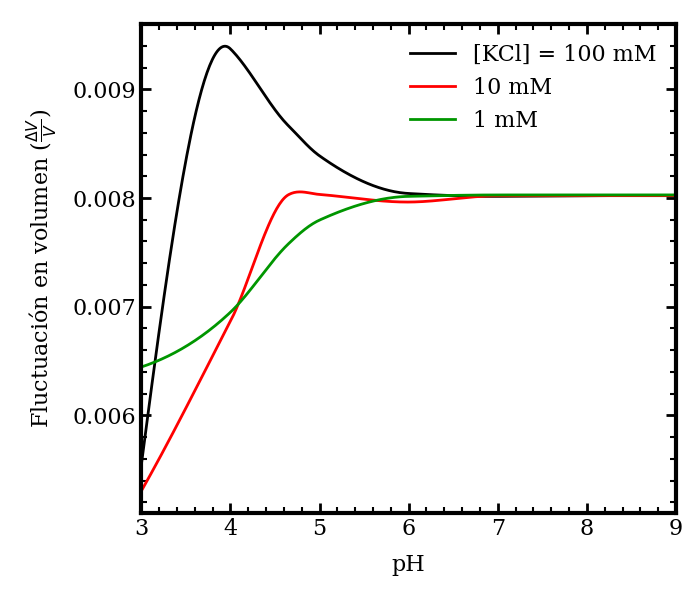
\includegraphics[width=1\linewidth]{Figures/graph-mc/dvv.png}
	\caption{Gr\'afico de la fluctuaci\'on en volumen de un nanogel aislado. El nanogel esta compuesto por $2\times 10^5$ segmentos (mon\'omeros) repartidos en 200 cadenas de 1000 cadenas cada una.}
	\label{fig:mc:dvvi}
\end{figure*}
En la figura \ref{fig:mc:dvvi} se observa la fluctuaci\'on en tama\~no de un nanogel aislado, la energ\'ia libre de estos sistemas es calcula usando el modelo del cap\'itulo \ref{Chapter-geles}....
La temperatura es de $25 ^\circ C$ condiciones en las cuales el NIPAM es hidrofilico y por ello las fluctuaciones mostradas en esta figura no se ven afectadas por la presencia de este co-mon\'omero.

C\'omo se puede observar la fluctuaci\'on del sistema diferentes condiciones de pH y concentraci\'on salina son despreciables. el c\'alculo de las mismas se realizaron con  lo expresado en la secci\'on \ref{sec:mc:fluctuacion}.
Dentro de estos valores de fluctuaci\'on se puede observar un aumento de la misma al aumentar el pH hasta estabilizar en valores de pH alrededor de 6.
A bajos valores de pH el nanogel no posee carga, los mon\'omeros de MAA que los componen se ecuentran desprotonados (estamos por debajo del pKa intr\'inseco del MAA) en estas condiciones un cambio en el tama\~no del nanogel con lleva la absorci\'on o liberaci\'on de solvente y de los iones presentes en el, adem\'as de la energ\'ia el\'astica que conlleva el cambio de radio.
La entrada o salida de iones conlleva un cambio en la cantidad de carga dentro del nanogel con lo cual se esperar\'ia un aumento en el grado de carga de los mon\'omeros, en estas condiciones de pH es muy desfavorable la desprotonaci\'on de la red polim\'erica. En consecuencia las fluctuaciones son las m\'as bajas de todo el rango de pHs.
En part\'icular altas concentraciones salinas promueven una desprotonaci\'on de los segmentos de MAA para peque\~nos aumentos de pH, ver figura \ref{fig:gel:f-cs}B, con lo cual la entrada de iones favorece la fluctuaci\'on en volumen del nanogel. 
Por otro lado a condiciones de pH altos, el gel se encuentra con un alto grado de carga. La salida o entrada de iones, y  con lo cual podr\'ia surgir un cambio en la carga del nanogel,  es m\'as favorable que a bajos pH y por ello se observa una fluctuaci\'on mayor. En estos valores altos de pH no hay diferencia alguna con la concentraci\'on salina. El nanogel posee tanta carga que los cambios en la salinidad no afectan a las flutuaciones.





\begin{figure*}[!tb]
	\centering
	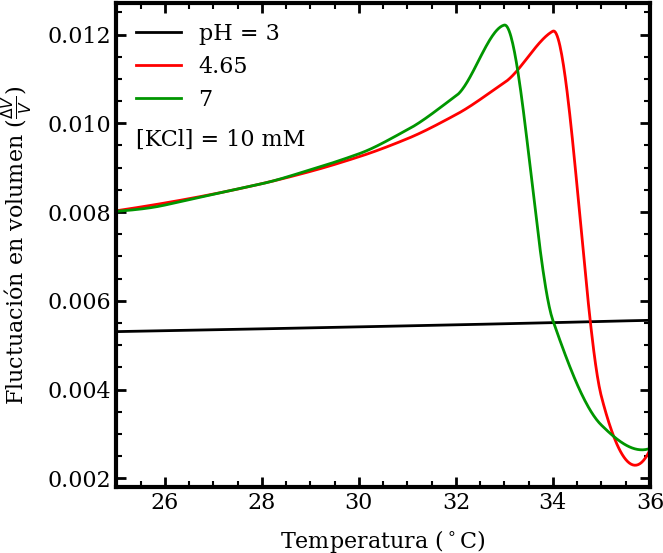
\includegraphics[width=1\linewidth]{Figures/graph-mc/fluct-T.png}
	\caption{Gr\'afico de la fluctuaci\'on en volumen de un nanogel aislado. El nanogel esta compuesto por $2\times 10^5$ segmentos (mon\'omeros) repartidos en 200 cadenas de 1000 cadenas cada una.}
	\label{fig:mc:dvv-Ti}
\end{figure*}

En la figura \ref{fig:mc:dvv-Ti} mostramos la fluctuaci\'on en volumen originada al cambiar la temperatura del sistema. Para esta figura revisaremos como se ven afectados los cambios en el tama\~no del nanogel debido al colapso de la red polim\'erica por la hidrofibicidad surgida al aumentar la temperatura. Adem\'as se presentan tres curvas mostrando los tres pH caracter\'isticos del sistema. Por abajo y arriba del pH intr\'insico pH 3 y 7 respectivamente y uno al valor del pKa del MAA aislado.
Para el pH 3 el grado de carga del gel es pr\'acticamente nulo, ver figura \ref{fig:gel:f-cs}B, por lo cual las fluctuaciones que se observan son por efecto de la temperatura. Al aumentar la temperatura se le agrega energ\'ia al sistema. Observ\'andose as\'i una peque\~na pendiente en dicha curva.

A pH 4.65 y 7 el sistema posee carga por tanto al agregarle energ\'ia al sistema (aumento de temperatura) las fluctuaciones aumentan. Esto ocurre hasta llegar a la temperatura caracter\'istica de transici\'on volum\'etrica del NIPAm, figura \ref{fig:gel:R-T}, por arriba de los $32 ^\circ$C. Despu\'es de este punto hay un colapso en la estructura del nanogel con lo cual es poco probable que se de un cambio de su tama\~no en un punto en part\'icular. ase observa un decaimiento de las fluctuaciones. 

\begin{figure*}[!tb]
	\centering
	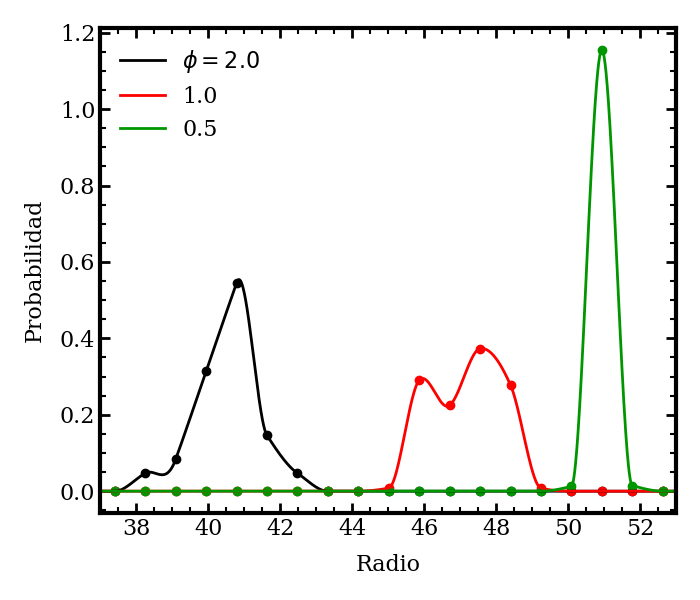
\includegraphics[width=1\linewidth]{Figures/graph-mc/denton.png}
	\caption{Gr\'afico del probabilidad de tama\~no de la soluci\'on de  nanogeles en funci\'on de la densidad... fracci\'on de volumen ocupada. nanogel m\'as flexible... 200 monomeros por cadena. 2e5 monomeros totales. radio medio aisladop = 51 nm }
	\label{fig:mc:dentos-sizes}
\end{figure*}

%\include{capitulo3}
%\include{conclu}


%% Cap'itulos incluidos despues del comando \appendix aparecen como ap'endices
%% de la tesis.


\appendix
 \appendix{B:}
 
\section{Entrop\'ia de mezcla}
Consideremos un sistema en la cual solo hay traslaciones.
En un sistema gran can\'onico la funci\'on de partici\'on viene dada por \textcolor{red}{(agregar cita libro Hill)}:
\begin{align}
	Q=\frac{q^N}{N !} && \text{, donde $q=\frac{Vz_n}{\Lambda^3}$} 
\end{align}
En donde $z_n$ corresponde al par\'ametro de  interacci\'on entre las distintas mol\'eculas. $\Lambda$ es $\frac{h}{(2\pi mkT)^{1/2}}$ .... y  $N!$  es un factor de correcci\'on para no repetir interacciones.

La energ\'ia asociada a la mezcla (entrop\'ia en fin...?) se expresa de la siguiente forma:

\begin{align}
	\begin{aligned}
		\beta F_{mix}=&-\ln Q =-\ln\frac{1}{N!}\left(\frac{VZ_n}{\Lambda^3}\right)^N \\
		&= N\ln N -N -N\ln\left(\frac{VZ_n}{\Lambda^3}\right) \\
		&=N\left[\ln\frac{N\Lambda^3}{VZ_n} -1\right]= N\left[\ln\frac{N\Lambda^3v_w}{VZ_nv_w} -1\right] \\
		&=N\left[\ln\rho v_w + \ln\frac{\Lambda^3}{Z_nv_w} -1\right] \\
		&=N\left[\ln\rho v_w + \ln\mu^0 -1\right], & \mu^0=\frac{\Lambda^3}{Z_nv_w}
	\end{aligned}
\end{align}
Es posible definir $f_{mix}=F_{mix}$ obteniendo: 
\begin{align}
	\beta f_{mix}=\rho(r)\left[\ln\rho(r) v_w + \ln\mu^0 -1\right] 
\end{align}
La expresi\'on anterior es v\'alida para un diferencial de volumen, es decir, que para obtener la energ\'ia total obtenemos:

\begin{align}
	\beta F_{mix}=\int_V{d^3r\beta f_{mix}}=\int_V{d^3r\rho(r)\left[\ln\rho(r) v_w + \ln\mu^0 -1\right]} 
\end{align}


\section{Energ\'ia qu\'imica y de mezcla del gel}

El segundo t\'ermino de la ecuaci\'on \textcolor{red}{energia} consiste en la energ\'ia qu\'imca debido a la protonaci\'on de los segmentos \'acidos del gel; adem\'as se considera la entrop\'ia de mezcla de las cadenas del mismo.

Separandolos se obtiene:

\begin{align}    
	\int_S drG(r)\frac{\left<\phi_{MAA}(r)\right>}{v_{MAA}}\left[ f(r)\beta\mu^0_{MAA^-} -(1-f(r))\beta\mu^0_{MAAH} \right]
	\label{eq-B:qca}
\end{align}

\begin{align}
	\int_S drG(r)\frac{\left<\phi_{MAA}(r)\right>}{v_{MAA}} \left[f(r)(\ln f(r)+(1-f(r))(\ln(1-f(r))\right] 
	\label{eq-B:traslacion}
\end{align}    

En donde en la \ref{eq-B:qca} $\int_S drG(r)\frac{\left<\phi_{MAA}(r)\right>}{v_{MAA}}$ multiplicado por $f(r)$ o $1-f(r)$ corresponden a $N_{MAA^-}$ y $N_{MAAH}$ respectivamente.
Falta hablar sobre el cambio de ensamble...es decir: $F= W -N\mu$.
Luego se tiene el la energ\'ia dada por potencial electrost\'atico... y finalmente los constraints... o restricciones a cumplirse por el sistema...   
\chapter{Generaci\'on de configuraciones}\label{anexo-configuraciones}



\section{Configuraciones de la red polim\'erica de un nanogel}

La red de pol\'imeros entrecruzados que forma el nanogel estudiado en el cap\'itulo \ref{Chapter-esfericas} tiene una topolog\'ia similar a la del diamante, donde los puntos de entrecruzamientos se colocan en la posici\'on original de los \'atomos de carbono y se conectan a cuatro cadenas de pol\'imeros.

Para construir esta red, primero definimos una estructura tridimensional donde todas las cadenas de pol\'imeros se alargan. Luego, solo conservamos aquellos segmentos contenidos dentro de una esfera de radio $R_{cut}$ colocada en el centro de masa de la estructura. $R_{cut}$ se elige de manera que la red resultante tenga aproximadamente $10^4$ segmentos. En total, la red que resulta de esta estrategia tiene 10026 segmentos.

\begin{figure}[!ht]
	\centering
	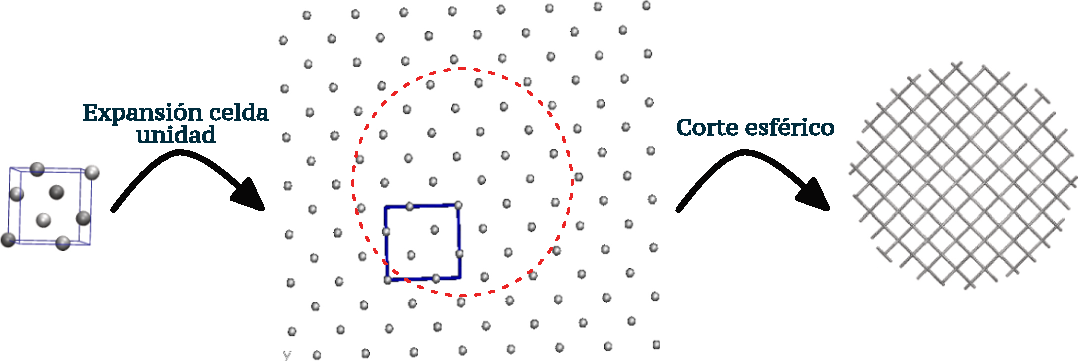
\includegraphics[width=0.90\linewidth]{Figures/graph-anexos/esquema.pdf}
	\caption{Estrucutra base para la generaci\'on de configuraciones de nanogeles}
	\label{fig:anexo:equema-gel}
\end{figure}




Originalmente, todas las cadenas de pol\'imeros conectan dos segmentos entrecruzamientes, pero como resultado del procedimiento mencionado anteriormente, algunas cadenas quedan pendientes en la superficie de la red y se conectan solo a un entrecruzamiente. Estas cadenas colgantes contienen el 22\% del n\'umero total de segmentos.

Para obtener configuraciones de esta estructura, hemos realizado simulaciones de Din\'amica Molecular utilizando GROMACS 5.1.2 \cite{lindahl2001gromacs}.
Para describir las interacciones no enlazantes entre los segmentos de la red, utilizamos un potencial de Leonard-Jones puramente repulsivo con un desplazamiento.

\begin{equation}
	V_{LJ}(r_{ij})=\begin{cases}
		4\epsilon \left[\left(\frac{\sigma}{r_{ij}}\right)^{12} - \left(\frac{\sigma}{r_{ij}}\right)^{6}\right] + \epsilon & \text{si $r_{ij} < 2^{1/6}\sigma$}\\
		0 & \text{de otro modo}.
	\end{cases}
\end{equation}



Donde $\epsilon = 1 k_BT$ y $\sigma = $ 0.5 nm, y $r_{ij}$ es la distancia entre los segmentos $i$ y $j$.
Para generar una variedad de configuraciones compactas de la estructura polim\'erica, en algunas simulaciones tambi\'en aplicamos una restricci\'on de posici\'on radial.
Este potencial se utiliza para restringir part\'iculas (en nuestro caso, los segmentos entrecruzadores de la red) a una regi\'on esf\'erica espec\'ifica del volumen de simulaci\'on.
Esta regi\'on esf\'erica esta delimitada por un radio $r_{fb}$.
De manera simplificada, la energ\'ia potencial asociada con esta fuerza externa tiene la siguiente forma:

\begin{equation}
	V_{fb}(r_i)=\begin{cases}
		0 & \text{si $r_{i} < r_{fb}$}\\
		\frac{1}{2}k_{fb}\left(r_i -r_{fb}\right)^2 & \text{de otro modo}.
	\end{cases}
\end{equation}


Donde $r_i$ es la distancia entre la posici\'on del segmento entrecruzante $i$ y el centro de masa de la red, y $k_{fb}$ es la constante de fuerza.

Un enfoque similar puede utilizarse para generar conformaciones de red elongadas (hinchadas). En este caso, aplicamos un potencial arm\'onico que restringe las part\'iculas fuera de una regi\'on esf\'erica espec\'ifica. Esta situaci\'on se describe utilizando valores negativos de $r_{fb}$, y este potencial solo se aplica a los entrecruzamientos m\'as superficiales de la red. M\'as detalles sobre estos potenciales con fondo plano se pueden encontrar en la referencia \cite{GROMACSRestraints}.

Para generar conformaciones compactas, hemos realizado simulaciones de Din\'amica Molecular utilizando $r_{fb} =$ 17.5, 20, 22.5 y 25$\sigma$.

Para conformaciones hinchadas, hemos utilizado valores de $r_{fb}$ desde $-80\sigma$ hasta $-50\sigma$ con un paso de $5\sigma$; y luego desde $-50\sigma$ hasta -27.5$\sigma$ con un paso de 2.5$\sigma$. Estos valores se referencian a la red libre (sin la restricci\'on potencial) que tiene un radio aproximado de $26\sigma$.
Se ha utilizado $k_{fb} = 50\frac{\varepsilon}{\sigma^2} $.



\begin{figure}[!ht]
	\centering
	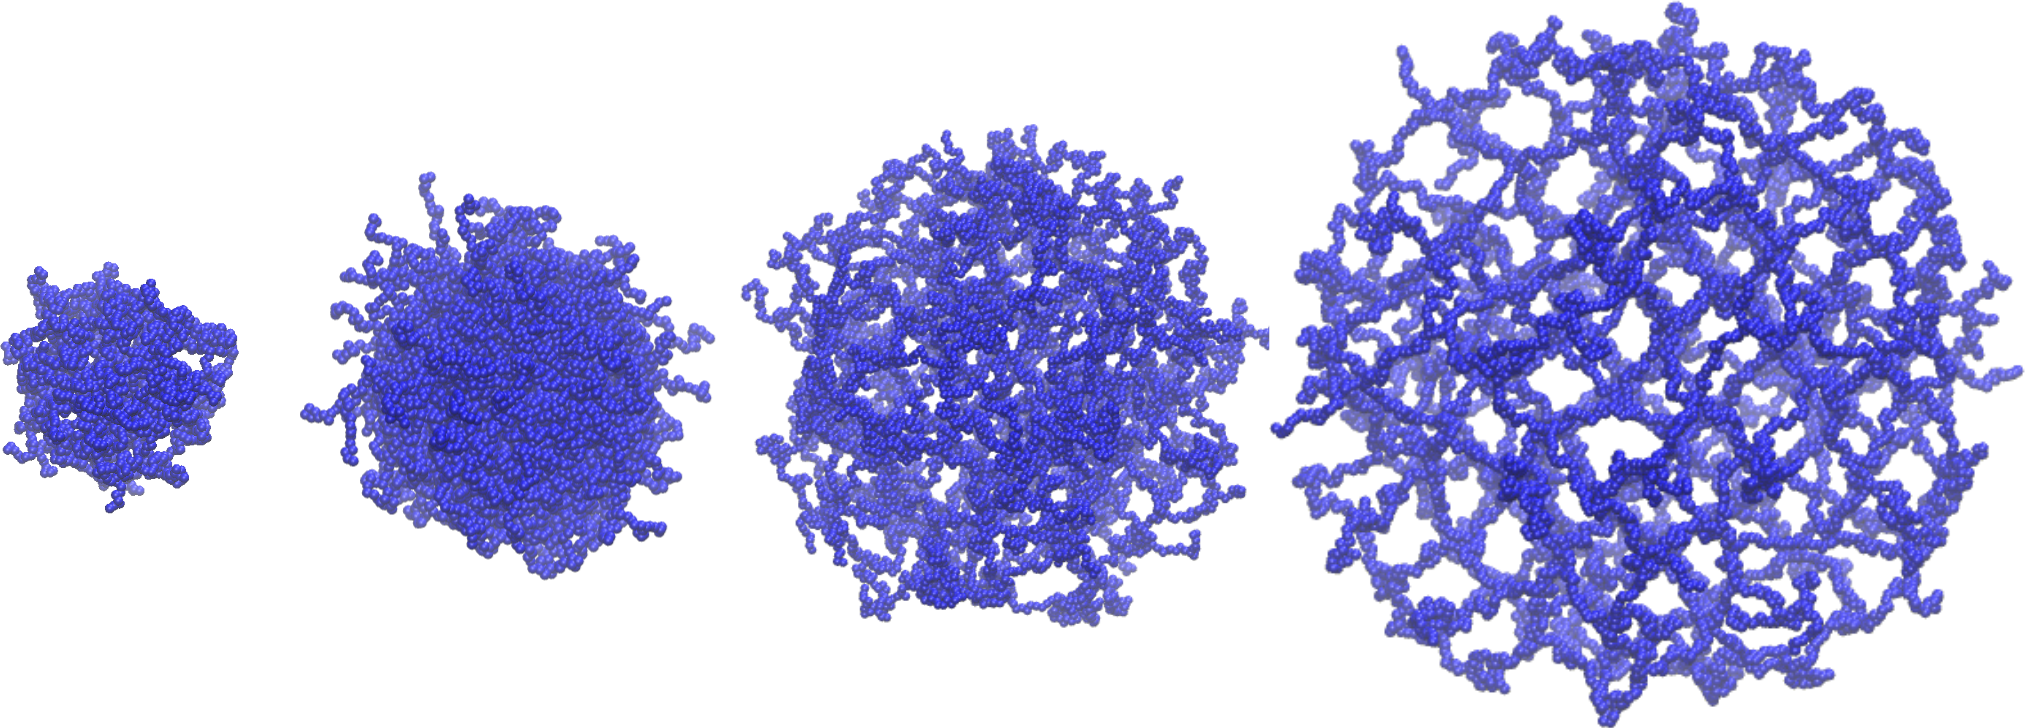
\includegraphics[width=0.5\linewidth]{Figures/graph-anexos/geles_radios.png}
	\caption{Diferentes configuraciones (a escala) con simulaciones donde se aplican diversos potenciales arm\'onicos de restricci\'on.}
	\label{fig:anexo:geles}
\end{figure}



En cada simulaci\'on de DM, el sistema se equilibr\'o durante 5 ns y luego la simulaci\'on continu\'o durante otros 10 ns. Durante este tiempo de producci\'on, se registr\'o una configuraci\'on cada 20 ps, lo que resulta en un total de 500 configuraciones por simulaci\'on y un total de 10000 configuraciones para la estructura del nanogel



%\newpage
%\thispagestyle{empty}
%\null
\chapter{Resoluci\'on num\'erica: Teor\'ia Molecular}\label{sec:film:reso-numerica}


\section{Films polim\'ericos}

La obtenci\'on de resultados a partir de la teor\'ia planteada en los cap\'itulos \ref{Chapter-film} y \ref{Chapter-esfericas} requiere la soluci\'on num\'erica de ecuaciones integro-diferenciales. Para tal prop\'osito es conveniente pasar de un sistema continuo a uno discreto. 
La discretizaci\'on de nuestro modelo se realiza en capas de espesor $\delta$. 
En particular, para el cap\'itulo \ref{Chapter-film}, la suma sobre cada uno de estas capas reemplazan a las integrales a lo largo del eje $z$, esto se debe a la simetr\'ia sobre los ejes $x$ e $y$ que se ha utilizado para el desarrollo de la TM para hidrogeles de films polim\'ericos.

Por ejemplificar este cambio, la ecuaci\'on de incompresibilidad expresada en ec. \ref{eq:film:constraint} es reescrita como:


\begin{align}
	\begin{aligned}
		1=  {\left[\sum_{\gamma}\rho_\gamma(i_z) v_\gamma + \sum_\lambda{\left<\rho_{ads,\lambda}(i_z)\right>v_\lambda} + \left<\rho_{MAA}(i_z)\right>v_{MAA} \right]},~ con \quad  i_z =1,2,3.., n_z
	\end{aligned}
	\label{eq:film:discreto-constraint}
\end{align}

Esta expresi\'on nos permite resolverla en cada una de las capas $i_z$, cuya posici\'on es descrita usando la coordenada $z_i = (i_z -0.5)\delta$, lo cual las ubica en el centro de cada capa. $i_z$ toma los valores de 1 a $n_z$, donde se toma a $n_z$ lo suficientemente grande para que las densidades de cada una de las especies involucradas, as\'i como tambi\'en el potencial electrost\'atico, converjan a sus valores en el ba\~no de la soluci\'on (el bulk de la soluci\'on).
Es decir: $\rho_\gamma(n_z) = \rho^b_\gamma$, $\rho_{ads}(\theta,n_z) = \rho^b_{ads}(\theta)$ y $\psi(n_z) = \psi^b =0$.
Para valores de $n_z \geq 500$ es posible obtener estas condiciones (dado que no son impuestas per se en la teor\'ia).

Reescribiendo las expresiones de los funcionales de la secci\'on \ref{sec:film-teoria}, obtenemos para la densidad discreta de las especies libres:

\begin{align}
	\rho_\gamma(i_z)v_w = a_\gamma \exp\left[-\beta q_\gamma\psi(i_z)\right] \exp\left[-\beta v_\gamma\pi(i_z)\right]
\end{align}


El grado de disociaci\'on para los segmentos de MAA que componen la red polim\'erica de nuestro film, de la ecuaci\'on \ref{eq:film:degree-film}:

\begin{align}
	\frac{f(i_z)}{1-f(i_z)} = \left(\frac{a_{H^+}}{K^0_{a,MAA}}\right)^{\mp 1} \exp[-\beta q_{MAA} \psi(i_z)]
\end{align}

An\'alogamente para el adsorbato, ecuaci\'on \ref{eq:film:degree-protein}:

\begin{align}
	\frac{f_\tau(i_z)}{1-f_\tau(i_z)} = \left(\frac{a_{H^+}}{K^0_{a,\tau}}\right)^{\mp 1} \exp[-\beta q_\tau \psi(i_z)]
\end{align}

\noindent en donde $\tau$ hace referencia a los segmentos del adsorbato. Y en la que se tiene en cuenta que el exponente $-1$, para segmentos \'acidos y  $+1$ para los b\'asicos.

La densidad de los segmentos que compone la red polim\'erica se expresa como:
\begin{align}
	\left< \rho_{MAA}(i_z)\right> = \sum_\alpha P(\alpha)\rho_{MAA}(\alpha, i_z)
\end{align}

En donde se redefine $P(\alpha)$:


\begin{align}
	\begin{aligned}
		P(\alpha) = &\frac{1}{Q}\exp\left[ -A \delta \sum^{n_z}_{i_z = 1} \rho_{MAA}(\alpha, i_z) \ln f(i_z)\right] \\
		%%%%
		&\exp\left[ -A\delta \sum^{n_z}_{i_z = 1}  \rho_{MAA}(\alpha, i_z) \beta q_{MAA} \psi(i_z)\right] \\
		& \exp\left[ -A\delta \sum^{n_z}_{i_z = 1}  \rho_{MAA}(\alpha, i_z) \beta v_{MAA} \pi(i_z)\right] 
	\end{aligned}
\end{align}

\noindent en donde $\psi(i_z)$ y $\pi(i_z)$ son los valores discretos de la interacci\'on de estos potenciales. Adem\'as $\rho_{MAA}(\alpha, i_z)$ es la distribuci\'on discreta para una conformaci\'on $\alpha$ la cual son provistas por el tipo de modelo molecular a usar.

La densidad discreta del adsorbato  se expresa:


\begin{align}
	\begin{aligned}
		\rho_{ads}(\theta, i_z)v_w = &\tilde{a}_{ads} \prod_\tau\exp\left[-A \delta \sum^{n_z}_{j_z = 1} n_\tau(\theta,i_z,j_z) \ln f_\tau(j_z)\right] \\
		& \prod_\lambda \exp \left[-A \delta \sum^{n_z}_{j_z = 1}  n_\lambda(\theta,i_z, j_z)[v_\lambda\beta\pi(j_z) + q_\lambda \psi(j_z)] \right]
	\end{aligned}
\end{align}

Finalmente discretizando la ecuaci\'on de Poisson, para el pontencial electrost\'atico, obtenemos:

\begin{align}
	\epsilon \frac{\psi(i_z +1) + \Psi(i_z -1) +2\psi(i_z)}{\delta^2} = \left< \rho_q(i_z)\right>
	\label{eq:film:discreto-poisson}
\end{align}

\noindent en esta expresi\'on se ha reemplazado la derivada segunda el potencial por su diferencia finita. Adem\'as la densidad discreta de carga se define:


\begin{align}
	\left<\rho_q(i_z)\right> = \sum_{\gamma } {\rho_\gamma(i_z) q_\gamma + \sum_\tau{f_\tau(i_z) \left<\rho_{ads,\tau}(i_z)\right> q_\tau} +  f(i_z)\dfrac{\left<\phi_{MAA}(i_z)\right>}{v_{MAA}}q_{MAA}}
	\label{eq:film:rho_charge-discreto}
\end{align}


As\'i como fueron definas las condiciones de contorno en la ecuaci\'on \ref{eq:film:contorno} es necesario redefinirla para el sistema discreto. Estas condiciones deben satisfacer el desvanecimiento del potencial electrost\'atico, $\psi(n_z) =0 $. Adem\'as se debe cumplir que la derivada del mismo entre la superficie de soporte y el film se anule.
Para ello es necesario agregar una capa $i_z = 0$.
Y resultando:
\begin{align}
	\frac{\psi(1) - \psi(0)}{\delta} = 0
\end{align}

\noindent lo que implica que $\psi(0) =  \psi(1)$.

En resumen dadas las condiciones del bulk de la soluci\'on, o condiciones de laboratorio, compuestas por el pH, concentraci\'on de sal y adsorbatos, temperatura, restar\'ia conocer las cantidades $\psi(i_z)$ y $\pi(i_z)$ para cada capa $i_z$. Variables que pueden ser obtenidas al resolver en cada capa las ecuaciones \ref{eq:film:discreto-constraint} y \ref{eq:film:discreto-poisson}.
De esta forma el n\'umero de ecuaciones totales a resolver es $2n_z$ (dos por cada capa). el n\'umero de t\'erminos de cada ecuaci\'on es dependiente de la cantidad de especies involucradas con sus respectivas conformaciones. 
Este sistema de ecuaciones es resuelto usando el m\'etodo de Newton con Jacobiano libre, implementado en c\'odigos FORTRAN desarrollados en el grupo de trabajo.



\section{Nanogeles estructurados}


Para obtener resultados de la minimizaci\'on de la energ\'ia, las ecuaciones integro-diferenciales no lineales descritas en el cap\'itulo \ref{Chapter-esfericas} ( secciones \ref{sec:esf:tm} y \ref{sec:esf:bulk}) deben resolverse num\'ericamente. Para lograr esto, el volumen del sistema se divide en capas de espesor $\delta = $0.5. En esta divisi\'on se ha considerado una simetr\'ia radial 

En las ecuaciones presentadas, las sumas sobre capas reemplazan las integrales a lo largo de la coordenada $r$, mientras que las diferencias finitas reemplazan las derivadas.

Reescribiendo, la restricci\'on de incomprensibilidad se expresa como:

\begin{align}
	\begin{aligned}
		1=  {\sum_{\gamma}\rho_\gamma(i_r) v_\gamma + \sum_\lambda{\left<\rho_{pro,\lambda}(i_r)\right>v_\lambda} + \sum_i{\left<\phi_i(i_r)\right>}}
		\label{eq:esf:pi-ir}
	\end{aligned}
\end{align}

Lo que nos da una ecuaci\'on para cada capa $i_r$, en donde cada posici\'on es descrita por la coordenada $r_i = (i_r -0.5)\delta$. 
La variable $i_r$ toma valores de $1$ a $n_r$, en donde $n_r$ es un n\'umero suficientemente grande de capas para que se satisfagan las restricciones impuestas en nuestro sistema. Entre ellas
$\rho_\gamma(n_r) \approx \rho_\gamma^b$, $\rho_{pro}(\theta,n_r) \approx \rho_{pro}^b(\theta)$ y $\psi(n_r) \approx \psi^b = 0$.

Con estas consideraciones podemos reescribir:


\begin{align}
	\frac{f(j_r)}{1-f(j_r)}= \left(\frac{a_{H^+}}{k^0_{a,j}}\right)^{\mp 1} e^{-\beta q_{MAA^-}\psi(i_r)}
\end{align}


Para las especies libres, sin considerar la prote\'ina, ecuaci\'on \ref{eq:esf:rho-libres}:

\begin{align}
	\rho_\gamma(i_r)v_w = a_\gamma \exp{[-\beta \psi(i_r)q_\gamma]} \exp{[-\beta\pi(i_r) v_w]}
\end{align}

La densidad local de la prote\'ina  se escribe, ecuaci\'on \ref{eq:esf:rho-pro}:

\begin{align}
	\begin{aligned}
		\rho_{pro}(\theta, i_r)v_w = &\tilde{a}_{pro} \prod_\tau\exp\left[ \sum^{n_r}_{j_r = 1} \tilde{m}_\tau(\theta,i_r,j_r) \ln f_\tau(j_r)\right] \\
		& \hspace{1em} \times \prod_\lambda \exp \left[ \sum^{n_r}_{j_r = 1} \tilde{m}_\lambda(\theta,i_r, j_r)\left(\beta\pi(j_r) v_\lambda+ \beta \psi(j_r)q_\lambda\right) \right]
	\end{aligned}
\end{align}

La probabilidad de las configuraciones de la red polim\'erica $P(\alpha)$: 

\begin{align}
	\begin{aligned}
		P(\alpha)&= \frac{1}{Q}\prod_{r_j}\prod_i \exp\left[{- {\beta\pi(r_j) \tilde{\phi}^i_r(\alpha,r_j)}}\right] \\
		& \times \prod_{r_j} \exp \left[ - \beta \psi(r_j)\frac{\tilde{ \phi}^{MAA}_r(\alpha,r_j)}{v_{MAA}} q_{MAA}  \right] \\
		& \times \prod_{r_j} \exp\left[ - { \ln(f(r_j))\frac{\tilde{ \phi}^{MAA}_r(\alpha,r_j)}{v_{MAA}}}\right] \\
	\end{aligned}
\end{align}

\noindent donde:

\begin{align}
	\tilde{ \phi}^{MAA}_r(\alpha,r_i) = \int_{r_i -\delta/2}^{r_i + \delta/2} dr \, \phi^{MAA}_r(\alpha,r)
\end{align}

La ecuaci\'on de Poisson se escribe:

\begin{align}
	\epsilon \frac{\psi(i_r +1) -2 \psi(i_r) + \psi(i_r -1)}{\delta ^2} + 2\epsilon \frac{\psi(i_r +1) -\psi(i_r)}{(i_r -0.5)\delta ^2}= -\left<\rho_q(i_r)\right>
	\label{eq:esf:poisson-ir}
\end{align}

\noindent en donde la densidad de carga se define:

\begin{align}
	\left<\rho_q(i_r)\right> = \sum_{\gamma } {\rho_\gamma(i_r) q_\gamma + \sum_\tau{f_\tau(i_r) \left<\rho_{pro,\tau}(i_r)\right> q_\tau} +  f(i_r)\dfrac{\left<\phi_{MAA}(i_r)\right>}{v_{MAA}}q_{MAA}}
\end{align}

Nuestras condiciones de contorno se reescriben:
\begin{align}
	\frac{\psi(1) - \psi(0)}{\delta} = 0
\end{align}

Definiendo  el pH, concentraci\'on de sal y prote\'ina. temperatura, es posible calcular las variables restantes  $\pi(i_r)$ y $\psi(i_r)$ para cada capal $i_r$.
Variables que pueden ser obtenidas al resolver en cada capa las ecuaciones \ref{eq:esf:pi-ir} y \ref{eq:esf:poisson-ir} y \ref{eq:film:discreto-poisson}.
De esta forma el n\'umero de ecuaciones totales a resolver es $2n_r$ (dos por cada capa). 
Este sistema de ecuaciones es resuelto usando el m\'etodo de Newton con Jacobiano libre, implementado en c\'odigos FORTRAN desarrollados en el grupo de trabajo.

%\include{apendiceC}

%% Incluir la bibliograf'ia. Mirar el archivo "biblio.bib" para m'as detales
%% y un ejemplo.
%\bibliographystyle{unsrtnat} 
\bibliographystyle{plainnat} 
\bibliography{gel}

\end{document}
